\documentclass{article}

%**************************************************************
% Importazione package
%**************************************************************

% permette di modificare i margini
%\usepackage[top=3.1cm, bottom=3.1cm, left=2.2cm, right=2.2cm]{geometry}
\usepackage[a4paper]{geometry}

% necessario per risolvere il problema del carattere invisibile per l'a capo
% \DeclareUnicodeCharacter{00A0}{ }

% per scrivere in italiano e in inglese;
% l'ultima lingua (l'italiano) risulta predefinita
\usepackage[english, italian]{babel}

% imposta lo stile italiano per i paragrafi
\usepackage{parskip}

% fornice elenchi numerati in ordine inverso
\usepackage{etaremune}

% comandi per l'appendice
\usepackage{appendix}
\renewcommand\appendixtocname{Appendici}
\renewcommand{\appendixpagename}{Appendici}

% numera anche i paragrafi
\setcounter{secnumdepth}{6}

% elenca anche i paragrafi nell'indice
\setcounter{tocdepth}{6}

% permetti di definire dei colori
\usepackage[usenames,dvipsnames]{color}

% permette di inserire le immagini/tabelle esattamente dove viene usato il
% comando \begin{figure}[H] ... \end{figure}
% evitando che venga spostato in automatico
\usepackage{float}

% permette l'inserimento di url e di altri tipi di collegamento
\usepackage[colorlinks=true]{hyperref}

\hypersetup{
    colorlinks=true, % false: boxed links; true: colored links
    citecolor=black,
    filecolor=black,
    linkcolor=black, % color of internal links
    urlcolor=Maroon  % color of external links
}

% immagini
\usepackage{graphicx}

% permette di riferirsi all'ultima pagina con \pageref{LastPage}
\usepackage{lastpage}

% tabelle su più pagine
\usepackage{longtable}

% per avere dei comandi in più da poter usare sulle tabelle
\usepackage{booktabs}

% tabelle con il campo X per riempire lo spazio rimanente sulla riga
\usepackage{tabularx}

% multirow per tabelle
\usepackage{multirow}

% colore di sfondo per le celle
\usepackage[table]{xcolor}
%\rowcolors{2}{gray!25}{} % Colora righe alterne in grigio (non funziona bene)

% permette di fare longtable larghe tutta la pagina (parametro x)
% su Ubuntu non si può installare il pacchetto, deve essere in model/
\usepackage{tabu}

% imposta lo spazio tra le righe di una tabella
\setlength{\tabulinesep}{6pt}

% definisci un nuovo tipo di colonna P che permette di andare a capo con \newline
% e giustificata a sinistra
\usepackage{array}
\usepackage{ragged2e}
\newcolumntype{P}[1]{>{\RaggedRight \hspace{0pt}}m{#1}}

% personalizza l'intestazione e piè di pagina
\usepackage{fancyhdr}

% permette di inserire caratteri speciali
\usepackage{textcomp}

% permette di aggiustare i margini e centrare tabelle e figure
\usepackage{changepage}

%Permette di includere i grafici a barre
%IMPORTANTE: deve essere caricato prima di /pgfgantt altrimenti causa conflitto
\usepackage{pgfplots}

% permette di includere i diagrammi Gantt
% su Ubuntu non si può installare il pacchetto, deve essere in model/
\usepackage{pgfgantt}

% permette di includere i grafici a torta
\usepackage{pgf-pie}

% necessario per pgf-pie
\usepackage{tikz}

% permette i path delle immagini con gli spazi
\usepackage{grffile}

% ruota le immagini
\usepackage{rotating}

% permetti di calcolare le larghezze facendo calcoli
\usepackage{calc}


%%
%% Definizione di path globali
%%
% Path assoluta a questa directory, va passato come argomento il resto della path
\newcommand{\ModelPath}[1]{/data/sources/model/#1}

% Path per accedere a modelassets
\newcommand{\ModelAssets}[1]{\ModelPath{modelassets}/#1}

% Path globali per la ricerca di immagini
\graphicspath{
	{/data/logo/PNG}
	{/data/logo/Square}
}



\fancypagestyle{plain}{
	% cancella tutti i campi di intestazione e piè di pagina
	\fancyhf{}
	\lhead{
		
\includegraphics[width=1.5cm, keepaspectratio=true]{argo_icona.png}
		\parbox[b]{5cm}{
			\emph{\GroupName{}} \vspace{0pt} \\
			\emph{Progetto \ProjectName{}} \vspace{0pt}
		}
	}
	\chead{}


	\lfoot{
		\DocTitle{} \\
		% differenzia a seconda che \DocVersion{} stampi testo o no
		\setbox0=\hbox{\DocVersion{}\unskip}\ifdim\wd0=0pt
			% nulla
		\else
			v \DocVersion{}
		\fi
	}
	\rfoot{\thepage{} di \pageref{LastPage}}

	% Visualizza una linea orizzontale in cima e in fondo alla pagina
	\renewcommand{\headrulewidth}{0.3pt}
	\renewcommand{\footrulewidth}{0.3pt}
}
\setlength{\headheight}{30pt}
\pagestyle{plain}

% allarga l'header a tutta la pagina
%\fancyhfoffset[L]{\oddsidemargin + \hoffset + 1in}
%\fancyhfoffset[R]{\evensidemargin + \marginparwidth - \marginparsep}

% Per inserire del codice sorgente formattato
\usepackage{listings}
\definecolor{darkgray}{rgb}{.4,.4,.4}
\definecolor{purple}{rgb}{0.65, 0.12, 0.82}
\definecolor{mygreen}{rgb}{0,0.6,0}
\definecolor{mygray}{rgb}{0.5,0.5,0.5}
\definecolor{mymauve}{rgb}{0.58,0,0.82}

\lstset{
  extendedchars=true,          % lets you use non-ASCII characters
  inputencoding=utf8,   % converte i caratteri utf8 in latin1, richiede \usepackage{listingsutf8} anzichè listings
  basicstyle=\ttfamily,        % the size of the fonts that are used for the code
  breakatwhitespace=false,     % sets if automatic breaks should only happen at whitespace
  breaklines=true,             % sets automatic line breaking
  captionpos=b,                % sets the caption-position to top
  commentstyle=\color{mygreen},   % comment style
  frame=none,               % adds a frame around the code
  keepspaces=true,            % keeps spaces in text, useful for keeping indentation of code (possibly needs columns=flexible)
  keywordstyle=\color{blue}\bfseries,     % keyword style
  numbers=none,               % where to put the line-numbers; possible values are (none, left, right)
  numbersep=5pt,              % how far the line-numbers are from the code
  numberstyle=\color{mygray}, % the style that is used for the line-numbers
  rulecolor=\color{black},    % if not set, the frame-color may be changed on line-breaks within not-black text (e.g. comments (green here))
  showspaces=false,           % show spaces everywhere adding particular underscores; it overrides 'showstringspaces'
  showstringspaces=false,     % underline spaces within strings only
  showtabs=false,             % show tabs within strings adding particular underscores
  stepnumber=5,               % the step between two line-numbers. If it's 1, each line will be numbered
  stringstyle=\color{red},    % string literal style
  tabsize=4,                  % sets default tabsize
  firstnumber=1      % visualizza i numeri dalla prima linea
}

% Permetti di utilizzare il grassetto per i caratteri Typewriter (per es. il font di \code{...} e \file{...})
\usepackage[T1]{fontenc}
\usepackage{lmodern}

% Permette di resettare il contatore delle note a piè di pagina ad ogni pagina
\usepackage[perpage, bottom, stable]{footmisc}
\patchcmd{\footref}{\ref}{\ref*}{}{}

% Per poter usare il carattere ° (anche nelle formule matematiche)
\usepackage{gensymb}
\usepackage{newunicodechar}
\newunicodechar{°}{\degree}

% Per importare svg
\usepackage{svg}
%\setsvg{inkscape = inkscape -z -D}

% Per numerare le tabelle e le figure con la sezione in cui si trovano
\usepackage{amsmath}
\numberwithin{figure}{section}
\numberwithin{table}{section}

% Per aggiungere un nuovo lovello di profondita (subsubparagraph)

\makeatletter
\newcounter{subsubparagraph}[subparagraph]
\renewcommand\thesubsubparagraph{%
	\thesubparagraph.\@arabic\c@subsubparagraph}
\newcommand\subsubparagraph{%
	\@startsection{subsubparagraph}    % counter
	{6}                              % level
	{\parindent}                     % indent
	{3.25ex \@plus 1ex \@minus .2ex} % beforeskip
	{-1em}                           % afterskip
	{\normalfont\normalsize\bfseries}}
\newcommand\l@subsubparagraph{\@dottedtocline{6}{12em}{5em}}
\newcommand{\subsubparagraphmark}[1]{}
\def\endsubsubparagraph{\par
	\if@noskipsec
	\ifx\@svsechd\@undefined\else\leavevmode\fi
	\fi}
\makeatletter
\def\toclevel@subsubparagraph{6}
\makeatother
% Use \ul{arg} to undlerline text
\usepackage{soul}

% Per le pagine in orientamento orizzontale
\usepackage{pdflscape}
\usepackage{afterpage}

% Set vertical space in tables
\def\arraystretch{1.5}

% Modifica font
\usepackage{fontspec}

\setmainfont{Poppins}[
    Path=\ModelAssets{poppins/} ,
    Extension = .otf ,
    UprightFont=*-Regular ,
    BoldFont=*-Bold ,
    ItalicFont=*-Italic ,
    BoldItalicFont=*-BoldItalic
]
%%%%%%%%%%%%%%
%  COSTANTI  %
%%%%%%%%%%%%%%

% In questa prima parte vanno definite le 'costanti' utilizzate da due o più documenti.

% Serve a dare la giusta formattazione alle parole presenti nel glossario
% il nome del comando \glossary è già usato da LaTeX
% permette di distingure la prima occorrenza della parola nel documento
\usepackage{xparse}
\ExplSyntaxOn
\seq_new:N \l_hernan_seq
\NewDocumentCommand{\glossario}{m}{
    \seq_if_in:NnTF{\l_hernan_seq}{#1}{
      \textit{#1\ped{\ped{G}}}
    }{
      \seq_put_left:Nn{\l_hernan_seq}{#1}
      \textit{#1\ped{\ped{G}}}
    }
}
\ExplSyntaxOff

% Meglio non mettere gli \emph dentro le costanti, in certi casi creano problemi
\newcommand{\GroupName}{Argo}
\newcommand{\GroupEmail}{argo.unipd@gmail.com}
\newcommand{\ProjectName}{ChatSQL}
\newcommand{\ProjectVersion}{}

\newcommand{\Proponente}{Zucchetti S.p.A.}
\newcommand{\Committente}{Prof. Tullio Vardanega \\ Prof. Riccardo Cardin}
\newcommand{\CommittenteInline}{Prof. Tullio Vardanega, Prof. Riccardo Cardin}
\newcommand{\ResponsabileInCarica}{\mattia}

% La versione dei documenti deve essere definita qui in global, perchè serve anche agli altri documenti
\newcommand{\VersioneNP}{1.0.1}  % Norme di Progetto
\newcommand{\VersioneAR}{1.0.2}  % Analisi dei Requisiti
\newcommand{\VersionePQ}{1.0.3}  % Piano di Qualifica
\newcommand{\VersioneG}{1.0.1}   % Glossario
\newcommand{\VersionePP}{1.0.4}  % Piano di Progetto
\newcommand{\VersioneST}{0.0.7} % Specifica Tecnica
\newcommand{\VersioneMU}{0.0.6} % Manuale Utente

% Il verbale non ha versionamento.
% Lasciare vuoto, non mettere trattini o puntini
% Non sono permessi numeri nel nome di un comando :(
\newcommand{\VersioneVprimo}{}
\newcommand{\VersioneVsecondo}{}

% Per riferirsi ad alti documenti globalmente, se la versione nella parte soprastante è vuota il numero non compare
\newcommand{\PianoDiProgetto}{\emph{Piano di Progetto v\VersionePP{}}}
\newcommand{\NormeDiProgetto}{\emph{Norme di Progetto v\VersioneNP{}}}
\newcommand{\PianoDiQualifica}{\emph{Piano di Qualifica v\VersionePQ{}}}
\newcommand{\AnalisiDeiRequisiti}{\emph{Analisi dei Requisiti v\VersioneAR{}}}
\newcommand{\Glossario}{\emph{Glossario v\VersioneG{}}}
\newcommand{\SpecificaTecnica}{\emph{Specifica Tecnica v\VersioneST{}}}
\newcommand{\ManualeUtente}{\emph{Manuale Utente v\VersioneMU{}}}

% Per riferirsi alle revisioni usare i comandi seguenti:
\newcommand{\RTB}{Requirements and Technology Baseline}
\newcommand{\PB}{Product Baseline}
\newcommand{\CA}{Customer Acceptance}

% Comandi utili per riferirsi alle varie fasi
\newcommand{\AReq}{Analisi dei Requisiti}
\newcommand{\ARischi}{Analisi dei rischi}
\newcommand{\AD}{Analisi di Dettaglio}
\newcommand{\PA}{Progettazione Architetturale}
\newcommand{\PD}{Progettazione di Dettaglio}
\newcommand{\Cod}{Codifica}
\newcommand{\VV}{Verifica e Validazione}

%Comandi shortcut per riferirsi a documenti SENZA versione
\newcommand{\PdP}{\emph{Piano di Progetto}}
\newcommand{\PdQ}{\emph{Piano di Qualifica}}
\newcommand{\NdP}{\emph{Norme di Progetto}}
\newcommand{\AdR}{\emph{Analisi dei Requisiti}}
\newcommand{\Gls}{\emph{Glossario}}
\newcommand{\ST}{\emph{Specifica Tecnica}}
\newcommand{\MU}{\emph{Manuale Utente}}

%Comando shortcut per riferirsi al Way of Working
\newcommand{\WoW}{Way of Working}

% Comandi utili per riferirsi ai componenti del gruppo (Diari delle modifiche)
\newcommand{\tommaso}{Tommaso Stocco}
\newcommand{\sebastiano}{Sebastiano Lewental}
\newcommand{\marco}{Marco Cristo}
\newcommand{\riccardo}{Riccardo Cavalli}
\newcommand{\raul}{Raul Pianon}
\newcommand{\martina}{Martina Dall'Amico}
\newcommand{\mattia}{Mattia Zecchinato}


% Comandi utili per riferirsi ai ruoli di progetto
%% non rimuovere i caratteri % gestiscono gli spazi
\NewDocumentCommand{\Responsabile}{o}{%
  \IfNoValueTF{#1}
    {\textit{responsabile di progetto}}
    {\textit{Responsabile di progetto}}%
}
\NewDocumentCommand{\Amministratore}{o}{%
  \IfNoValueTF{#1}
    {\textit{amministratore}}
    {\textit{Amministratore}}%
}
\NewDocumentCommand{\Analista}{o}{%
  \IfNoValueTF{#1}
    {\textit{analista}}
    {\textit{Analista}}%
}
\NewDocumentCommand{\Progettista}{o}{%
  \IfNoValueTF{#1}
    {\textit{progettista}}
    {\textit{Progettista}}%
}
\NewDocumentCommand{\Programmatore}{o}{%
  \IfNoValueTF{#1}
    {\textit{programmatore}}
    {\textit{Programmatore}}%
}
\NewDocumentCommand{\Verificatore}{o}{%
  \IfNoValueTF{#1}
    {\textit{verificatore}}
    {\textit{Verificatore}}%
}
\NewDocumentCommand{\Redattore}{o}{%
  \IfNoValueTF{#1}
    {\textit{redattore}}
    {\textit{Redattore}}%
}

\NewDocumentCommand{\Amministratrice}{o}{%
  \IfNoValueTF{#1}
    {\textit{amministratrice}}
    {\textit{Amministratrice}}%
}
\NewDocumentCommand{\Programmatrice}{o}{%
  \IfNoValueTF{#1}
    {\textit{programmatrice}}
    {\textit{Programmatrice}}%
}
\NewDocumentCommand{\Redattrice}{o}{%
  \IfNoValueTF{#1}
    {\textit{redattrice}}
    {\textit{Redattrice}}%
}

% FIXME: rimuovere
% \newcommand{\Responsabile}{\textit{responsabile di progetto}}
% \newcommand{\Amministratore}{\textit{amministratore}}
% \newcommand{\Analista}{\textit{analista}}
% \newcommand{\Progettista}{\textit{progettista}}
% \newcommand{\Programmatore}{\textit{programmatore}}
% \newcommand{\Verificatore}{\textit{verificatore}}
% \newcommand{\Redattore}{\textit{redattore}}

% \newcommand{\Amministratrice}{\textit{amministratrice}}
% \newcommand{\Programmatrice}{\textit{programmatrice}}
% \newcommand{\Redattrice}{\textit{redattrice}}


\newcommand{\ScopoDelProdotto}{}

\newcommand{\ScopoDelProdottoEng}{}

\newcommand{\GlossarioIntroduzione}{
  Allo scopo di evitare incomprensioni relative al linguaggio utilizzato nella documentazione di progetto, viene fornito un \Gls, nel quale ciascun termine è corredato da una spiegazione che mira a disambiguare il suo significato. I termini tecnici, gli acronimi e i vocaboli ritenuti ambigui vengono formattati in corsivo all'interno dei rispettivi documenti e marcati con una lettera \ped{G} in pedice. Tutte le ricorrenze di un termine definito nel \Gls\ subiscono la formattazione sopracitata.
}

%Comando per i verbali esterni (solamente quando ci sono tanti termini tecnici o ambigui)
\newcommand{\GlossarioIntroduzioneVE}{
  Allo scopo di evitare incomprensioni relative al linguaggio utilizzato nella documentazione di progetto, viene fornito un \Gls, nel quale ciascun termine è corredato da una spiegazione che mira a disambiguare il suo significato. I termini tecnici, gli acronimi e i vocaboli ritenuti ambigui vengono formattati in corsivo all'interno dei rispettivi documenti e marcati con una lettera \ped{G} in pedice. In questo documento viene formattata solamente la prima ricorrenza di un termine definito nel \Gls.
}

\newcommand{\ToBeContinued}{\textit{Continua nella prossima pagina}}

% Altri comandi utili
\newcommand{\email}{email}
\newcommand*{\sezione}[1]{\hyperref[{#1}]{sezione §\ref*{#1}}}
\newcommand*{\appendice}[1]{\hyperref[{#1}]{Appendice \autoref*{#1}}}

% Bisognerebbe aggiungere anche altri brand utilizzati spesso nei vari documenti
\newcommand{\Macos}{macOs}

%%%%%%%%%%%%%%
%  FUNZIONI  %
%%%%%%%%%%%%%%

% In questa seconda parte vanno definite le 'funzioni' utilizzate da due o più documenti.

% Comando per usare comodamente le virgolette
\newcommand{\virgolette}[1]{``#1''}

\newcommand\flextt{%
	\fontdimen2\font=0.2em% interword space
	\fontdimen3\font=0.1em% interword stretch
	\fontdimen4\font=0.1em% interword shrink
	\fontdimen7\font=0.2em% extra space
	\hyphenchar\font=`\-
}

% Serve a dare la giusta formattazione al codice inline
\newcommand{\code}[1]{\ttfamily\flextt{#1}\normalfont}

% Serve a dare la giusta formattazione a tutte le path presenti nei documenti
\newcommand{\file}[1]{\flextt{#1}}

% Permette di andare a capo all'interno di una cella in una tabella
\newcommand{\multiLineCell}[2][c]{\begin{tabular}[#1]{@{}l@{}}#2\end{tabular}}

% Per l'allineamento delle immagini
\usepackage[export]{adjustbox}

% Genera automaticamente la pagina di copertina
\newcommand{\makeFrontPage}{
  % Declare new goemetry for the title page only.
  \newgeometry{top=2cm}
  \begin{titlepage}
  \begin{center}
  \vspace*{2cm}
  \begin{center}
  
\includegraphics[width=8cm]{argo_square.png}
  \end{center}

%  \vspace{1cm}

  \begin{Huge}
  \textbf{\DocTitle{}}
  \end{Huge}

  \textbf{\emph{Gruppo \GroupName{} \, \texttwelveudash{} \, Progetto \ProjectName{}}}

  \vspace{10pt}

  \bgroup
  \def\arraystretch{1.3}
  \begin{tabular}{ r|l }
    \multicolumn{2}{c}{\textbf{Informazioni sul documento}} \\
    \hline
    \ifx\DocVersion\empty
      \ifdefined\DocData
        \ifx\DocData\empty
          % lascio vuoto
        \else
          \textbf{Data} & \DocData{} \\
        \fi
      \fi
    \else
      \textbf{Versione} & \faIcon{tag} \DocVersion{} \\
    \fi
    \textbf{Approvazione} & \multiLineCell[t]{\DocApprovazione{}} \\
    \textbf{Uso} & \DocUso{} \\
    \textbf{Distribuzione} & \multiLineCell[t]{\DocDistribuzione{}} \\
  \end{tabular}
  \egroup

  \vspace*{\fill}

  \begin{figure}[H]
	\includegraphics[height=3.5cm, center]{\ModelAssets{logo_unipd.png}}
  \end{figure}
  \end{center}
  \end{titlepage}

  % Ends the declared geometry for the titlepage
  \restoregeometry
}

%%%%%%%%%%%%%%
%  COSTANTI  %
%%%%%%%%%%%%%%

% In questa prima parte vanno definite le 'costanti' utilizzate soltanto da questo documento.
% Devono iniziare con una lettera maiuscola per distinguersi dalle funzioni.

\newcommand{\DocTitle}{Verbale Riunione 2024-05-02}
\newcommand{\DocVersion}{1.0.0}
\newcommand{\DocApprovazione}{\raul}
\newcommand{\DocUso}{Interno}
\newcommand{\DocDistribuzione}{
	\Committente{} \\
	Gruppo \GroupName{}
}

% La descrizione del documento
\newcommand{\DocDescription}{
	Durante l'incontro sono state discusse le attività svolte durante la settimana e sono stati presentati e discussi i punti per il diario di bordo del 3 maggio 2024. È stata inoltre inviata una mail alla Proponente e fissato un incontro per il 6 maggio 2024.
}

%%%%%%%%%%%%%%
%  FUNZIONI  %
%%%%%%%%%%%%%%

% In questa seconda parte vanno definite le 'funzioni' utilizzate soltanto da questo documento.

\begin{document}

\makeFrontPage

\section*{Registro delle modifiche}

\bgroup
\begin{adjustwidth}{-0.5cm}{-0.5cm}
	% MAX 12.5cm
 	\begin{longtable}{|P{1cm}|P{2.2cm}|P{2.7cm}|P{2.7cm}|>{\arraybackslash}P{3.8cm}|}
	  \hline
		\textbf{Ver.} & \textbf{Data} & \textbf{Redazione} & \textbf{Verifica} & \textbf{Descrizione} \\ 
		\hline
		\endfirsthead

		\hline
		\textbf{Ver.} & \textbf{Data} & \textbf{Redazione} & \textbf{Verifica} & \textbf{Descrizione} \\ 
		\hline
		\endhead

		\hline
		\multicolumn{5}{|r|}{{Continua nella prossima pagina}} \\ 
		\hline
		\endfoot

		\hline
		\endlastfoot

		% IN ORDINE DALLA MODIFICA PIÙ RECENTE ALLA PIÙ VECCHIA
		0.0.1 & 2024-06-09 & \martina & \riccardo & Stesura del documento \\
	\end{longtable}
\end{adjustwidth}
\egroup
\clearpage

\tableofcontents
\clearpage
\renewcommand{\listtablename}{Elenco delle tabelle}
\listoftables
\clearpage
\renewcommand{\listfigurename}{Elenco delle figure}
\listoffigures
\clearpage  

\makeatletter
\newcommand\subsubsubsection{\@startsection{paragraph}{4}{\z@}{-2.5ex\@plus -1ex \@minus -.25ex}{1.25ex \@plus .25ex}{\normalfont\normalsize\bfseries}}
\makeatother

\section{Introduzione}

\subsection{Scopo del documento}
Il presente documento si propone di offrire una trattazione esaustiva dei casi d'uso e dei \glossario{requisiti} del progetto "ChatSQL", seguendo gli \glossario{standard di qualità} dell'ingegneria del software. Tale analisi è stata condotta attraverso un'approfondita valutazione del \glossario{capitolato} C9 presentato dalla Proponente(G) Zucchetti S.p.A., integrata da una stretta collaborazione durante gli incontri dedicati.
L'obiettivo principale è definire con precisione le caratteristiche e le necessità della web application proposta, la quale verrà definita propriamente all'interno della sezione 2)[qua ci mettiamo un link].

\subsection{Scopo del prodotto}
L’utilizzo di strumenti di facilitazione basati sull’utilizzo di \glossario{Intelligenza Artificiale} si sta diffondendo in maniera esponenziale, e anche gli utenti non facenti parte dell’area IT (\glossario{Information Technology}) li utilizzano con sempre maggior frequenza per velocizzare le attività quotidiane. L’azienda Zucchetti ha proposto lo sviluppo di un’applicazione che tramite l’utilizzo di LLM (\glossario{Large Language Model}) consente la generazione di \glossario{prompt} ottimizzati all’interrogazione di modelli dati basati su \glossario{database SQL}. I \glossario{prompt} potranno essere poi proposti a servizi di LLM come ChatGPT per la generazione della \glossario{query} di interrogazione da eseguire sul database.
L'applicazione sarà implementata come una web application accessibile attraverso i principali browser come Chrome, Firefox, Edge e Safari. Gli utenti di tipo operatore potranno caricare, a seguito di autenticazione, nell’applicativo i modelli dati da poter utilizzare per la generazione dei \glossario{prompt}. Gli utenti finali potranno chiedere tramite linguaggio naturale la generazione del \glossario{prompt} basandosi su uno specifico modello di dati. Il \glossario{prompt} generato e passato ad un servizio di LLM genererà la \glossario{query} da poter eseguire.

\subsection{Glossario}
\GlossarioIntroduzione

\subsection{Riferimenti}
\subsubsection{Riferimenti normativi}
\begin{itemize}
  \item Capitolato C9 - ChatSQL:\\ \href{https://www.math.unipd.it/~tullio/IS-1/2023/Progetto/C9.pdf}{https://www.math.unipd.it/\~tullio/IS-1/2023/Progetto/C9.pdf} \\ \href{https://www.math.unipd.it/~tullio/IS-1/2023/Progetto/C9.pdf}{https://www.math.unipd.it/\~tullio/IS-1/2023/Progetto/C9p.pdf};
  \item Norme di Progetto:\\ \href{https://github.com/Argo-swe/argo-swe.github.io/blob/main/2_RTB/NormeDiProgetto.pdf}{https://github.com/Argo-swe/argo-swe.github.io/blob/main/2\_RTB/ \\ NormeDiProgetto.pdf};
  \item Verbale esterno 11-03-2024:\\ \href{https://github.com/Argo-swe/argo-swe.github.io/blob/main/1_Candidatura/Verbali/Interni/VerbaleInterno_2024-03-09.pdf}{https://github.com/Argo-swe/argo-swe.github.io/blob/main/1\_Candidatura/ \\ Verbali/Interni/VerbaleInterno\_2024-03-09.pdf};
  \item Regolamento del Progetto Didattico:\\ \href{https://www.math.unipd.it/~tullio/IS-1/2023/Dispense/PD2.pdf}{https://www.math.unipd.it/~tullio/IS-1/2023/Dispense/PD2.pdf};
  \item Linee guida per l'accessibilità (WCAG 2.1):\\ \href{https://www.w3.org/Translations/WCAG21-it}{https://www.w3.org/Translations/WCAG21-it}.
\end{itemize}

\subsubsection{Riferimenti informativi}
\begin{itemize}
  \item Dispense dal corso Ingegneria del Software: T5 - Analisi dei Requisiti:\\ \href{https://www.math.unipd.it/~tullio/IS-1/2023/Dispense/T5.pdf}{https://www.math.unipd.it/\~tullio/IS-1/2023/Dispense/T5.pdf}  \\ (Ultimo accesso: 2024-05-20);
  \item Dispense dal corso Ingegneria del Software: P2 - Diagrammi Use Case:\\ \href{https://www.math.unipd.it/~rcardin/swea/2022/Diagrammi%20Use%20Case.pdf}{https://www.math.unipd.it/\~rcardin/swea/2022/Diagrammi\_Use\_Case.pdf}  \\ (Ultimo accesso: 2024-06-21);
  \item Analisi dei requisiti e casi d'uso:\\ \href{https://www.cs.unibo.it/~cianca/wwwpages/ids/6.pdf}{https://www.cs.unibo.it/~cianca/wwwpages/ids/6.pdf}  \\ (Ultimo accesso: 2024-06-19);
  \item Strutturare i casi d'uso:\\ \href{https://guides.visual-paradigm.com/structuring-use-cases-with-base-include-and-extend-a-guide-for-effective-software-development}{https://guides.visual-paradigm.com/structuring-use-cases-with-base-include-and-extend-a-guide-for-effective-software-development}  \\ (Ultimo accesso: 2024-06-19);
  \item Casi d'uso - FAQ:\\ \href{https://analisi-disegno.com/usecases/usecases-faq}{https://analisi-disegno.com/usecases/usecases-faq/}  \\ (Ultimo accesso: 2024-06-18);
  \item Extension points:\\ \href{https://www.cs.unibo.it/gabbri/MaterialeCorsi/2.usecasediagramUML.favini.pdf}{https://www.cs.unibo.it/gabbri/MaterialeCorsi/2.usecasediagramUML.favini.pdf}  \\ (Ultimo accesso: 2024-06-19);
  \item Relazione di generalizzazione:\\ \href{https://www.geeksforgeeks.org/use-case-diagram}{https://www.geeksforgeeks.org/use-case-diagram}  \\ (Ultimo accesso: 2024-06-21);
  \item Esempi di diagrammi dei casi d'uso:\\ \href{https://www.uml-diagrams.org/use-case-diagrams-examples.html}{https://www.uml-diagrams.org/use-case-diagrams-examples.html}  \\ (Ultimo accesso: 2024-06-21).
\end{itemize}

\clearpage
\section{Requisiti di sistema}

\subsection{Requisiti software}
\par Per eseguire correttamente l'applicazione, è necessario avere \glossario{Docker} installato. I requisiti specifici dipendono dal sistema operativo in uso:
\begin{itemize}
  \item \textbf{Windows}
  \begin{enumerate}
    \item \textbf{Docker Desktop}
    \begin{itemize}
      \item Docker Desktop per Windows include Docker Engine, Docker Compose e tutte le componenti necessarie per eseguire i container;
      \item Maggiori informazioni sono disponibili qui: \href{https://docs.docker.com/desktop/install/windows-install}{https://docs.docker.com/des \- ktop/install/windows-install}.
    \end{itemize}
    \item \textbf{WSL 2 (consigliato)}
    \begin{itemize}
      \item Docker Desktop si integra con Windows Subsystem for Linux 2 (WSL 2) per eseguire container Linux in modo più efficiente;
      \item Maggiori informazioni sono disponibili qui: \href{https://docs.microsoft.com/en-us/windows/wsl/install}{https://docs.microsoft.com/en-us/windows/wsl/install}.
    \end{itemize}
  \end{enumerate}
  \item \textbf{macOS}
  \begin{enumerate}
    \item \textbf{Docker Desktop}
    \begin{itemize}
      \item Docker Desktop per macOS include Docker Engine, Docker Compose e tutte le componenti necessarie per eseguire i container;
      \item Maggiori informazioni sono disponibili qui: \href{https://docs.docker.com/desktop/install/mac-install}{https://docs.docker.com/des \- ktop/install/mac-install}.
    \end{itemize}
  \end{enumerate}
  \item \textbf{Linux}
  \begin{enumerate}
    \item \textbf{Docker Desktop}
    \begin{itemize}
      \item Docker Desktop per Linux include Docker Engine, Docker Compose e tutte le componenti necessarie per eseguire i container;
      \item Maggiori informazioni sono disponibili qui: \href{https://docs.docker.com/desktop/install/linux}{https://docs.docker.com/desktop/install/linux}.
    \end{itemize}
    \item \textbf{Docker Engine} (alternativa a Docker Desktop)
    \begin{itemize}
      \item Su Linux, è generalmente preferibile installare direttamente Docker Engine piuttosto che Docker Desktop, poiché offre un'integrazione più semplice, leggera e nativa con il sistema operativo;
      \item Maggiori informazioni sono disponibili qui: \href{https://docs.docker.com/engine/install}{https://docs.docker.com/engine/install}.
    \end{itemize}
    \item \textbf{Docker Compose} (alternativa a Docker Desktop)
    \begin{itemize}
      \item Se Docker Engine viene installato separatamente su Linux, è necessario installare anche Docker Compose per orchestrare più container;
      \item Maggiori informazioni sono disponibili qui: \href{https://docs.docker.com/compose/install}{https://docs.docker.com/compose/install}.
    \end{itemize}
  \end{enumerate}
\end{itemize}

\subsection{Requisiti hardware}
\begin{itemize}
  \item \textbf{RAM}
  \begin{itemize}
    \item \textbf{Minimo}: 4 GB;
    \item \textbf{Consigliato}: 8 GB o più (per un'esperienza ottimale).
  \end{itemize}
\end{itemize}

\subsection{Browser supportati}
\par Di seguito sono elencati i browser in cui l'applicazione è accessibile e fruibile.

\begin{table}[H]
  \centering
  \begin{tabular}{|c|c|}
      \hline
      \textbf{Browser} & \textbf{Versione} \\
      \hline
      Google Chrome & 110 e successive \\
      \hline
      Mozilla Firefox & 109 e successive \\
      \hline
      Safari & 15 e successive \\
      \hline
      Opera & 94 e successive \\
      \hline
      Microsoft Edge & 110 e successive \\
      \hline
  \end{tabular}
  \caption{Tabella dei browser supportati}
\end{table}
\clearpage
\section{Installazione}

\par Per utilizzare l'applicazione, il primo passo è copiare il codice sorgente in una cartella dedicata. Il \glossario{repository} è disponibile al seguente indirizzo:

\quad \href{https://github.com/Argo-swe/ChatSQL/tree/v2.0.1}{ChatSQL - v2.0.1} \newline

\par Per scaricare il codice sorgente vi sono due modalità principali:
\begin{enumerate}
  \item Scaricare il repository in formato zip e decomprimerlo in una cartella dedicata;
  \item Clonare il repository tramite il seguente comando:
  \begin{itemize} 
    \item \texttt{git clone https://github.com/Argo-swe/ChatSQL.git}
  \end{itemize}
\end{enumerate}

\vspace{0.5\baselineskip}
\par Una volta scaricato il codice dell'applicazione, è necessario navigare nelle cartelle \textit{backend} e \textit{frontend}, e aggiungere il file \textit{.env.local} in entrambe le cartelle. Questo file consente all'utente di impostare le variabili d'ambiente.
\section{Avvio}

\par L'applicazione può essere avviata in due modalità differenti:
\begin{enumerate}
  \item Avvio separato del front-end e del back-end:
  \begin{itemize}
    \item \texttt{docker compose up backend};
    \item \texttt{docker compose up frontend}.
  \end{itemize}
  \item Avvio combinato del front-end e del back-end:
  \begin{itemize}
    \item \texttt{docker compose up}.
  \end{itemize}
\end{enumerate}

\vspace{0.5\baselineskip}
\par Una volta avviata l'applicazione, è possibile accedervi tramite il browser all'indirizzo \texttt{http://localhost:5173}.
\clearpage
\section{Istruzioni per l'utilizzo}

\par La sezione seguente presenta le funzionalità del sistema, suddivise tra quelle destinate agli utenti e quelle riservate ai tecnici. Per ciascuna funzionalità, è inclusa un'immagine che offre un esempio visivo, con l'intento di fornire istruzioni chiare e immediate.

\par La maggior parte delle istruzioni fornite si riferisce all'utilizzo dell'applicativo con il tema chiaro e il sistema impostato in lingua italiana. Per modificare le impostazioni predefinite, consultare la \sezione{sec:tema} e la \sezione{sec:lingua} delle configurazioni generali.

\section{Impostazioni generali}

Tutte le istruzioni fornite sono riferite all'utilizzo dell'applicativo con il tema chiaro e con il sistema impostato in lingua italiana. Se si ha la necessità di cambiarlo si veda la sezione 2 e 3 delle impostazioni generali sottostanti.

Il sistema in alto a destra presenta due simboli: una rotella e un omino stilizzato. La prima è la rotella che dà accesso alle impostazioni di cui sotto e l'omino stilizzato permette l'accesso come tecnico al sistema (sezione Tecnico 6.1).

Una volta cliccata la rotella, si apre un menù a tre voci con le caratteristiche modificabili dall'utente del sistema:
\begin{enumerate}
    \item La scala di grandezza del testo
    \item La modalità di visualizzazione del sistema chiara o scura
    \item La lingua del sistema
\end{enumerate}

\subsection{Scala di grandezza del testo}

Il sistema permette di far scegliere all'utente la grandezza dei caratteri del testo tramite una scala di 5 misure diverse. Per modificare la grandezza è necessario cliccare il ``-'' o il ``+'' presenti affianco alla voce ``Scala'' che permettono rispettivamente di rimpicciolire o ingrandire il testo.

\begin{figure}[H]
    \centering
    %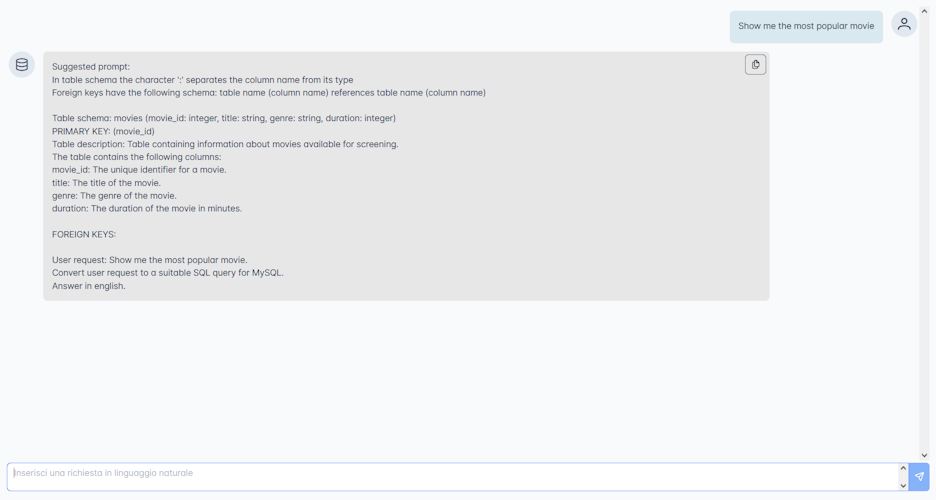
\includegraphics[width=1\textwidth]{assets/chat_example.png}
    \caption{Immagine con freccia nella scala}
  \end{figure}

\subsection{La modalità di visualizzazione del sistema chiara o scura}

Il sistema permette di impostare la modalità chiaro/scuro. Di default la modalità è chiara, ovvero il colore di sfondo del sistema è il bianco, ma è possibile cliccare nel bottoncino affianco alla voce ``Modalità scuro'' per attivare la modalità notte e avere come sfondo il colore nero.

\begin{figure}[H]
    \centering
    %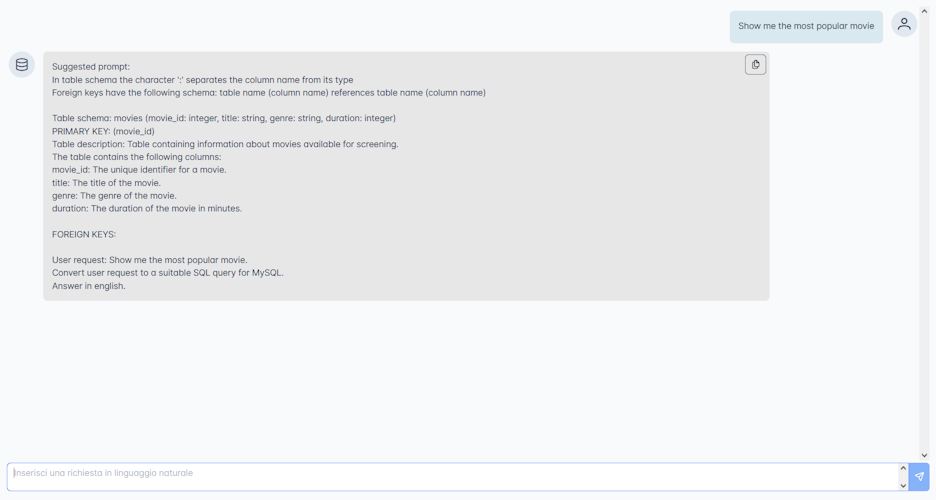
\includegraphics[width=1\textwidth]{assets/chat_example.png}
    \caption{Immagine con freccia nel modalità notte}
  \end{figure}

\subsection{La lingua del sistema}

Il sistema permette di impostare la lingua con cui il sistema si presenta, per esempio le parole dei bottoni o le voci dei menù. Questa voce non influenza la lingua con cui viene restituito il prompt dal sistema (si veda per questo la sezione 6.2.4). Le lingue possibili sono l'italiano e l'inglese.

\begin{figure}[H]
    \centering
    %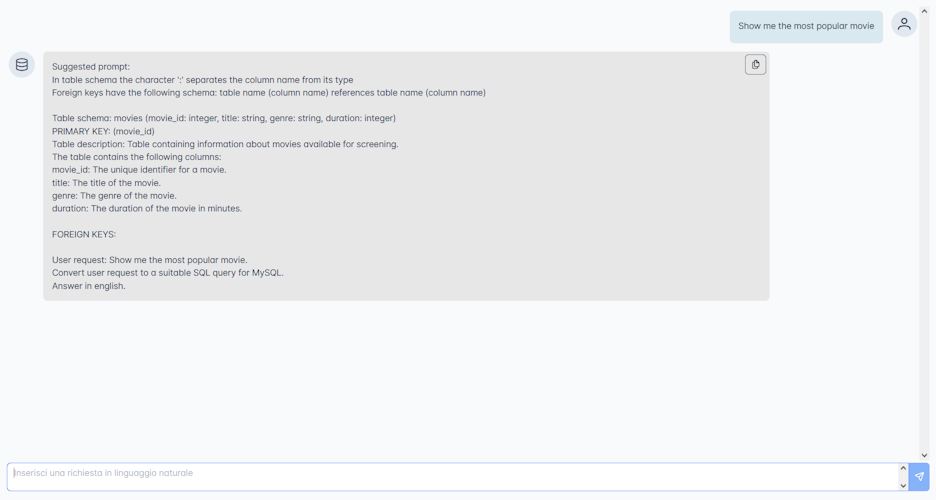
\includegraphics[width=1\textwidth]{assets/chat_example.png}
    \caption{Immagine con freccia nella lingua}
  \end{figure}

Per uscire dalle impostazioni è necessario cliccare la ``x'' in alto a destra e si tornerà al sistema con le impostazioni scelte.

\section{Sezione Utente}
\label{sec:sezUtente}

\subsection{Visualizzazione mobile}
\begin{figure}[H]
  \centering
  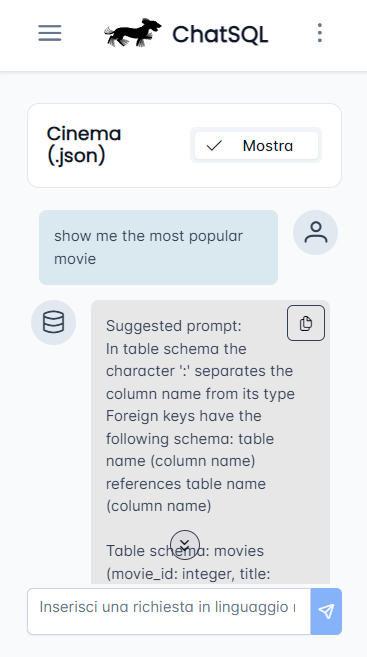
\includegraphics[width=0.50\textwidth]{assets/mobile.png}
  \caption{Versione mobile dell'applicazione}
\end{figure}
\par L'applicazione è stata progettata per essere fruibile anche da dispositivi mobili per garantire una buona esperienza d'uso con schermi touch screen di piccole dimensioni.  
\par Per migliorare la navigazione da dispositivi mobili, il menù principale, di default è nascosto e può essere aperto cliccando l'icona a tre linee 
\includegraphics[height=1.2em]{assets/dd_burger_menu.png} in alto a sinistra.
\par Le viste dell'applicazione occupano tutta la grandezza dello schermo, per dare più spazio possibile al contenuto principale.
\par Per ridurre l'ingombro dello schermo, i bottoni di login e delle impostazioni di sistema, sono accessibili mostrando un menù a tendina, cliccando sull'icona a tre puntini 
\includegraphics[height=1.2em]{assets/dd_kebab_menu.png} in alto a destra.

\subsection{Impostazioni di sistema}
Nella sezione superiore destra dell'interfaccia, cliccando sull'icona impostazioni 
\includegraphics[height=1.2em]{assets/settings_icon.png}, apparirà il menu laterale delle impostazioni di sistema.
\begin{figure}[H]
  \centering
  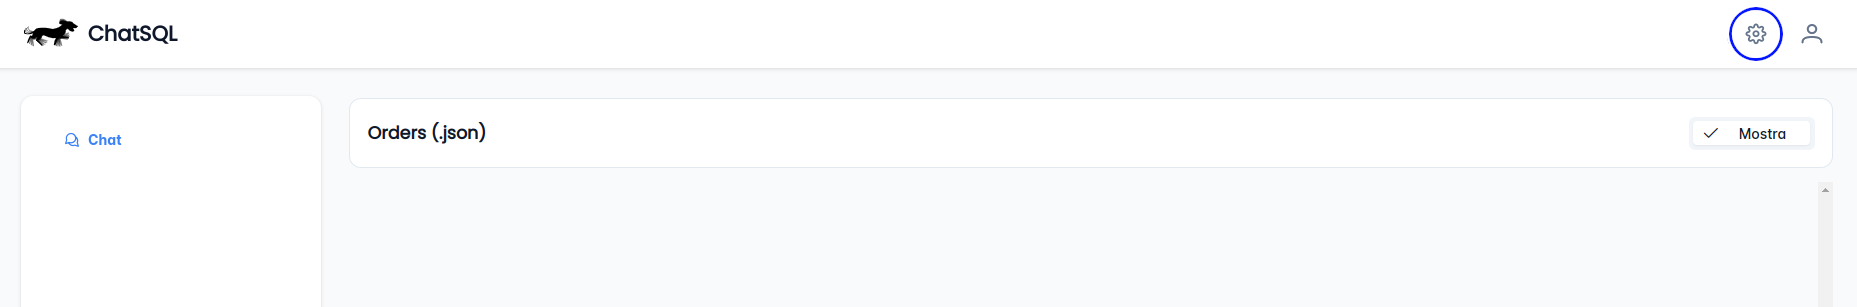
\includegraphics[width=1\textwidth]{assets/settings_topbar.png}
  \caption{Topbar con icona delle impostazioni}
\end{figure}
\begin{figure}[H]
  \centering
  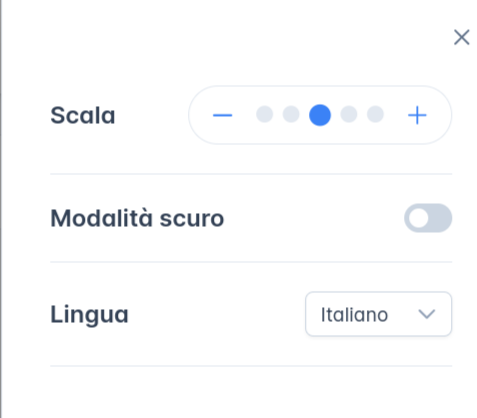
\includegraphics[width=0.50\textwidth]{assets/menu_config.png}
  \caption{Menu laterale delle impostazioni di sistema}
\end{figure}
\par Le impostazioni di sistema permettono di configurare le seguenti opzioni:
\begin{itemize}
  \item Scala: dimensioni del testo e della schermata; utile per adattare la dimensione dell'interfaccia alle proprie esigenze;
  \item Tema scuro: abilita o disabilita il tema scuro dell'interfaccia, per personalizzazione, accessibilità e comfort visivo;
  \item Lingua: selezione della lingua dell'interfaccia tra inglese e italiano (non cambia la lingua del \glossario{prompt} prodotto da ChatSQL, che rimane sempre in inglese).
\end{itemize}
\par Le modifiche apportate verranno memorizzate automaticamente, e applicate alla successiva apertura dell'applicazione.

\subsection{Workflow}
\par Nell'utilizzo di ChatSQL, il flusso più comune da seguire per ottenere una query SQL è:
\begin{enumerate}
  \item Accedere alla pagina Chat selezionandola dal menu di navigazione principale;
  \item Selezionare il \glossario{dizionario dati} desiderato;
  \item Selezionare il \glossario{DBMS desiderato};
  \item Selezionare la lingua desiderata;
  \item Inserire una richiesta in linguaggio naturale e attendere la generazione del \glossario{prompt};
  \item Copiare il prompt generato cliccando sull'apposito pulsante in alto a destra all'interno del messaggio fornito dal ChatBOT;
  \item Incollare il prompt in un modello \glossario{LLM} a scelta (come ChatGPT) e attendere la generazione della query SQL.
\end{enumerate}

\vspace{0.5\baselineskip}
\par Di seguito è riportata una figura che illustra nel dettaglio il flusso da seguire per ottenere una query SQL da utilizzare per interrogare database reali.

\begin{figure}[H]
  \fbox{
  \begin{tabular}{cc}
    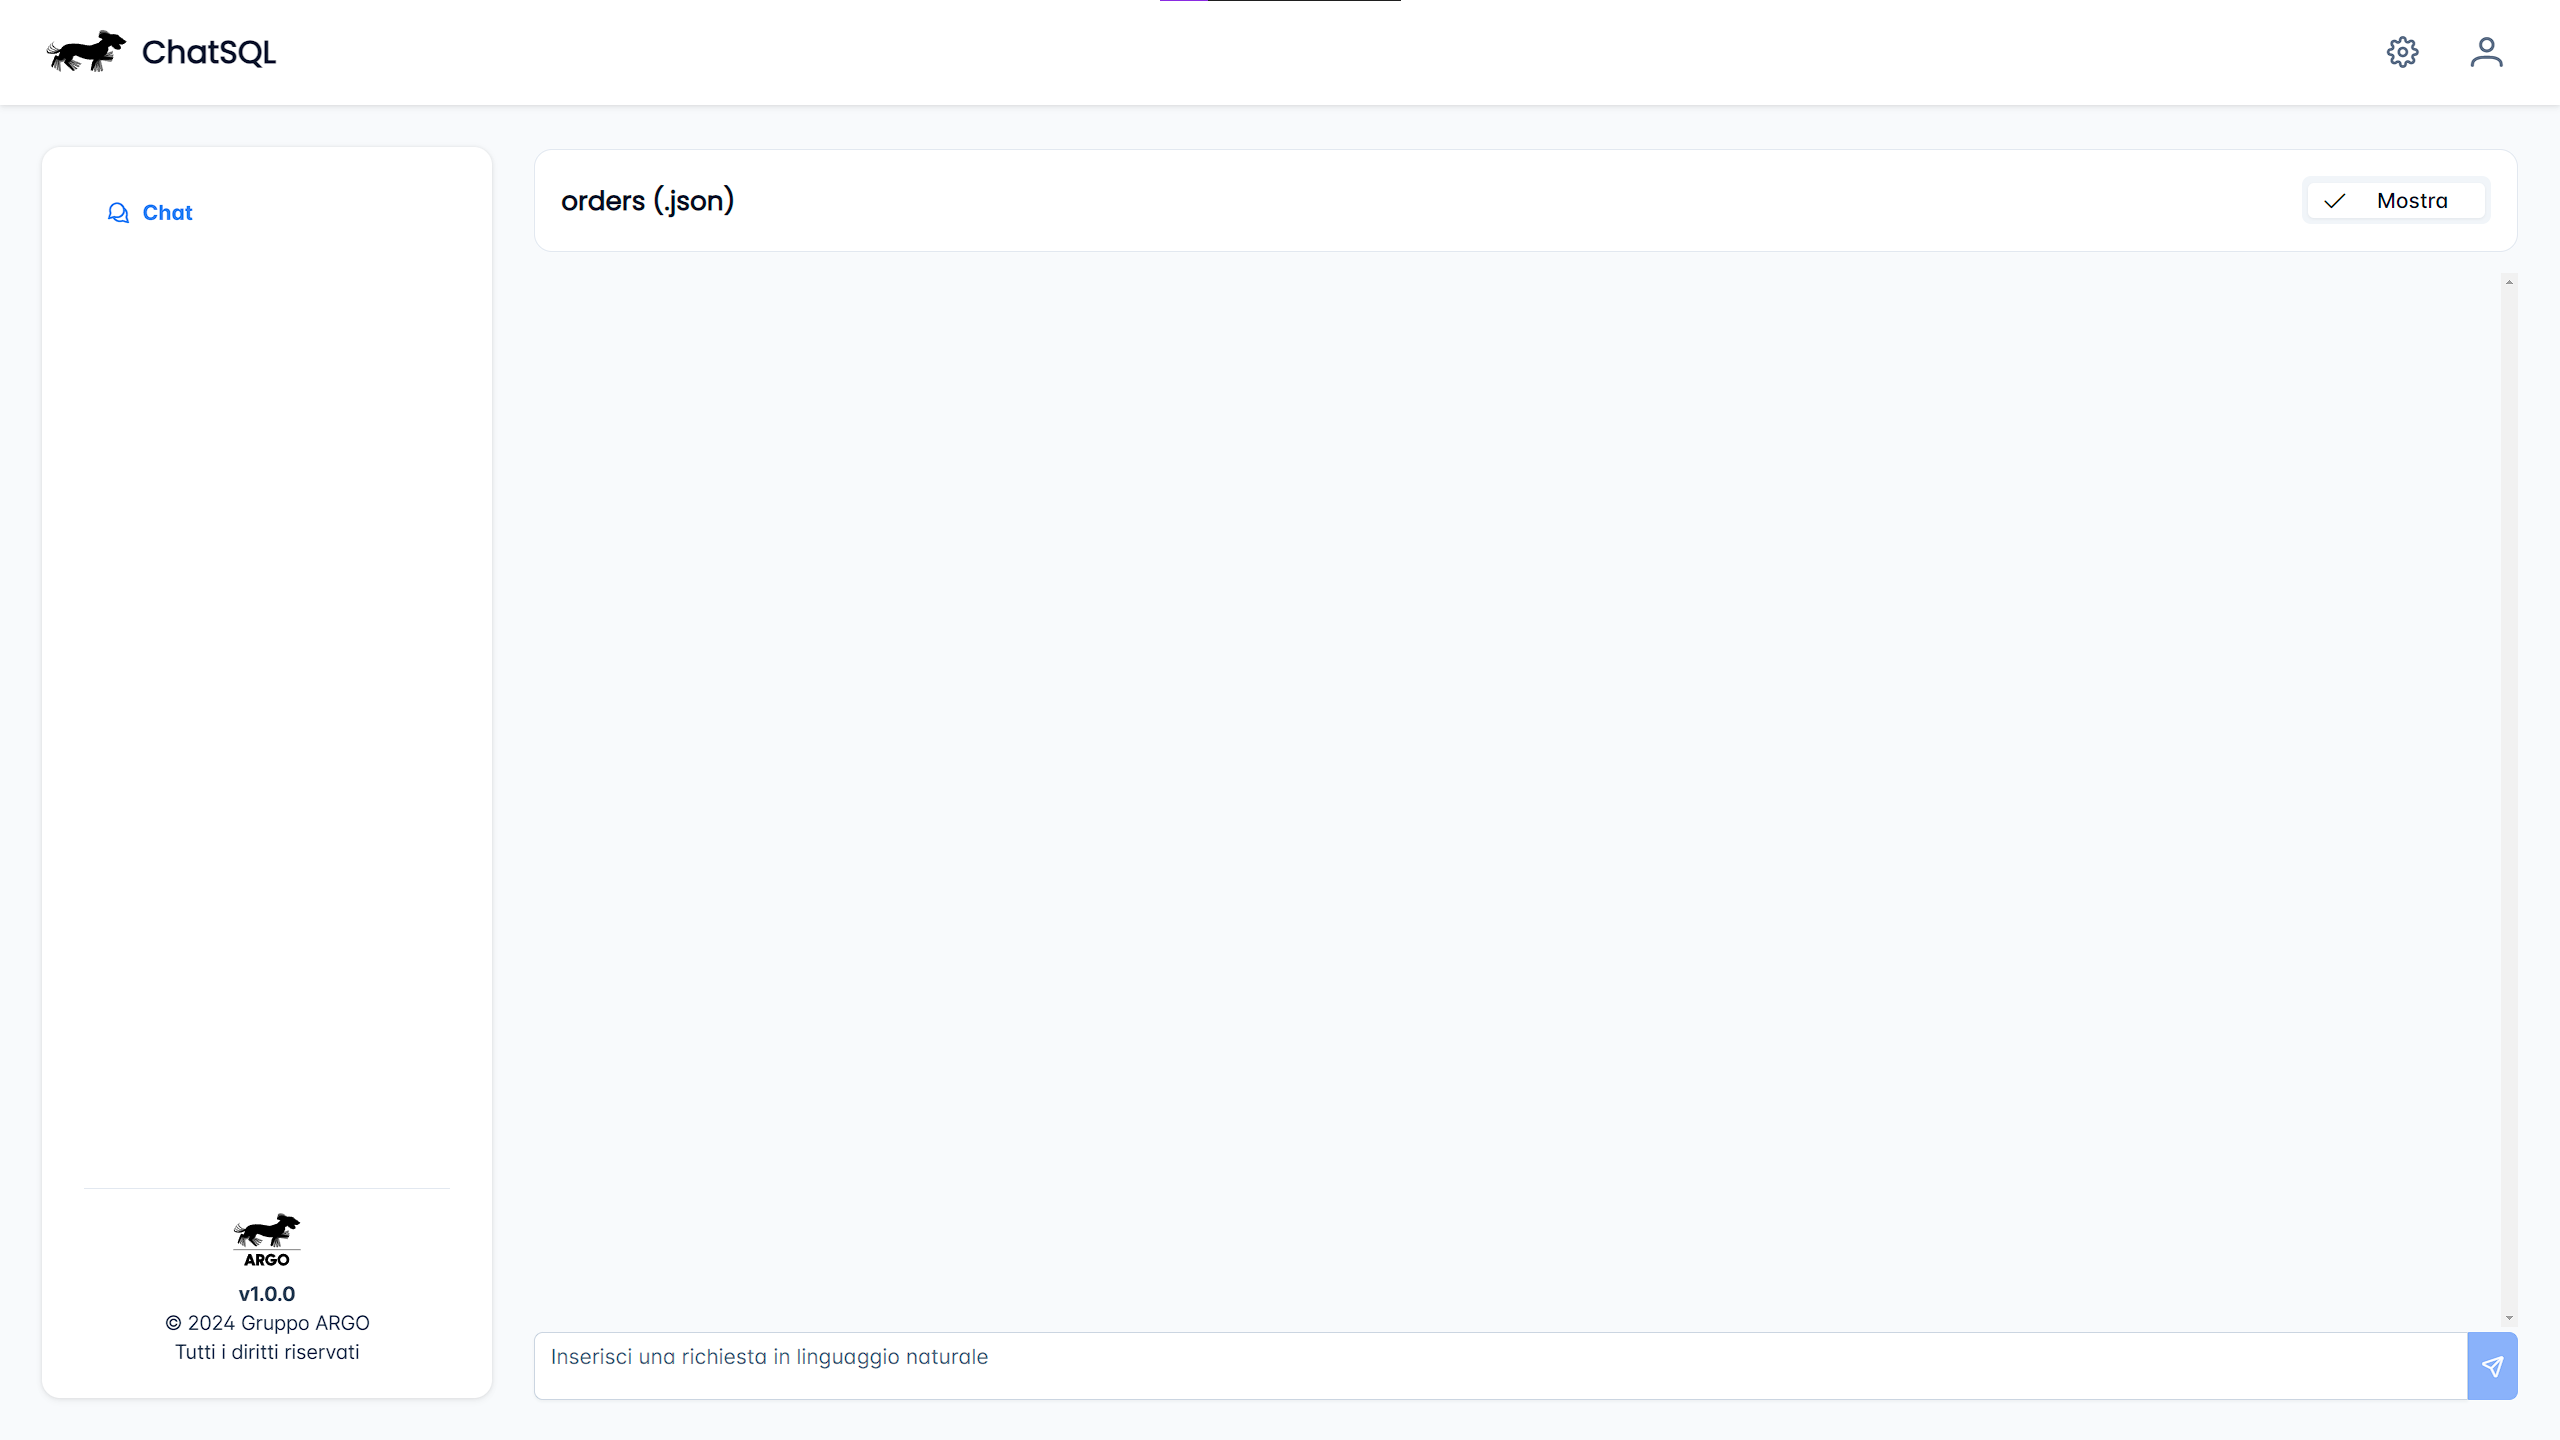
\includegraphics[width=65mm]{assets/workflow_1.png} &   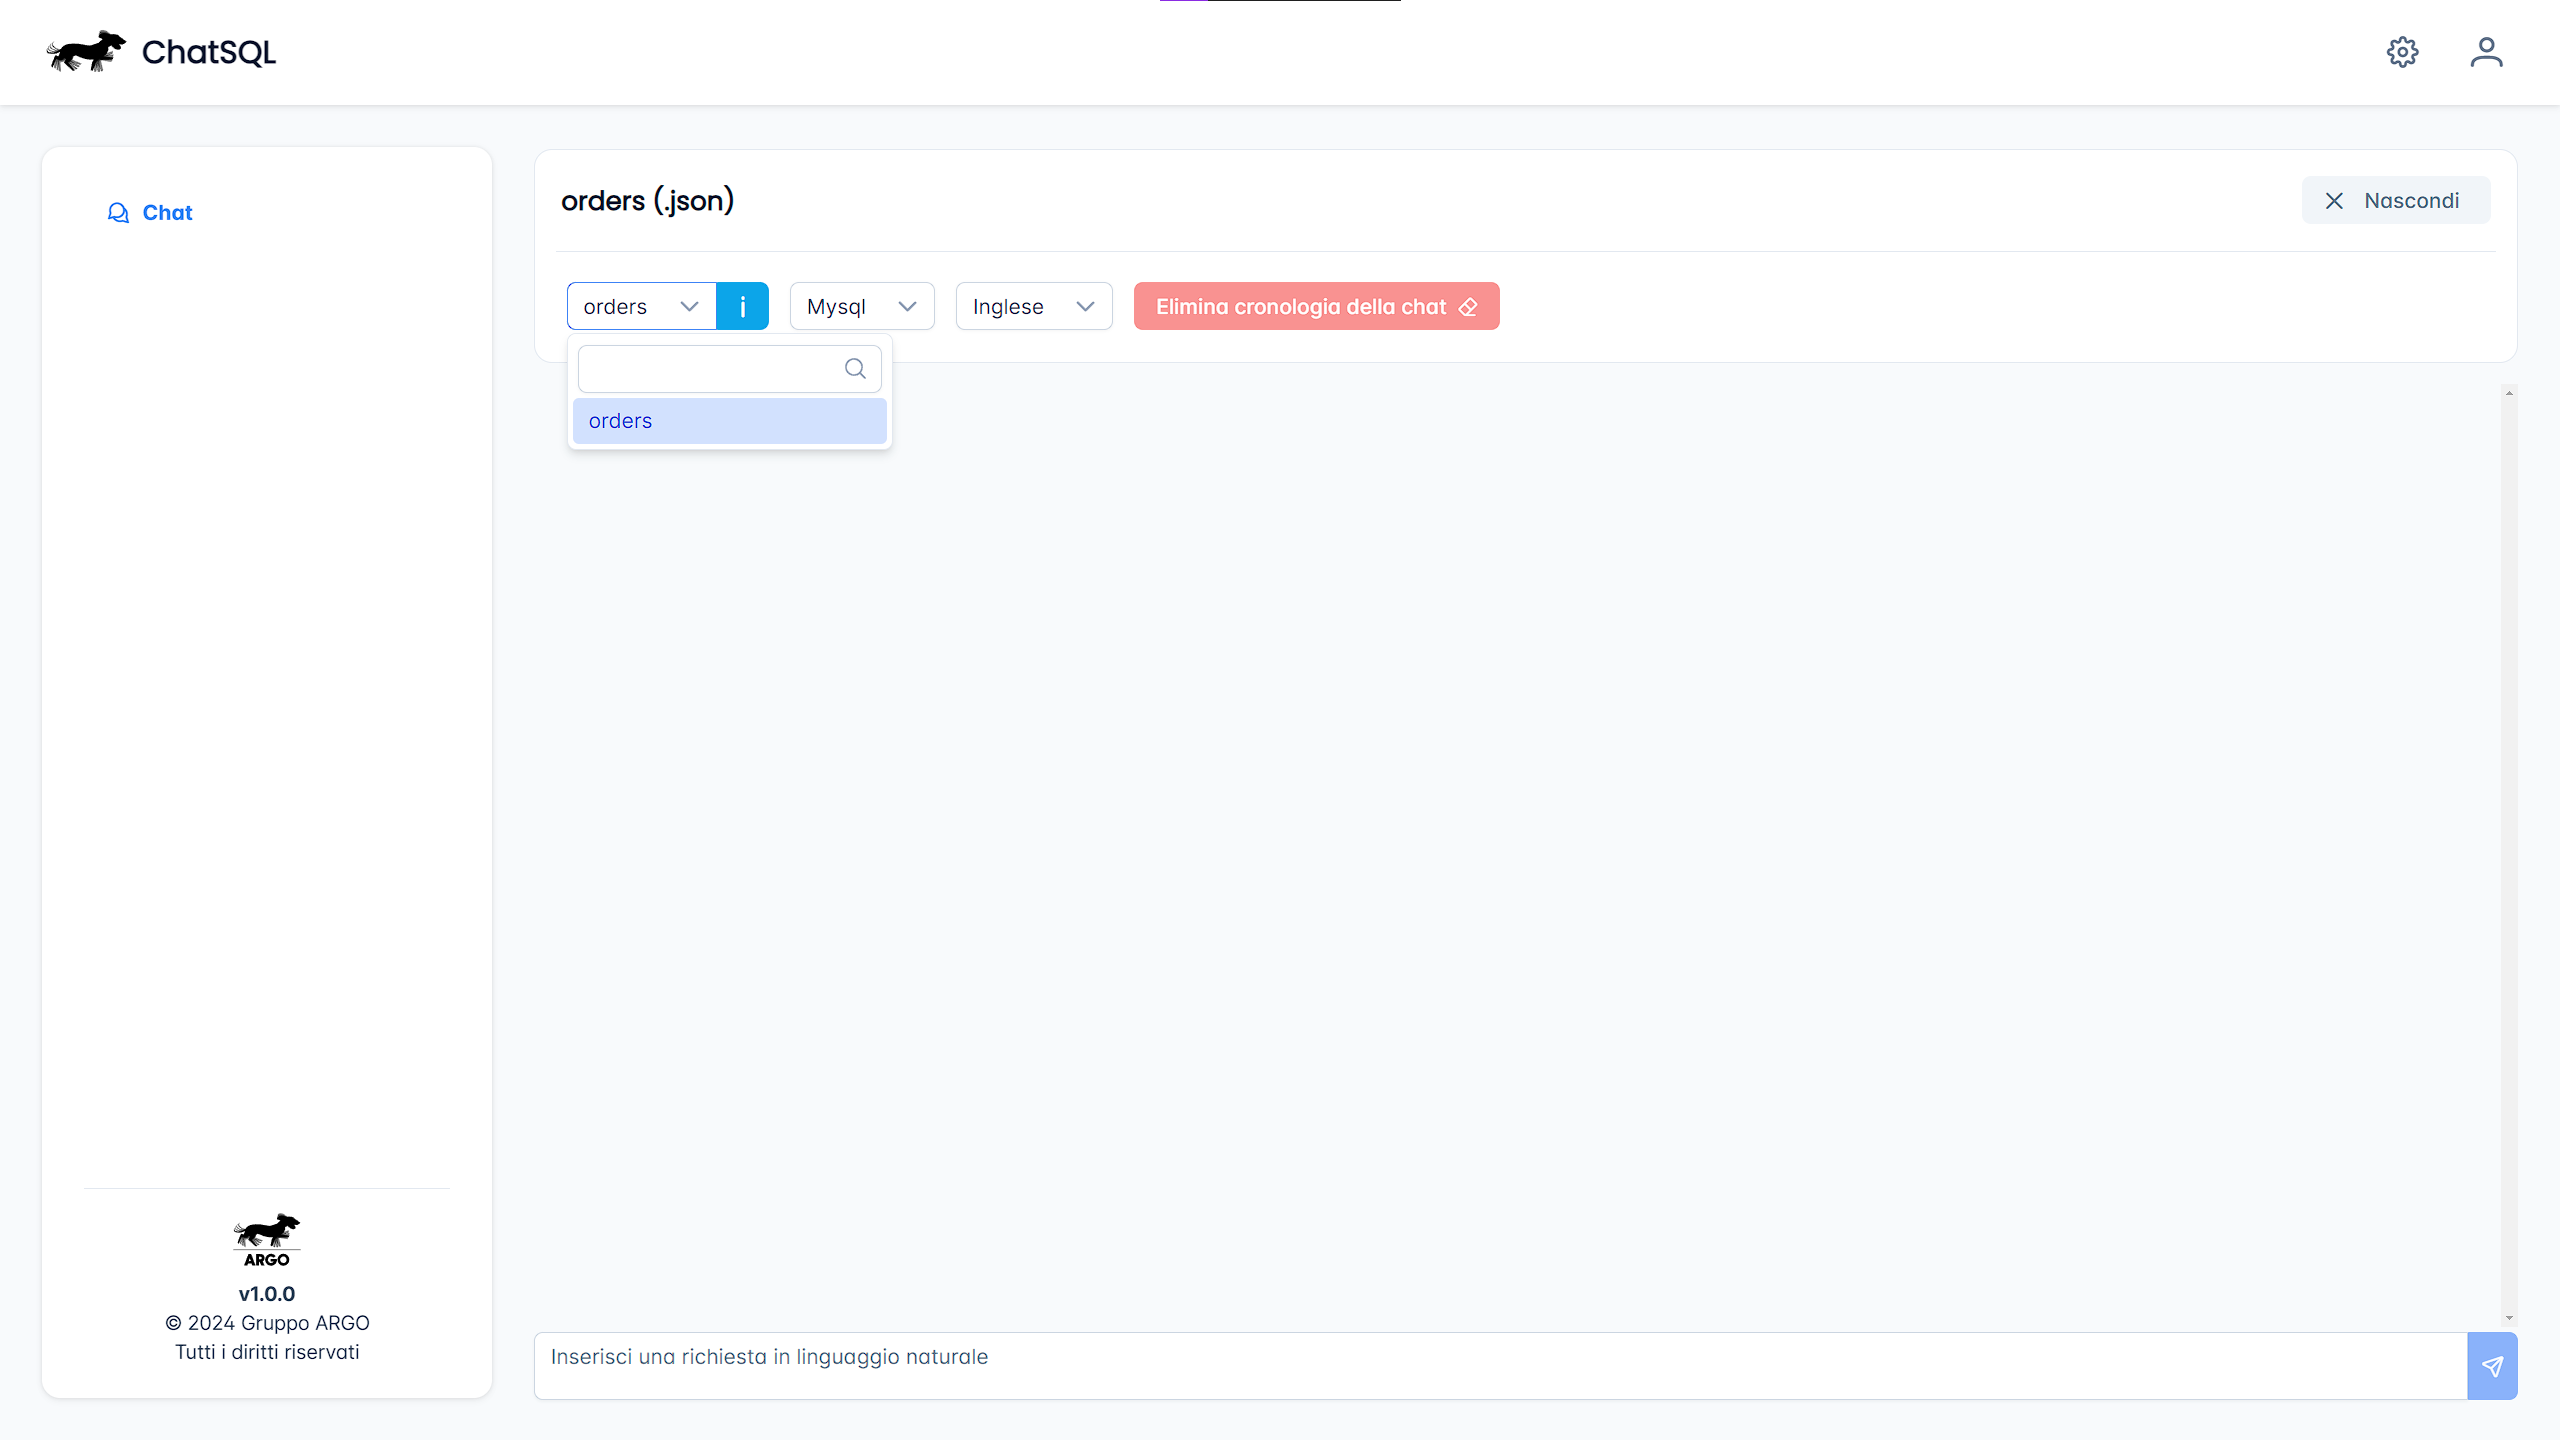
\includegraphics[width=65mm]{assets/workflow_2.png} \\
    1 & 2 \\[6pt]
     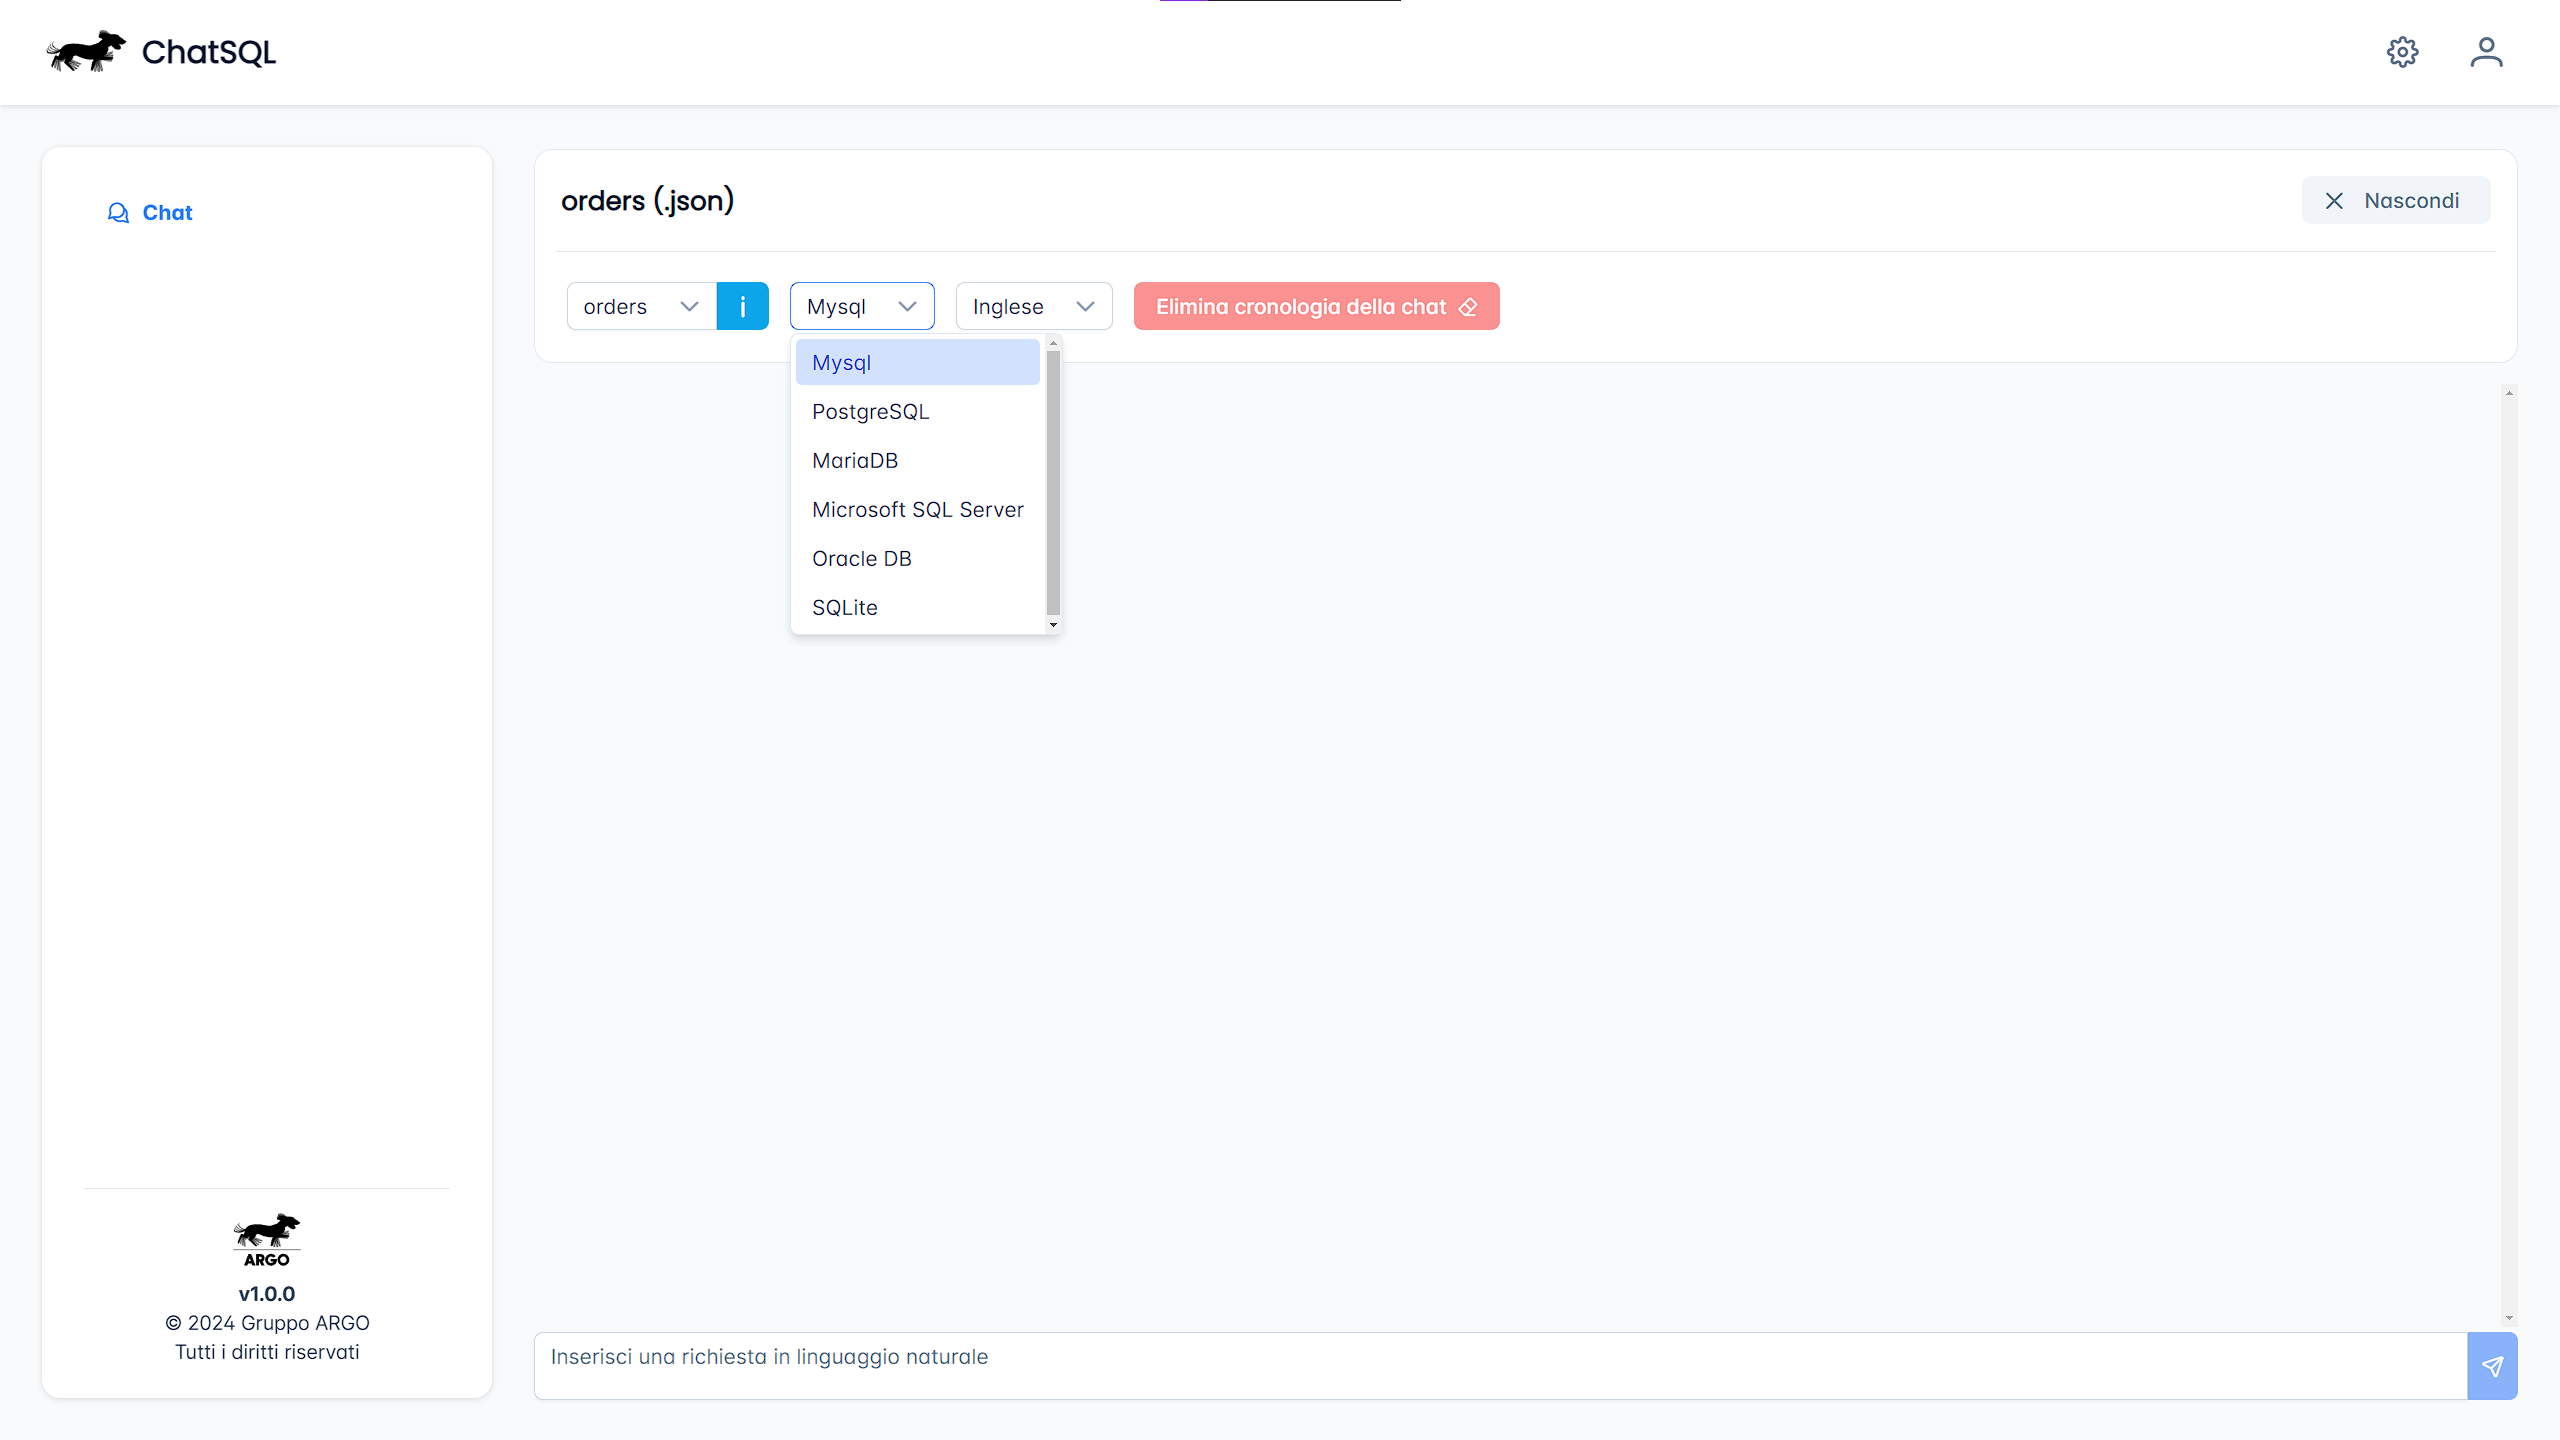
\includegraphics[width=65mm]{assets/workflow_3.png} &   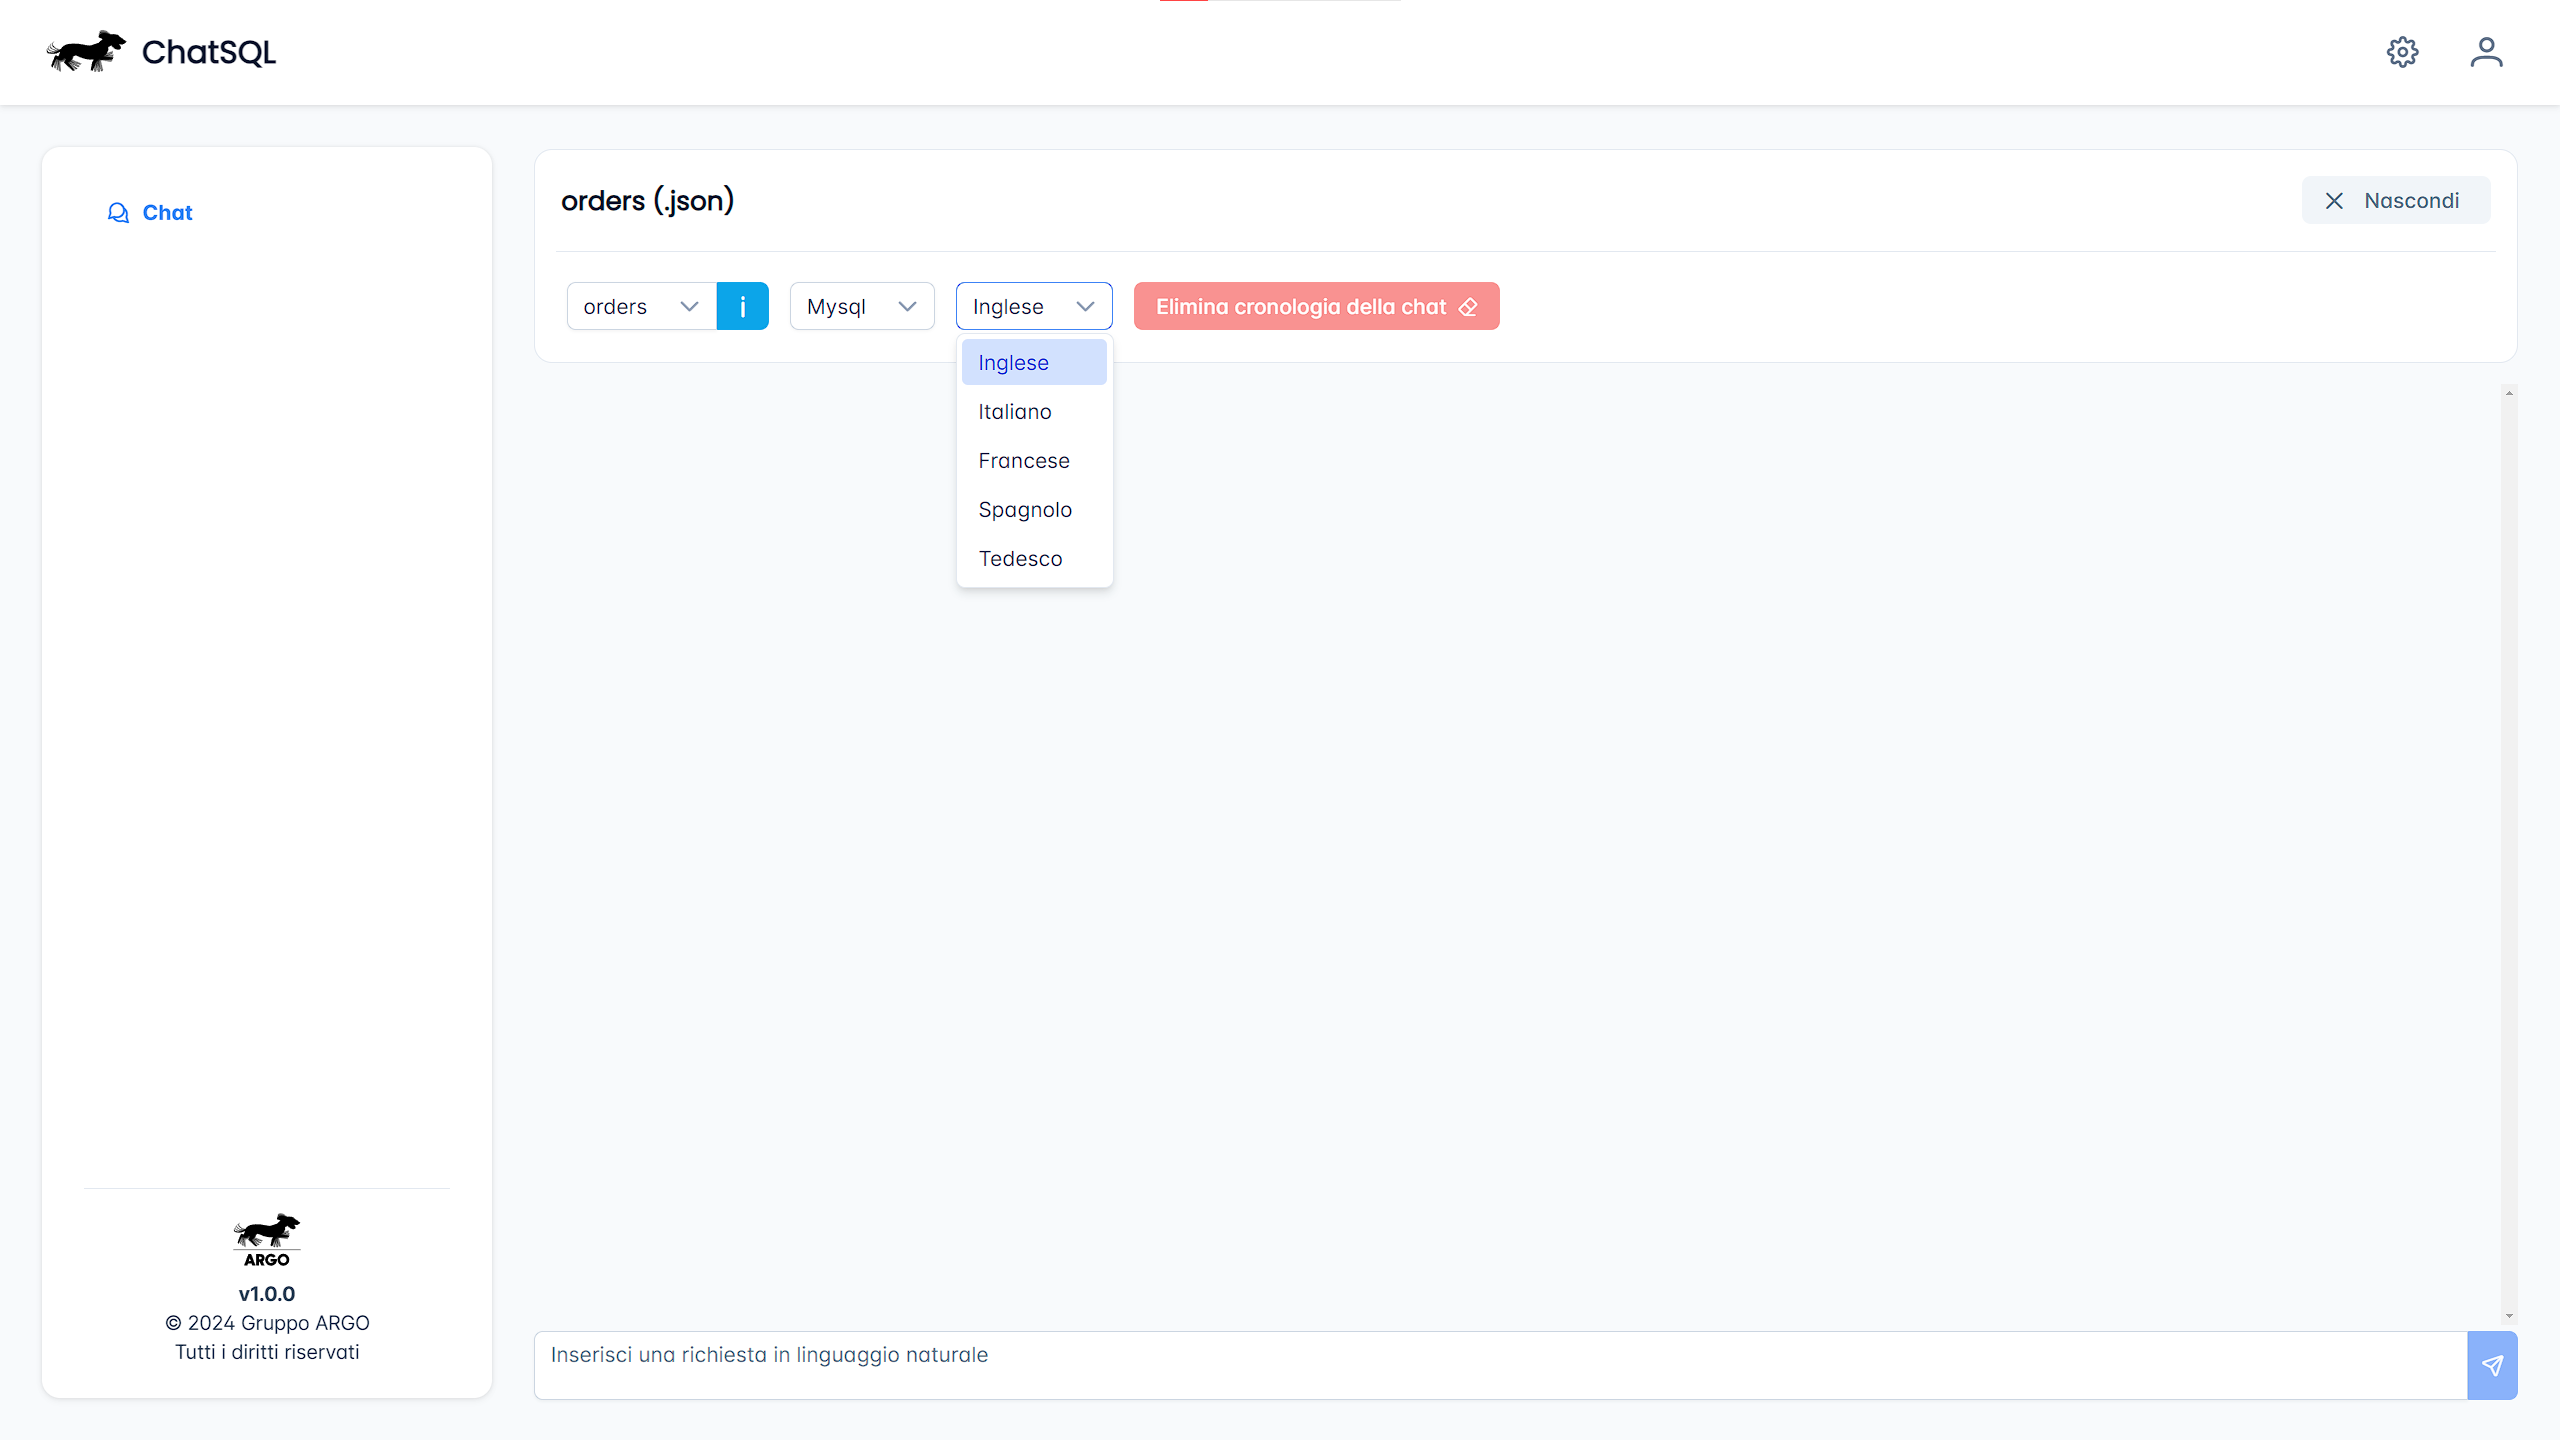
\includegraphics[width=65mm]{assets/workflow_4.png} \\
    3 & 4 \\[6pt]
   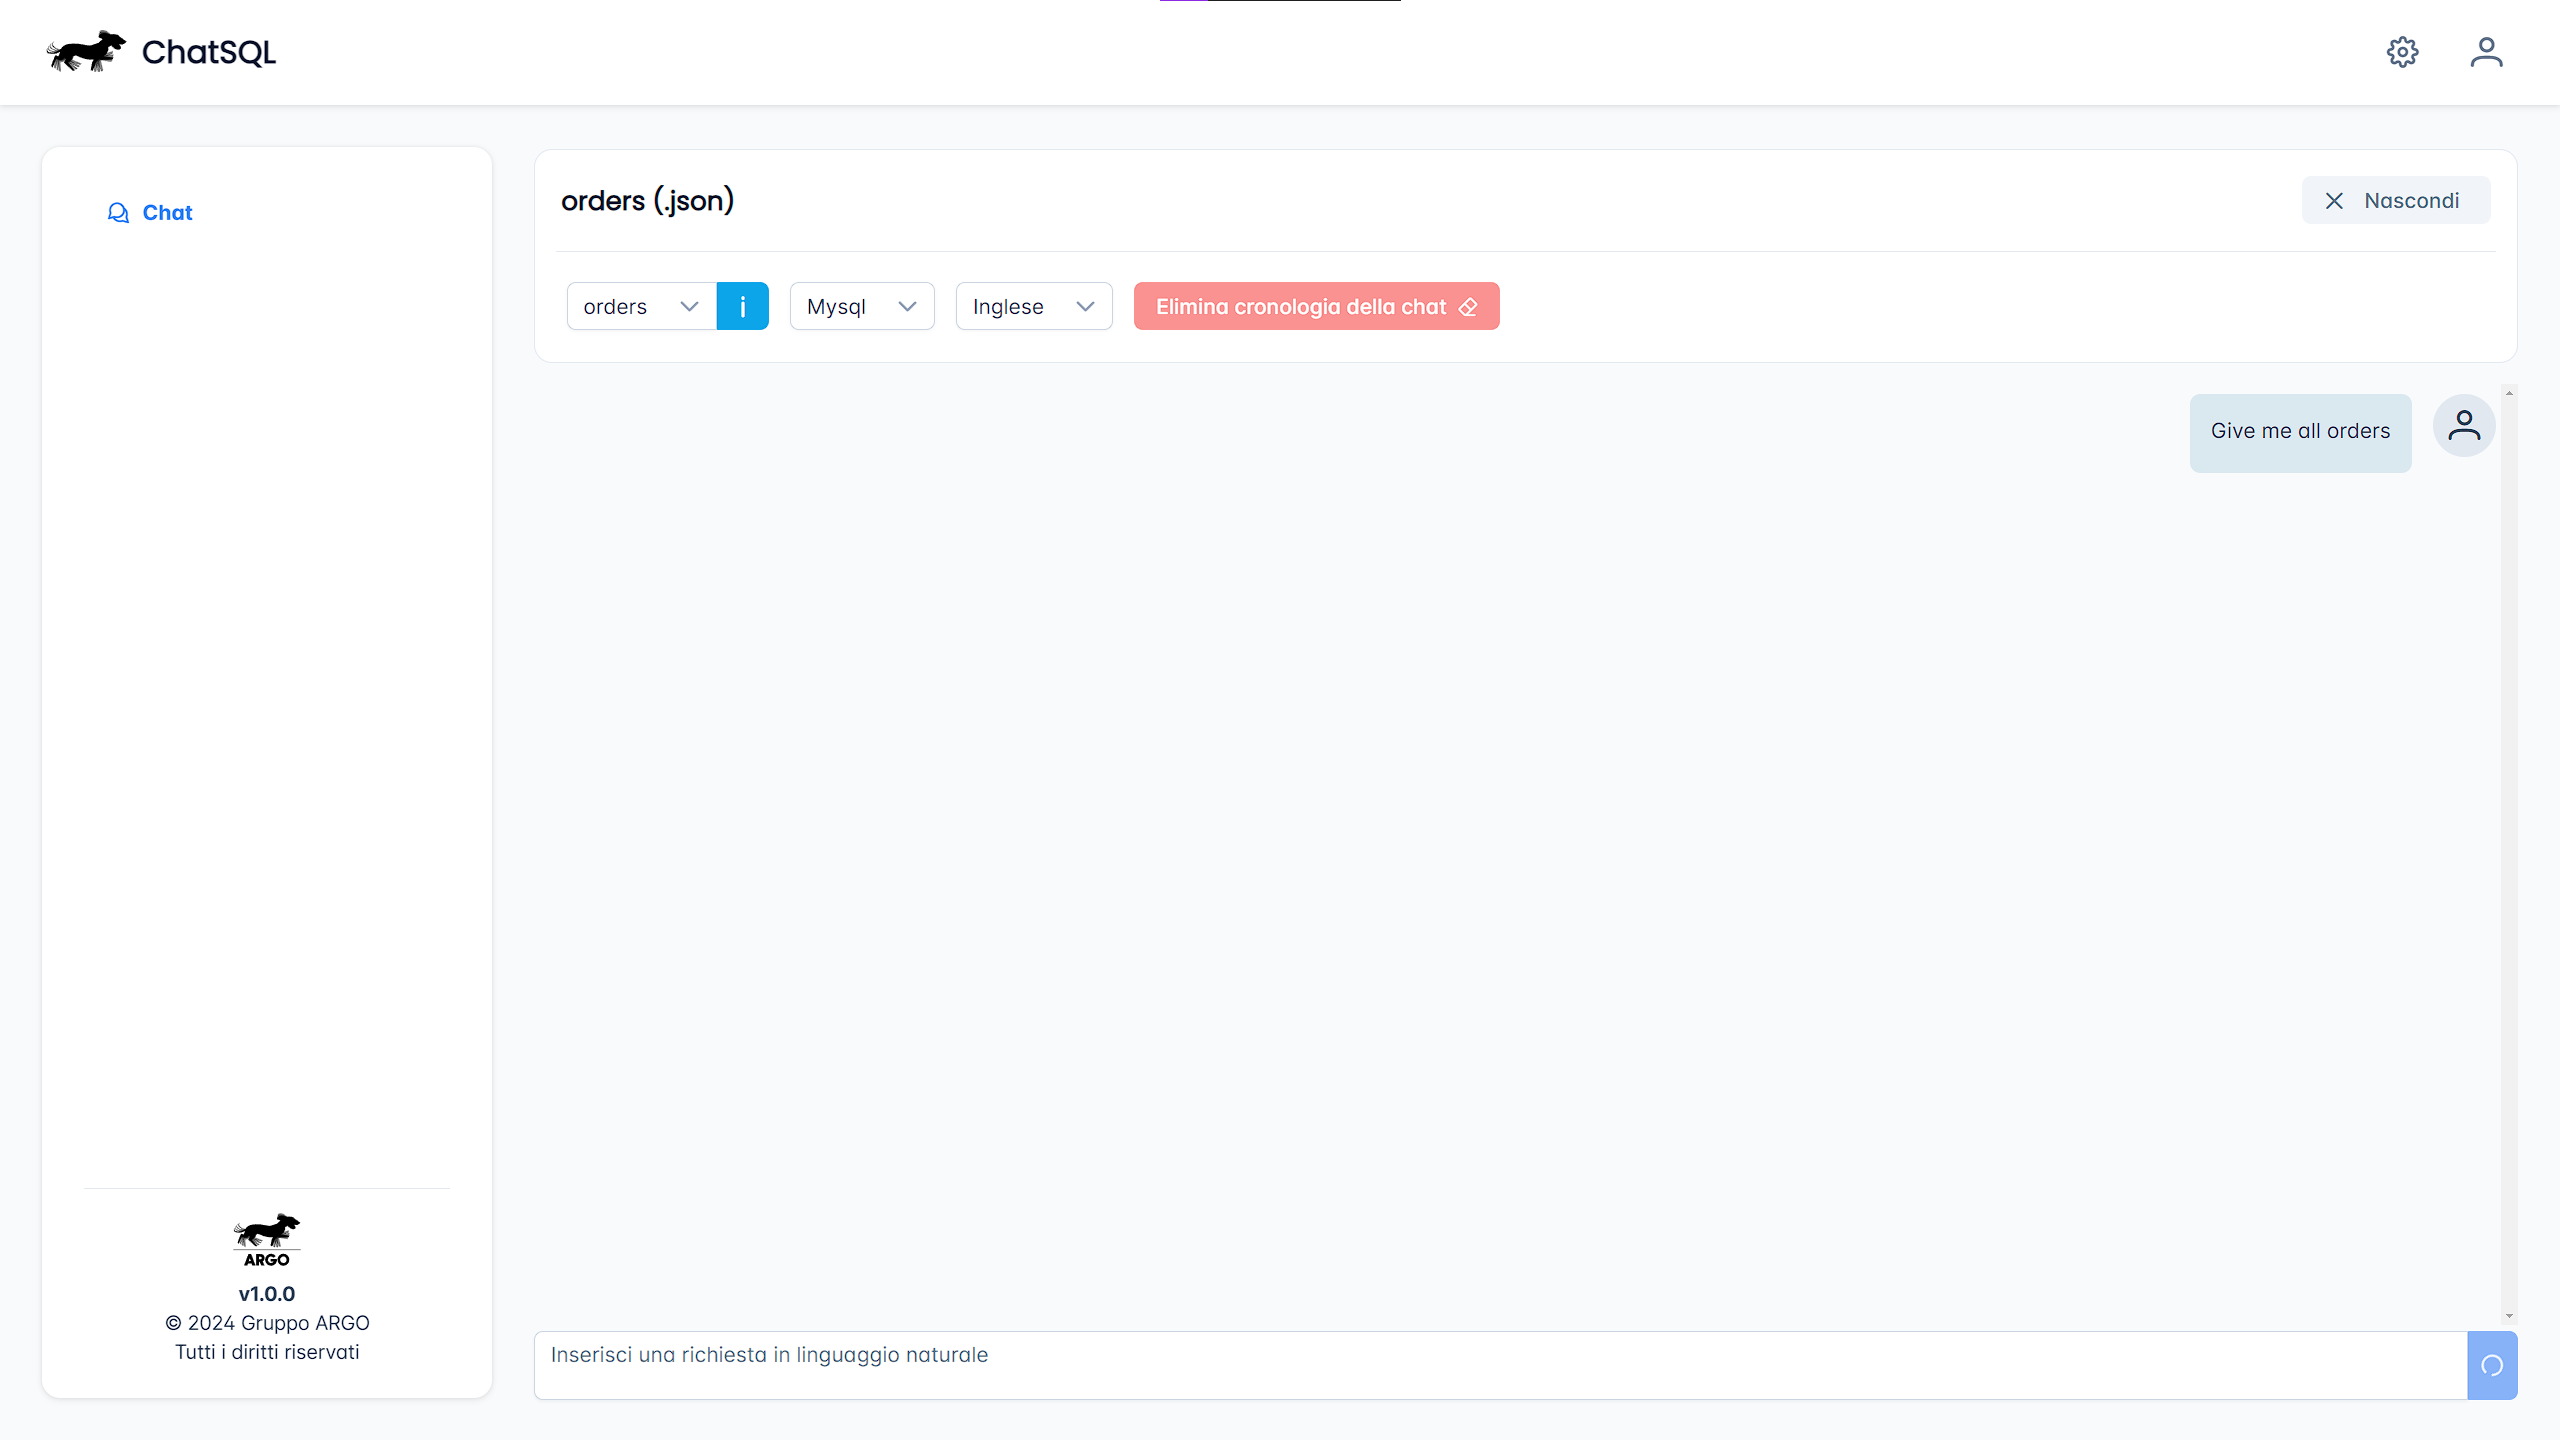
\includegraphics[width=65mm]{assets/workflow_5.png} &   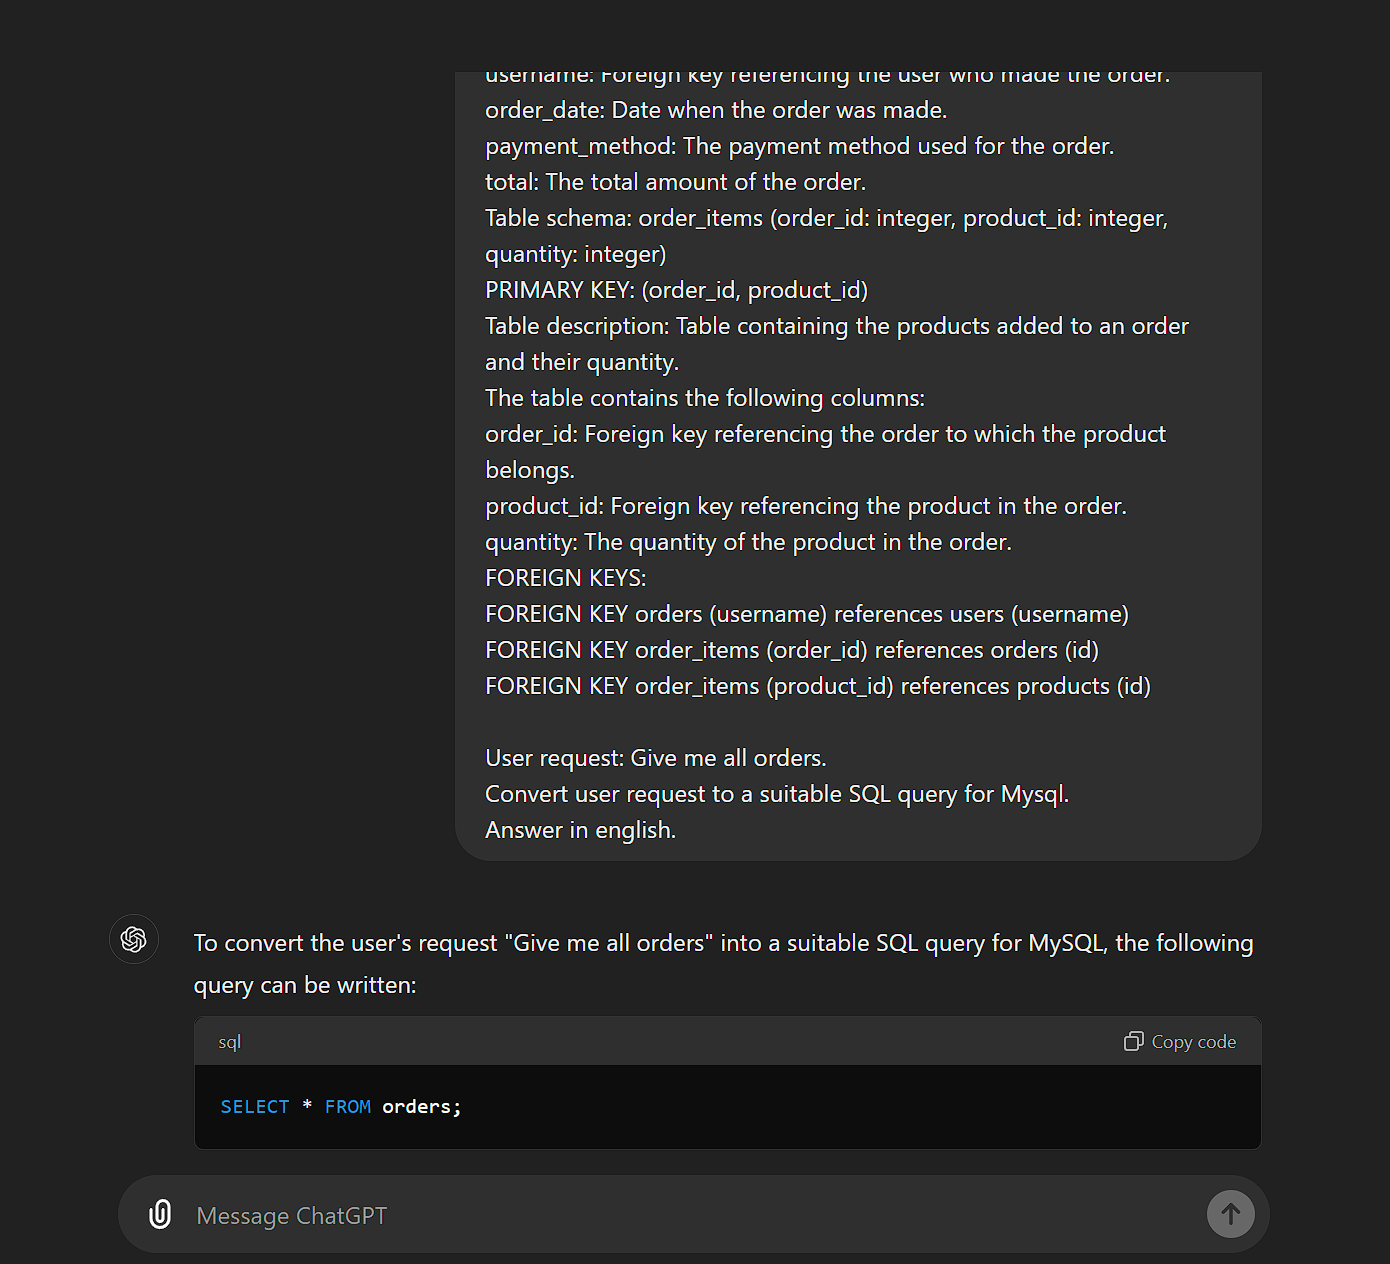
\includegraphics[width=65mm]{assets/workflow_6.png} \\
    5 & 6 \\[6pt]
    \multicolumn{2}{c}{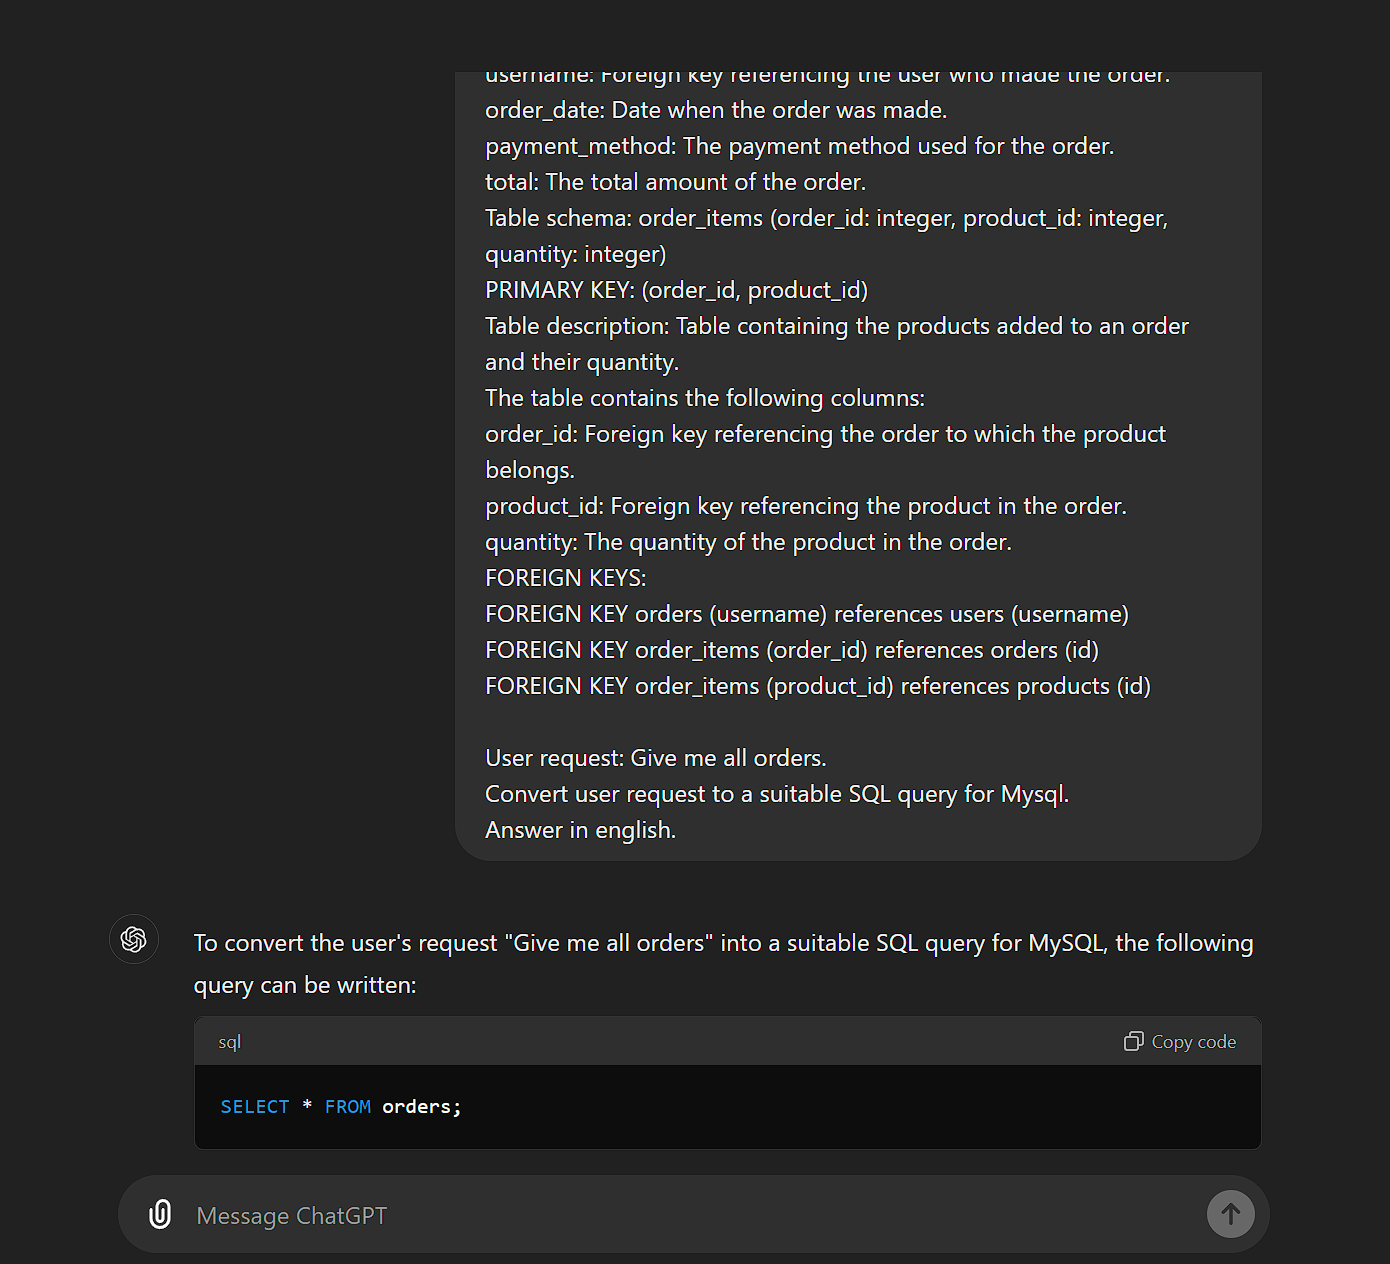
\includegraphics[width=65mm]{assets/workflow_7.png}}\\
    \multicolumn{2}{c}{7}
  \end{tabular}}
  \caption{Workflow per ottenere una query SQL}
\end{figure}
\par L'output atteso dal modello LLM è una query SQL che soddisfa la richiesta inserita, che potrà essere eseguita su un DBMS per ottenere i risultati desiderati.
\subsection{Sezione Tecnico}
\label{sec:sezTecnico}

\subsubsection*{Avviso}
\par Per accedere alle funzionalità del Tecnico, è necessario effettuare il login con successo. Le credenziali di accesso sono:
\begin{itemize}
    \item \textbf{Nome utente} (username): admin;
    \item \textbf{Password}: admin. 
\end{itemize}

\subsubsection{Autenticazione} \label{sec:autenticazione}
\par Nella sezione superiore destra dell'interfaccia, cliccando sull'icona di login 
\includegraphics[height=1.2em]{assets/user_icon.png}, l'Utente può inserire le credenziali per sbloccare le funzionalità del Tecnico.

\begin{figure}[H]
  \centering
  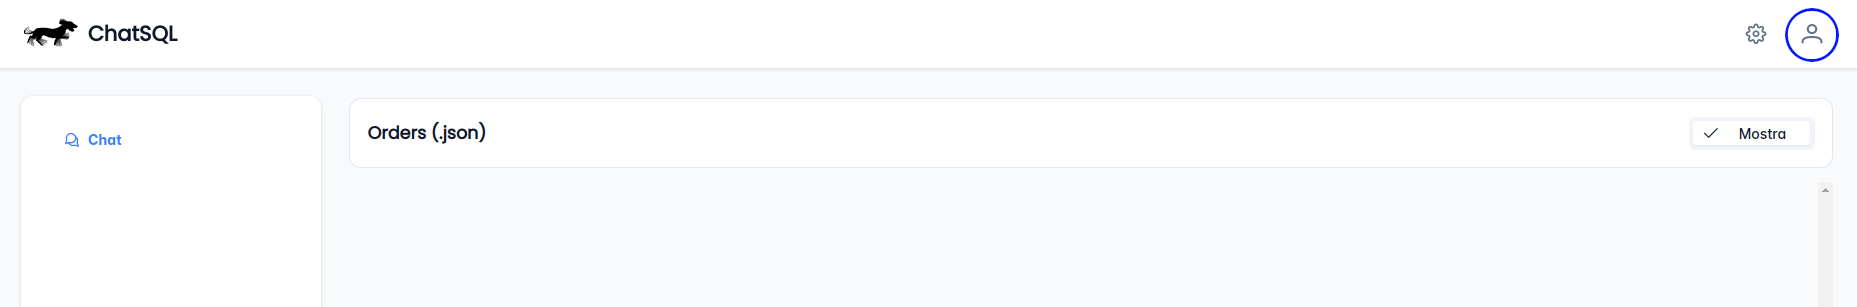
\includegraphics[width=\textwidth]{assets/login_topbar.png}
  \caption{Topbar con menu di autenticazione}
\end{figure}
\begin{figure}[H]
  \centering
  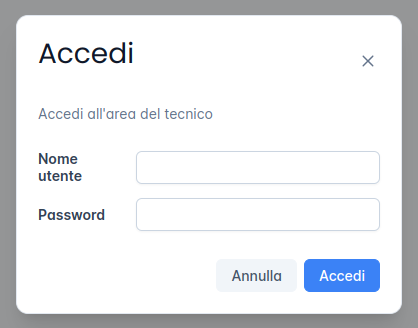
\includegraphics[width=0.50\textwidth]{assets/login_modal.png}
  \caption{Modale di login}
\end{figure}

\subsubsection{Gestione dizionari}
\par La schermata sottostante mostra l'elenco completo dei \glossario{dizionari dati} caricati nell'applicazione. Per ciascun dizionario, il sistema fornisce dei pulsanti per eseguire operazioni su di esso.
\begin{figure}[H]
  \centering
  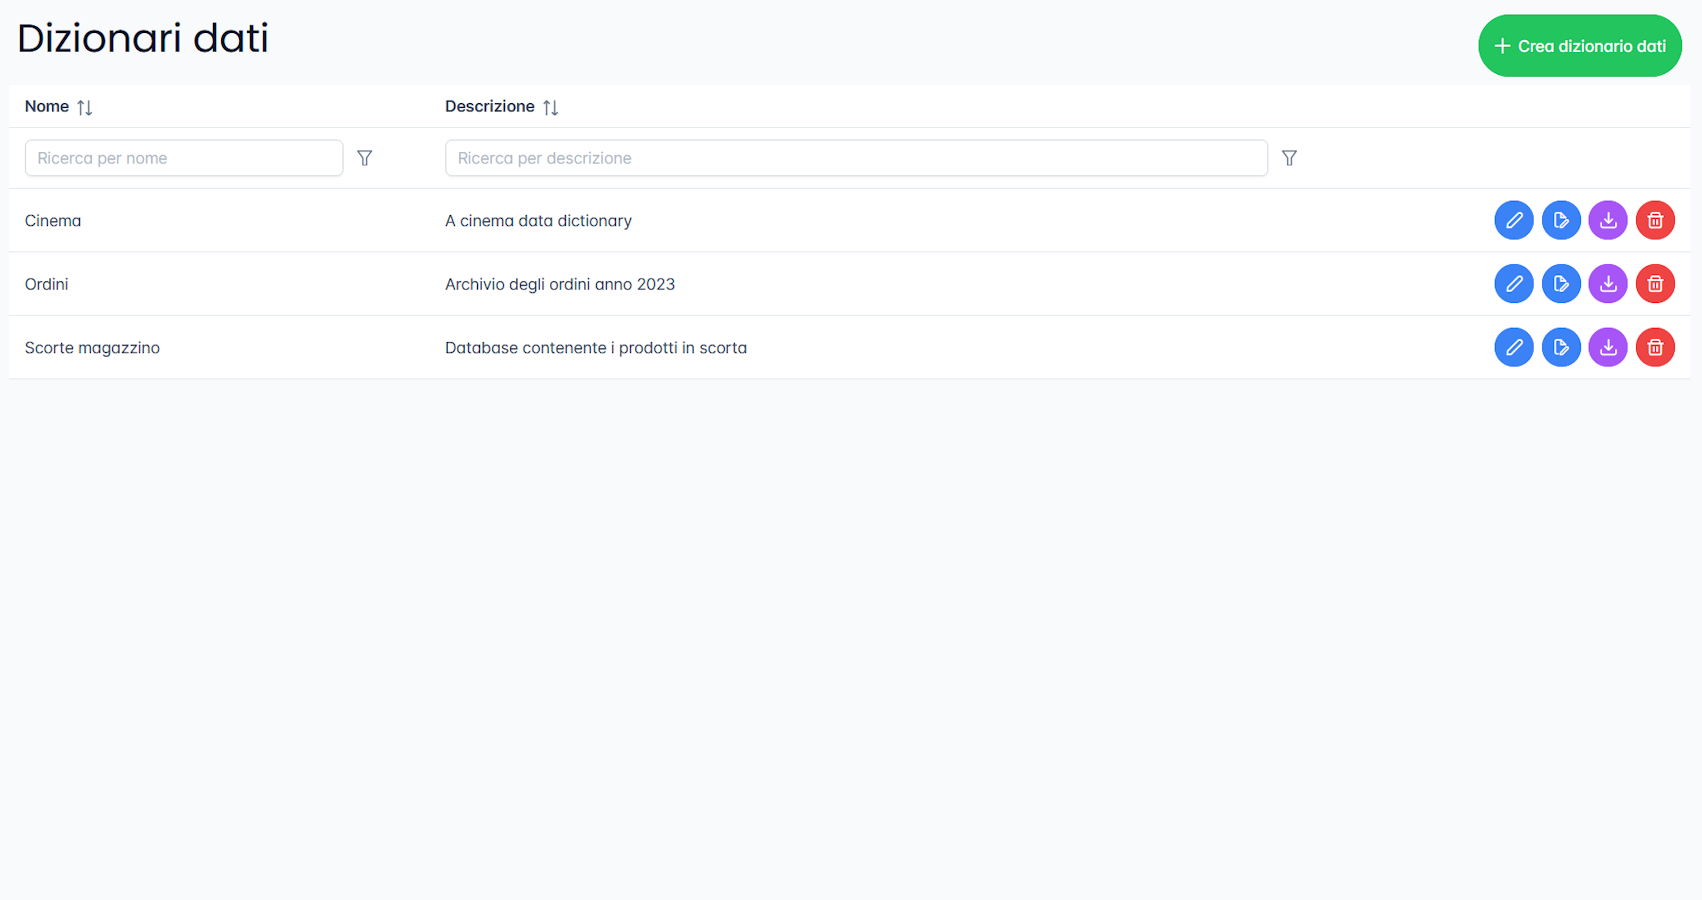
\includegraphics[width=1\textwidth]{assets/dd_list.png}
  \caption{Schermata di gestione dizionari dati}
\end{figure}

\subsubsubsection{Ricerca dizionari dati}
\par Il Tecnico può filtrare i dizionari per nome e descrizione utilizzando due campi di testo all'interno della tabella. La ricerca viene eseguita in tempo reale, mostrando immediatamente i risultati.

\subsubsubsection{Inserimento dizionario dati}
\par Cliccando sul pulsante "Crea dizionario dati" 
\includegraphics[height=1.2em]{assets/dd_create_button.png}, il sistema apre una finestra modale in cui è possibile inserire i parametri per creare un nuovo \glossario{dizionario dati}:
\begin{figure}[H]
  \centering
  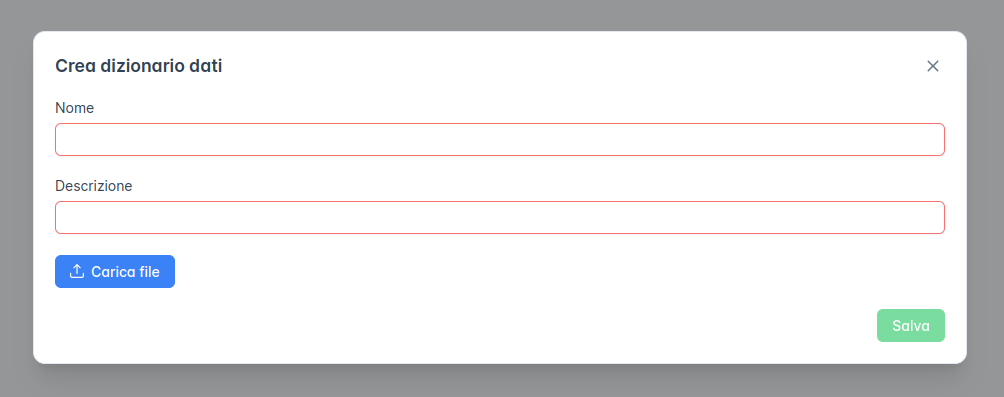
\includegraphics[width=0.5\textwidth]{assets/dd_modal_create.png}
  \caption{Modale di creazione dizionario dati}
\end{figure}
\begin{itemize}
  \item \textbf{Nome}: deve essere univoco rispetto agli altri dizionari;
  \item \textbf{Descrizione}: stringa testuale che descrive brevemente il dizionario;
  \item \textbf{File}: deve essere un file in formato \glossario{JSON}, di dimensione massima 1 MB e strutturato secondo il modello proposto.
\end{itemize}
\vspace{0.5\baselineskip}
\par Una volta salvato, il dizionario verrà aggiunto all'elenco.

\subsubsubsection{Aggiornamento dizionario dati}
\par Cliccando sul pulsante di aggiornamento dei metadati 
\includegraphics[height=1.2em]{assets/dd_edit_metadata_button.png}, il sistema apre una finestra modale in cui è possibile modificare i seguenti parametri:
\begin{itemize}
  \item \textbf{Nome}: deve essere univoco rispetto agli altri dizionari;
  \item \textbf{Descrizione}: stringa testuale che descrive brevemente il dizionario.
\end{itemize}

\subsubsubsection{Modifica file di configurazione dizionario dati}
\par Cliccando sul pulsante di modifica del file di configurazione di un \glossario{dizionario dati} 
\includegraphics[height=1.2em]{assets/dd_edit_button.png}, il sistema apre una finestra modale in cui è possibile caricare un nuovo file.

\subsubsubsection{Download file dizionario dati}
\par Cliccando sul pulsante di download 
\includegraphics[height=1.2em]{assets/dd_download_button.png}, verrà scaricato il file del \glossario{dizionario dati} corrispondente in formato \glossario{JSON}.

\subsubsubsection{Elimina file dizionario dati}
\par Cliccando sul pulsante di cancellazione 
\includegraphics[height=1.2em]{assets/dd_delete_button.png}, il sistema apre una finestra modale di conferma per l'eliminazione del \glossario{dizionario dati}.
\begin{figure}[H]
  \centering
  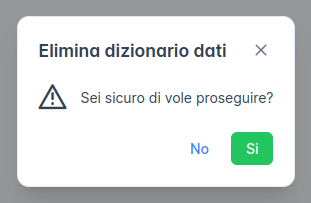
\includegraphics[width=0.5\textwidth]{assets/dd_confirm_delete.png}
  \caption{Modale di conferma eliminazione dizionario dati}
\end{figure}
\par In caso di conferma, il dizionario verrà eliminato dalla lista.

\subsubsection{Strumento di debug}

\subsubsubsection{Generazione del messaggio di debug}
\par Per il Tecnico è disponibile uno strumento di controllo per i meccanismi di generazione del \glossario{prompt} che aiuta a comprendere e analizzare i passaggi algoritmici che hanno prodotto il prompt restituito sulla base di una interrogazione. Il \glossario{debug} assiste il Tecnico nella fase di miglioramento del \glossario{dizionario dati}, poiché fornisce una panoramica dell'interazione tra i modelli di intelligenza artificiale e il dizionario stesso. L'obiettivo di questa funzionalità è individuare le aree del dizionario dati che necessitano di aggiornamenti, con particolare attenzione alle descrizioni in linguaggio naturale di tabelle e colonne.

\par Per utilizzare questa funzionalità, il Tecnico deve inserire un messaggio nell'apposita maschera di richiesta all'interno della chat (\sezione{sec:interazione-chat}). Una volta ottenuto il prompt, è necessario cliccare sull'icona del punto interrogativo in alto a destra, da cui si aprirà un'altra finestra sovrapposta a quella attuale.

\begin{figure}[H]
  \centering
  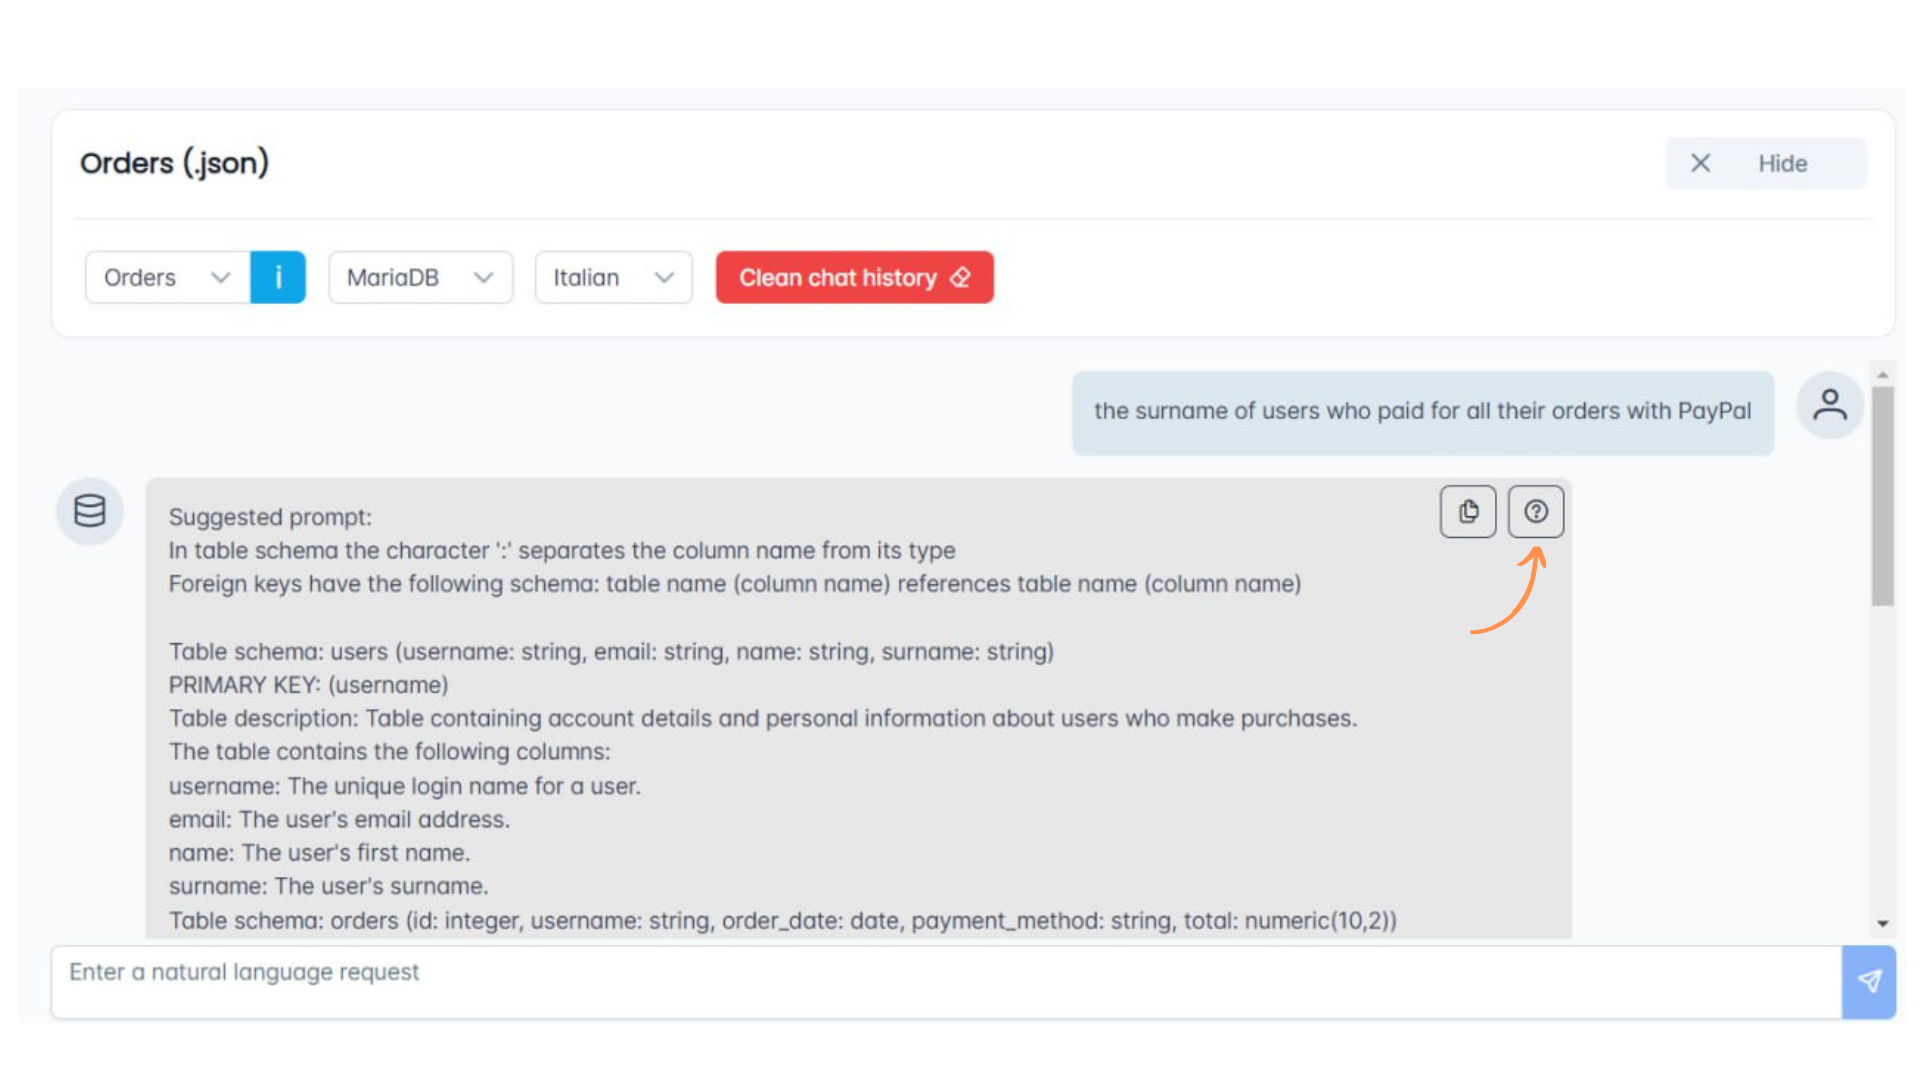
\includegraphics[width=\textwidth]{assets/tasto_info_debug.png}
  \caption{Selezione funzionalità di debug}
\end{figure}

\par Nel messaggio di debug è documentato il modo in cui le descrizioni interagiscono con il modello di \glossario{AI}. In ordine verranno visualizzate le seguenti informazioni: 
\begin{itemize}
  \item Data e ora di generazione del \glossario{log}; 
  \item La richiesta inserita in linguaggio naturale;
  \item Analisi della prima fase di generazione del prompt con una lista delle tabelle considerate rilevanti dal modello, di cui si riportano le seguenti informazioni:
  \begin{itemize}
    \item Nome della tabella;
    \item Punteggio assegnato alla tabella;
    \item Descrizione della tabella;
    \item Classifica di importanza dei termini presenti nella descrizione della tabella;
    \item Descrizione della colonna più rilevante;
    \item Classifica di importanza dei termini presenti nella descrizione della colonna.
  \end{itemize}
  \item Analisi della seconda fase di generazione del prompt con una lista delle tabelle pertinenti, di cui viene indicato il motivo per cui sono state inserite o meno nel prompt finale.
\end{itemize}
\begin{figure}[H]
  \centering
  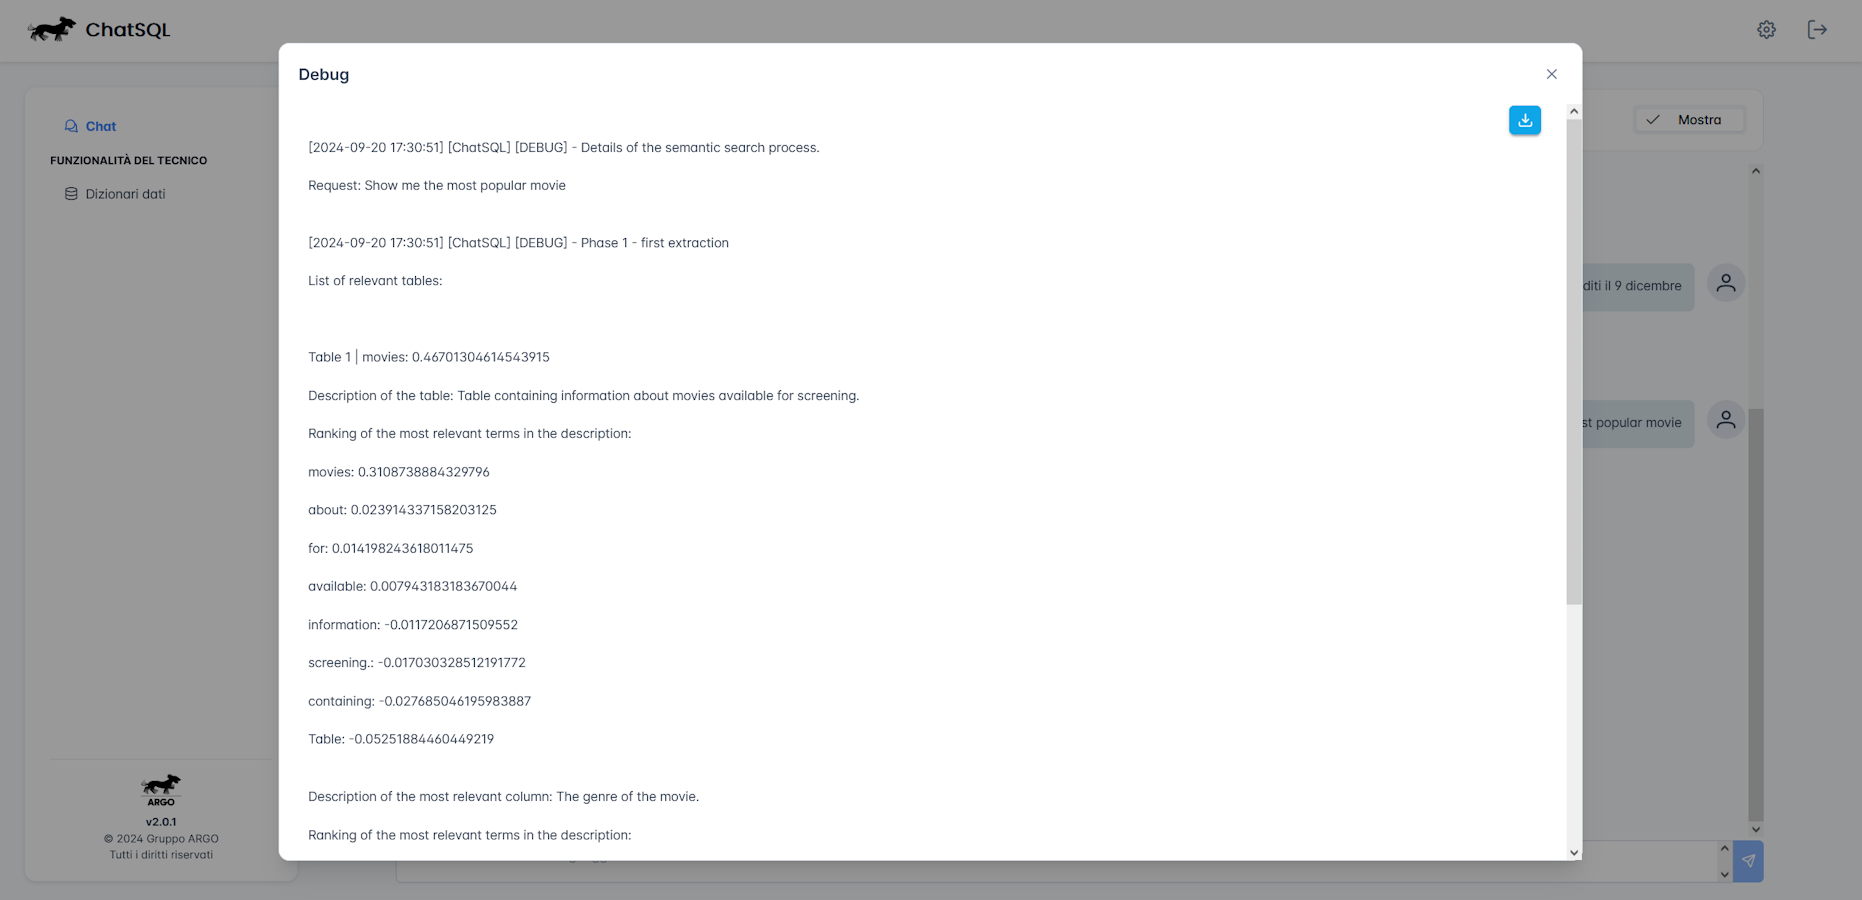
\includegraphics[width=\textwidth]{assets/analisi_debug.png}
  \caption{Esempio di messaggio di debug}
\end{figure}

\par Cliccando sul pulsante di chiusura in alto a destra, il modale di debug verrà nascosto e sarà possibile visualizzare nuovamente il prompt generato.
\begin{figure}[H]
  \centering
  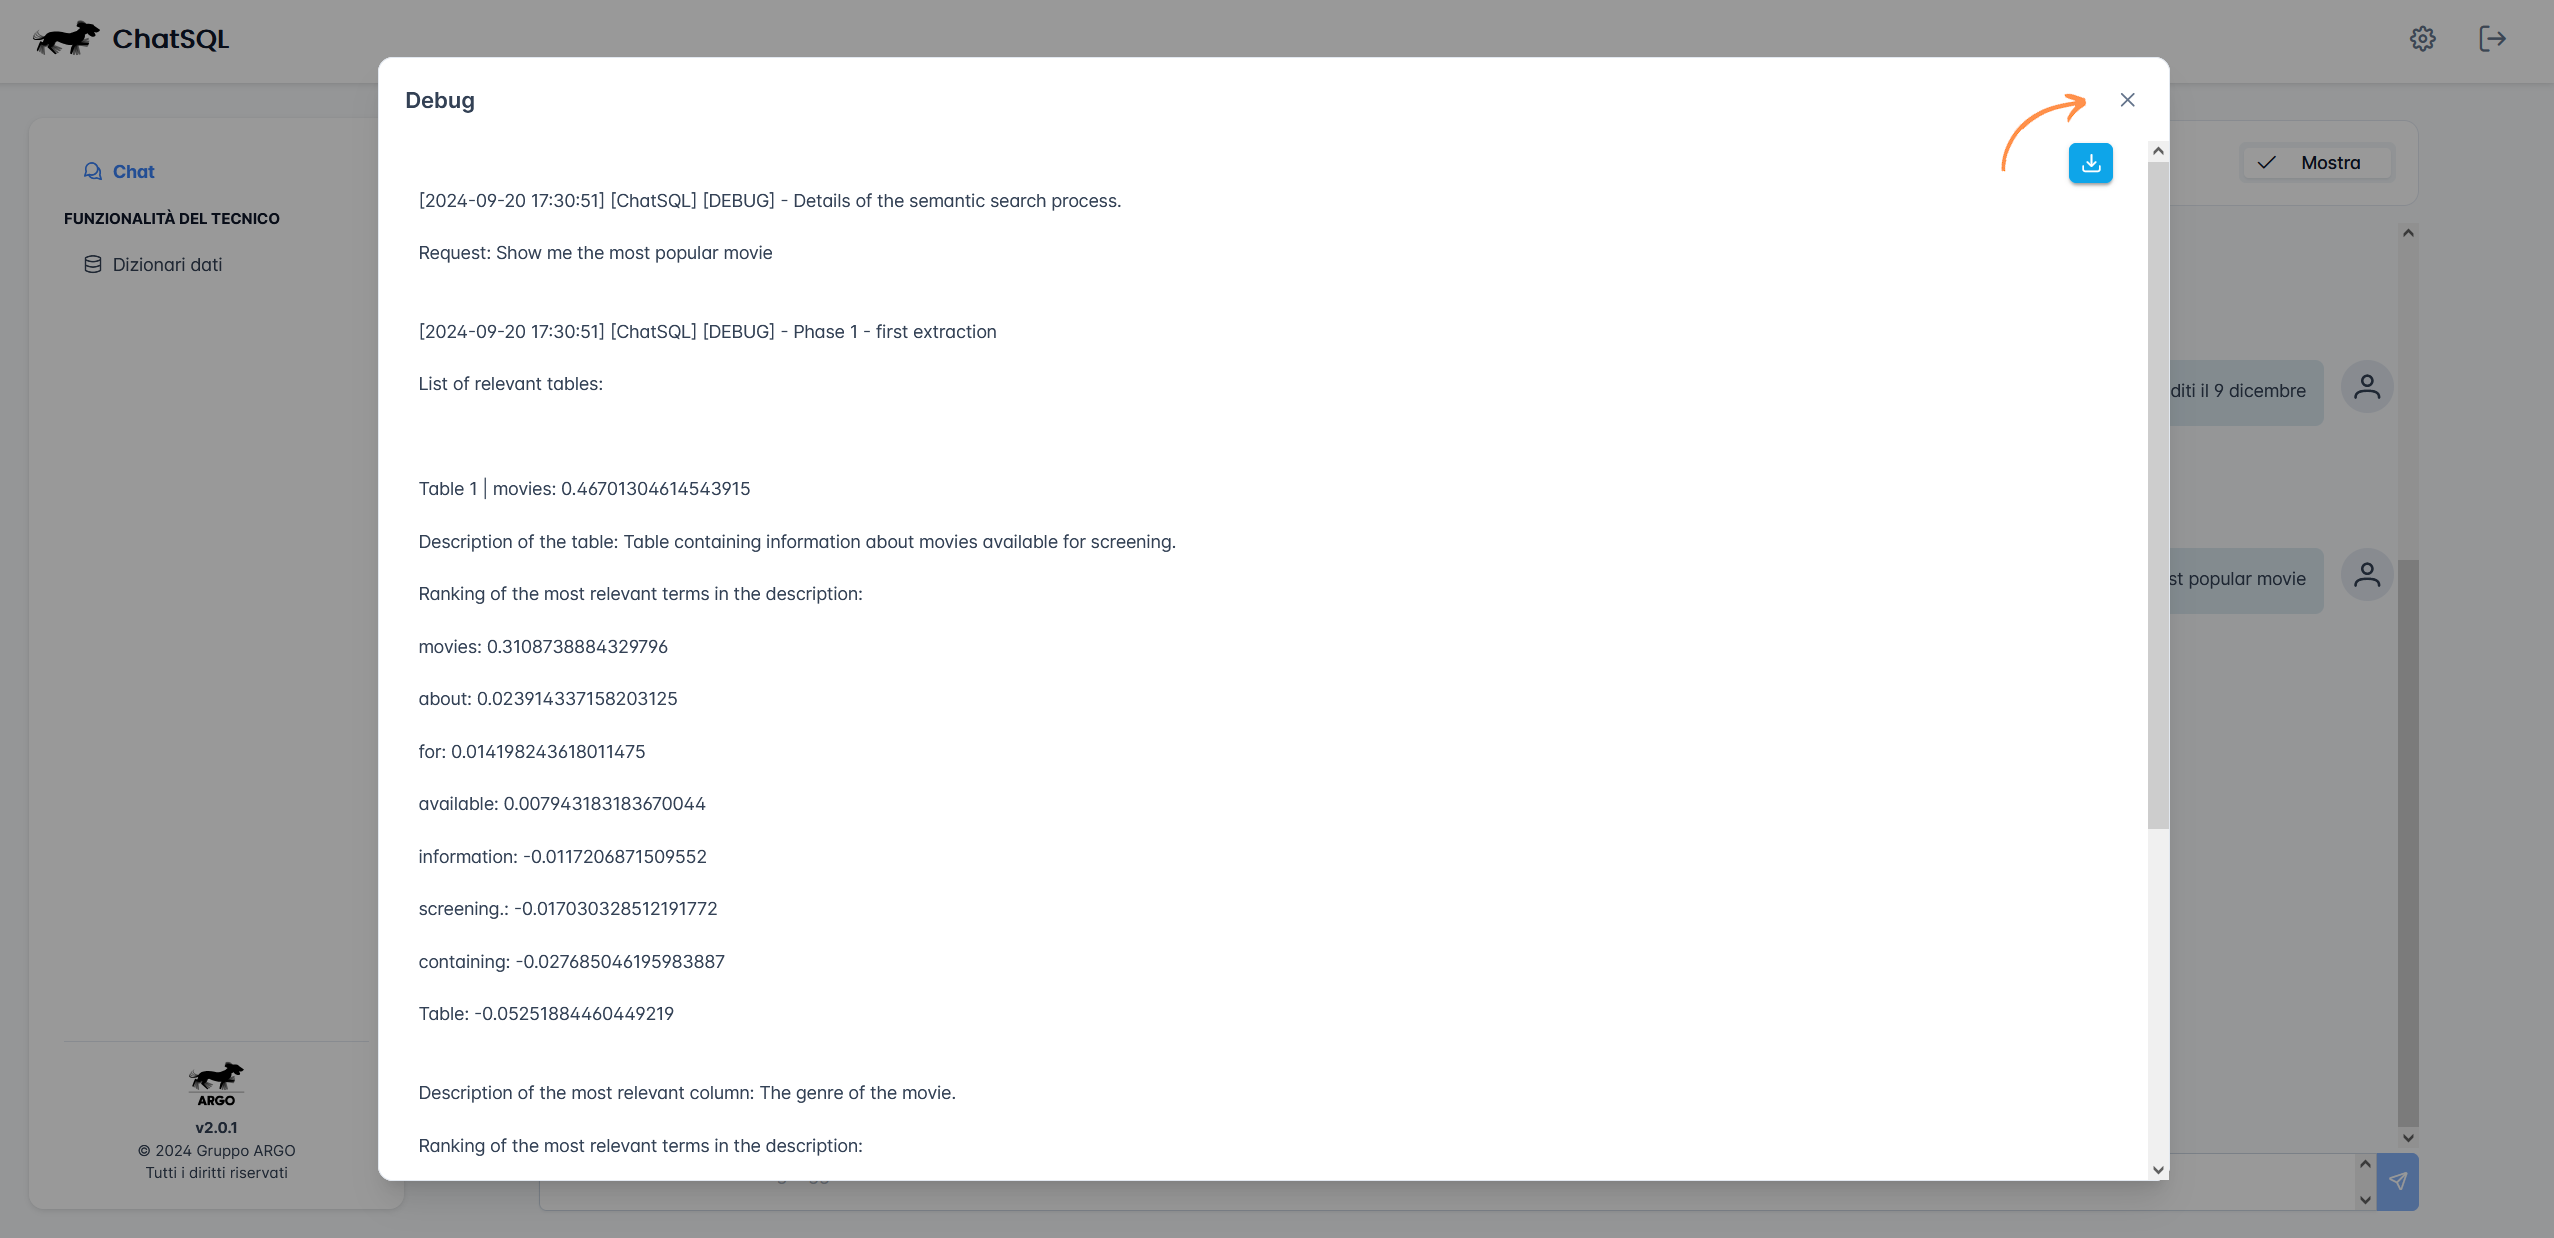
\includegraphics[width=\textwidth]{assets/tasto_close_debug.png}
  \caption{Icona chiusura messaggio di debug}
\end{figure}

\subsubsubsection{Download del messaggio di debug}

\par Il messaggio di debug può essere scaricato in formato \textit{txt}, in modo da conservarlo in locale e utilizzarlo per migliorare il \glossario{dizionario dati} o per produrre analisi a posteriori.
\begin{figure}[H]
  \centering
  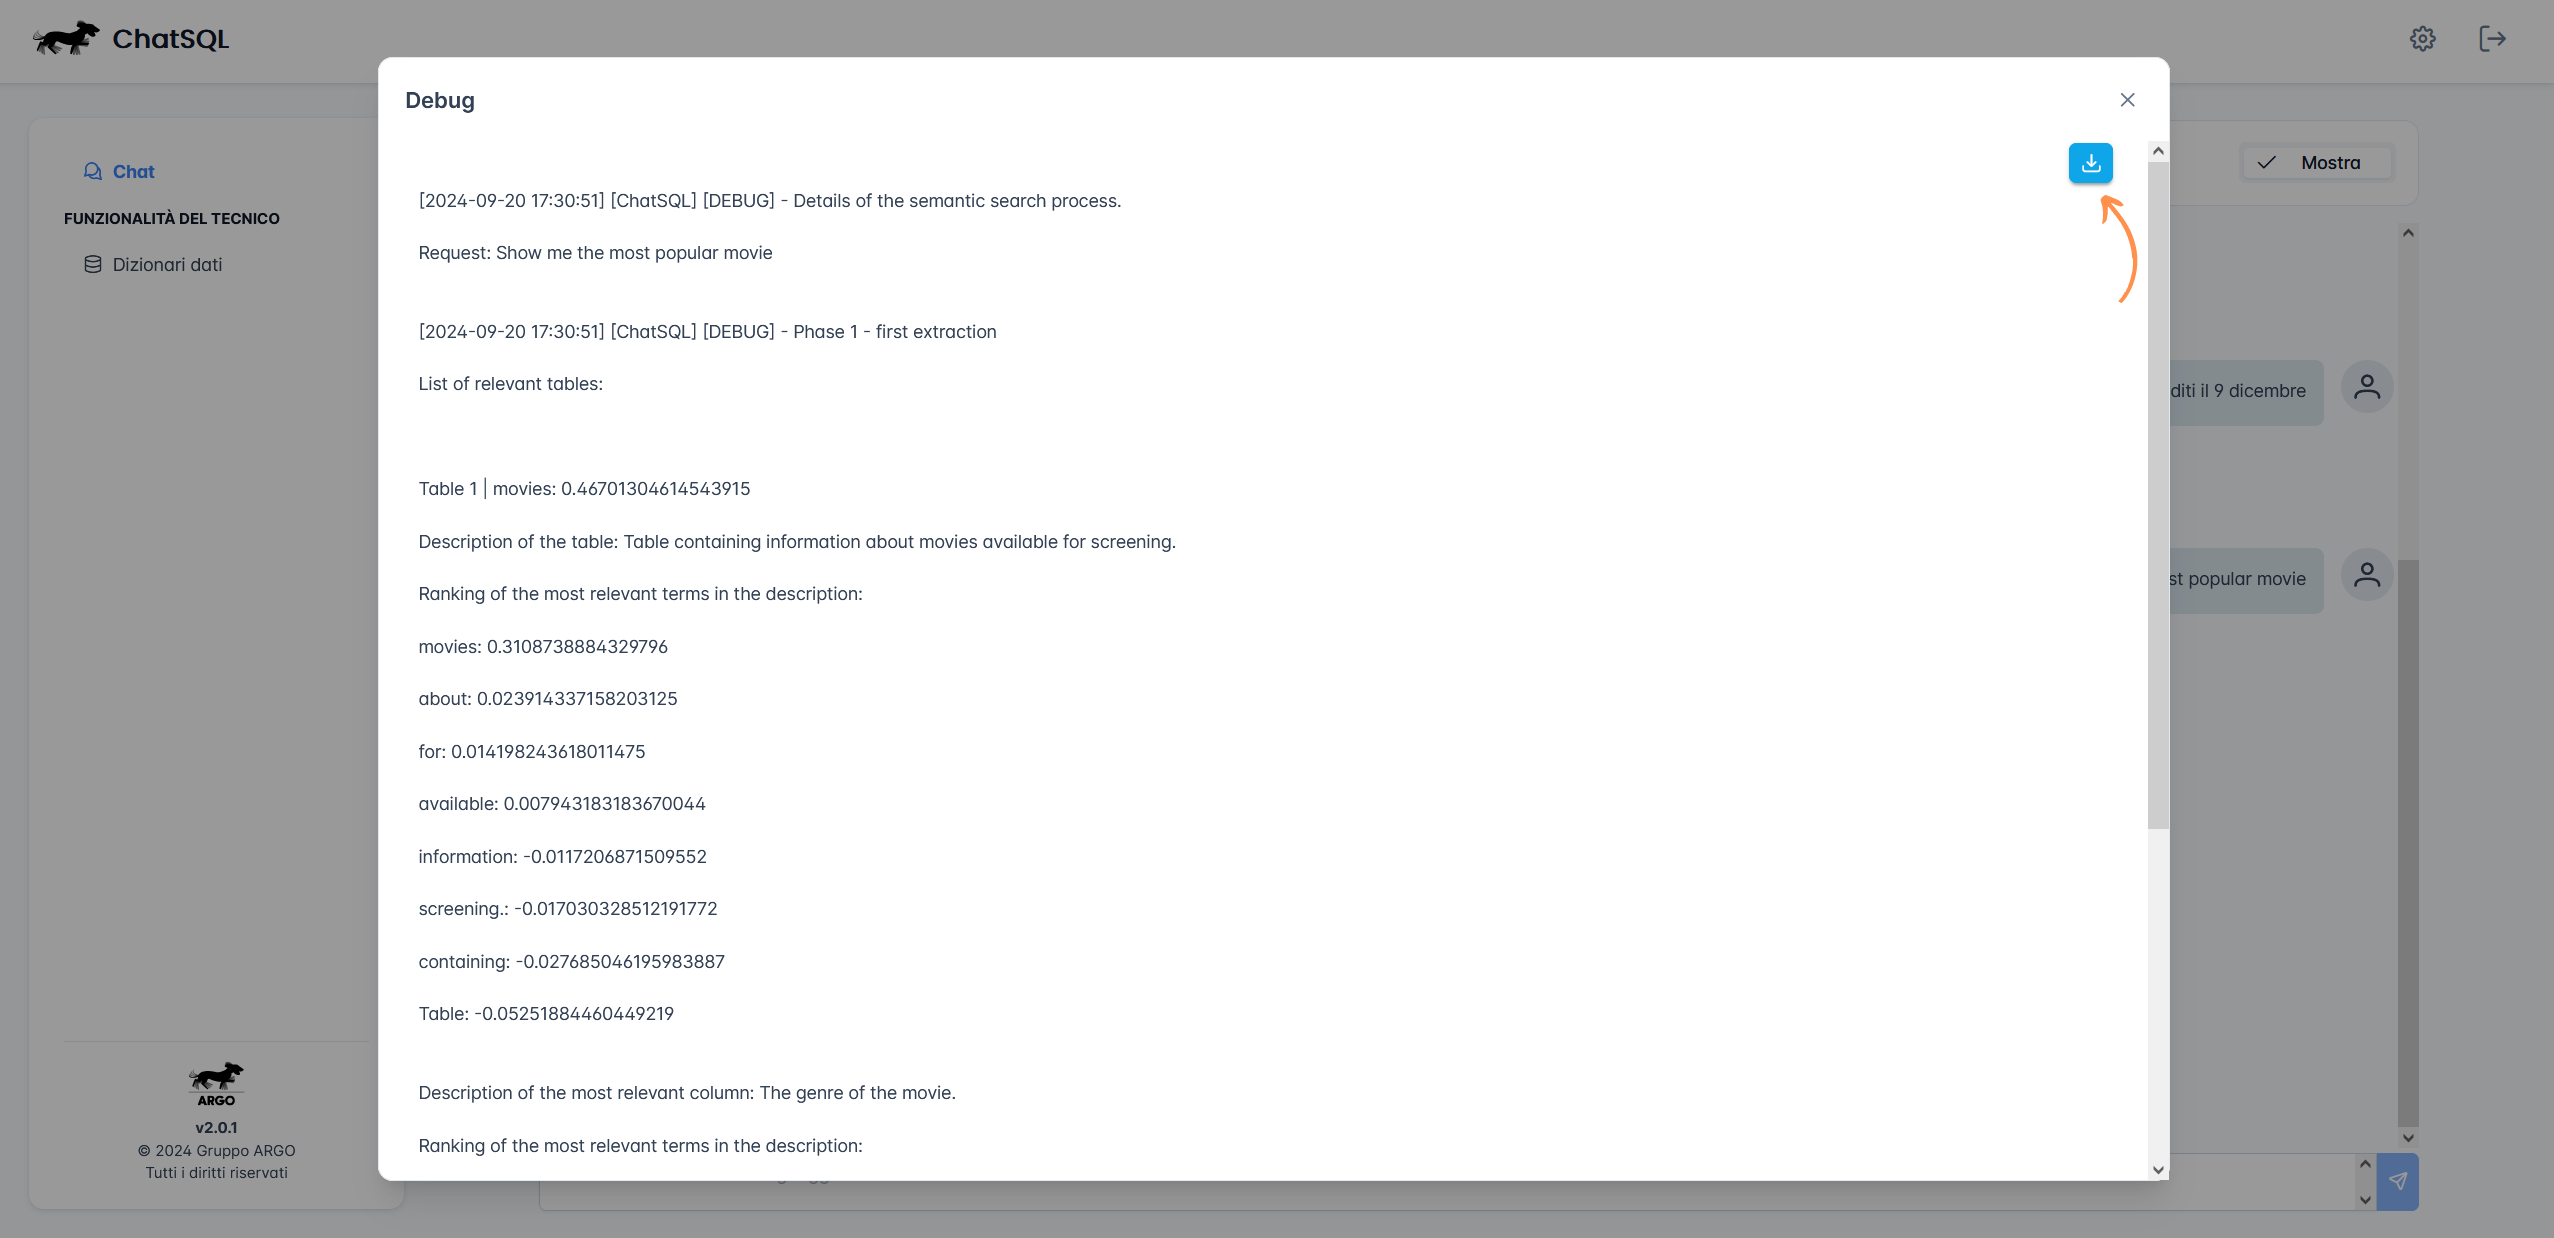
\includegraphics[width=\textwidth]{assets/tasto_dawnload_debug.png}
  \caption{Download del messaggio di debug}
\end{figure}






\subsection{Workflow}
\par Nell'utilizzo di ChatSQL, il flusso più comune da seguire per ottenere una query SQL è:
\begin{enumerate}
  \item Accedere alla pagina Chat selezionandola dal menu di navigazione principale;
  \item Selezionare il \glossario{dizionario dati} desiderato;
  \item Selezionare il \glossario{DBMS} desiderato;
  \item Selezionare la lingua desiderata;
  \item Inserire una richiesta in linguaggio naturale e attendere la generazione del \glossario{prompt};
  \item Copiare il prompt generato cliccando sull'apposito pulsante in alto a destra all'interno del messaggio fornito dal ChatBOT;
  \item Incollare il prompt in un modello \glossario{LLM} a scelta (come ChatGPT) e attendere la generazione della query SQL.
\end{enumerate}

\vspace{\baselineskip}
\par Di seguito è riportata una figura che illustra nel dettaglio il flusso da seguire per ottenere una query SQL da utilizzare per interrogare database reali.

\begin{figure}[H]
  \fbox{
  \begin{tabular}{cc}
    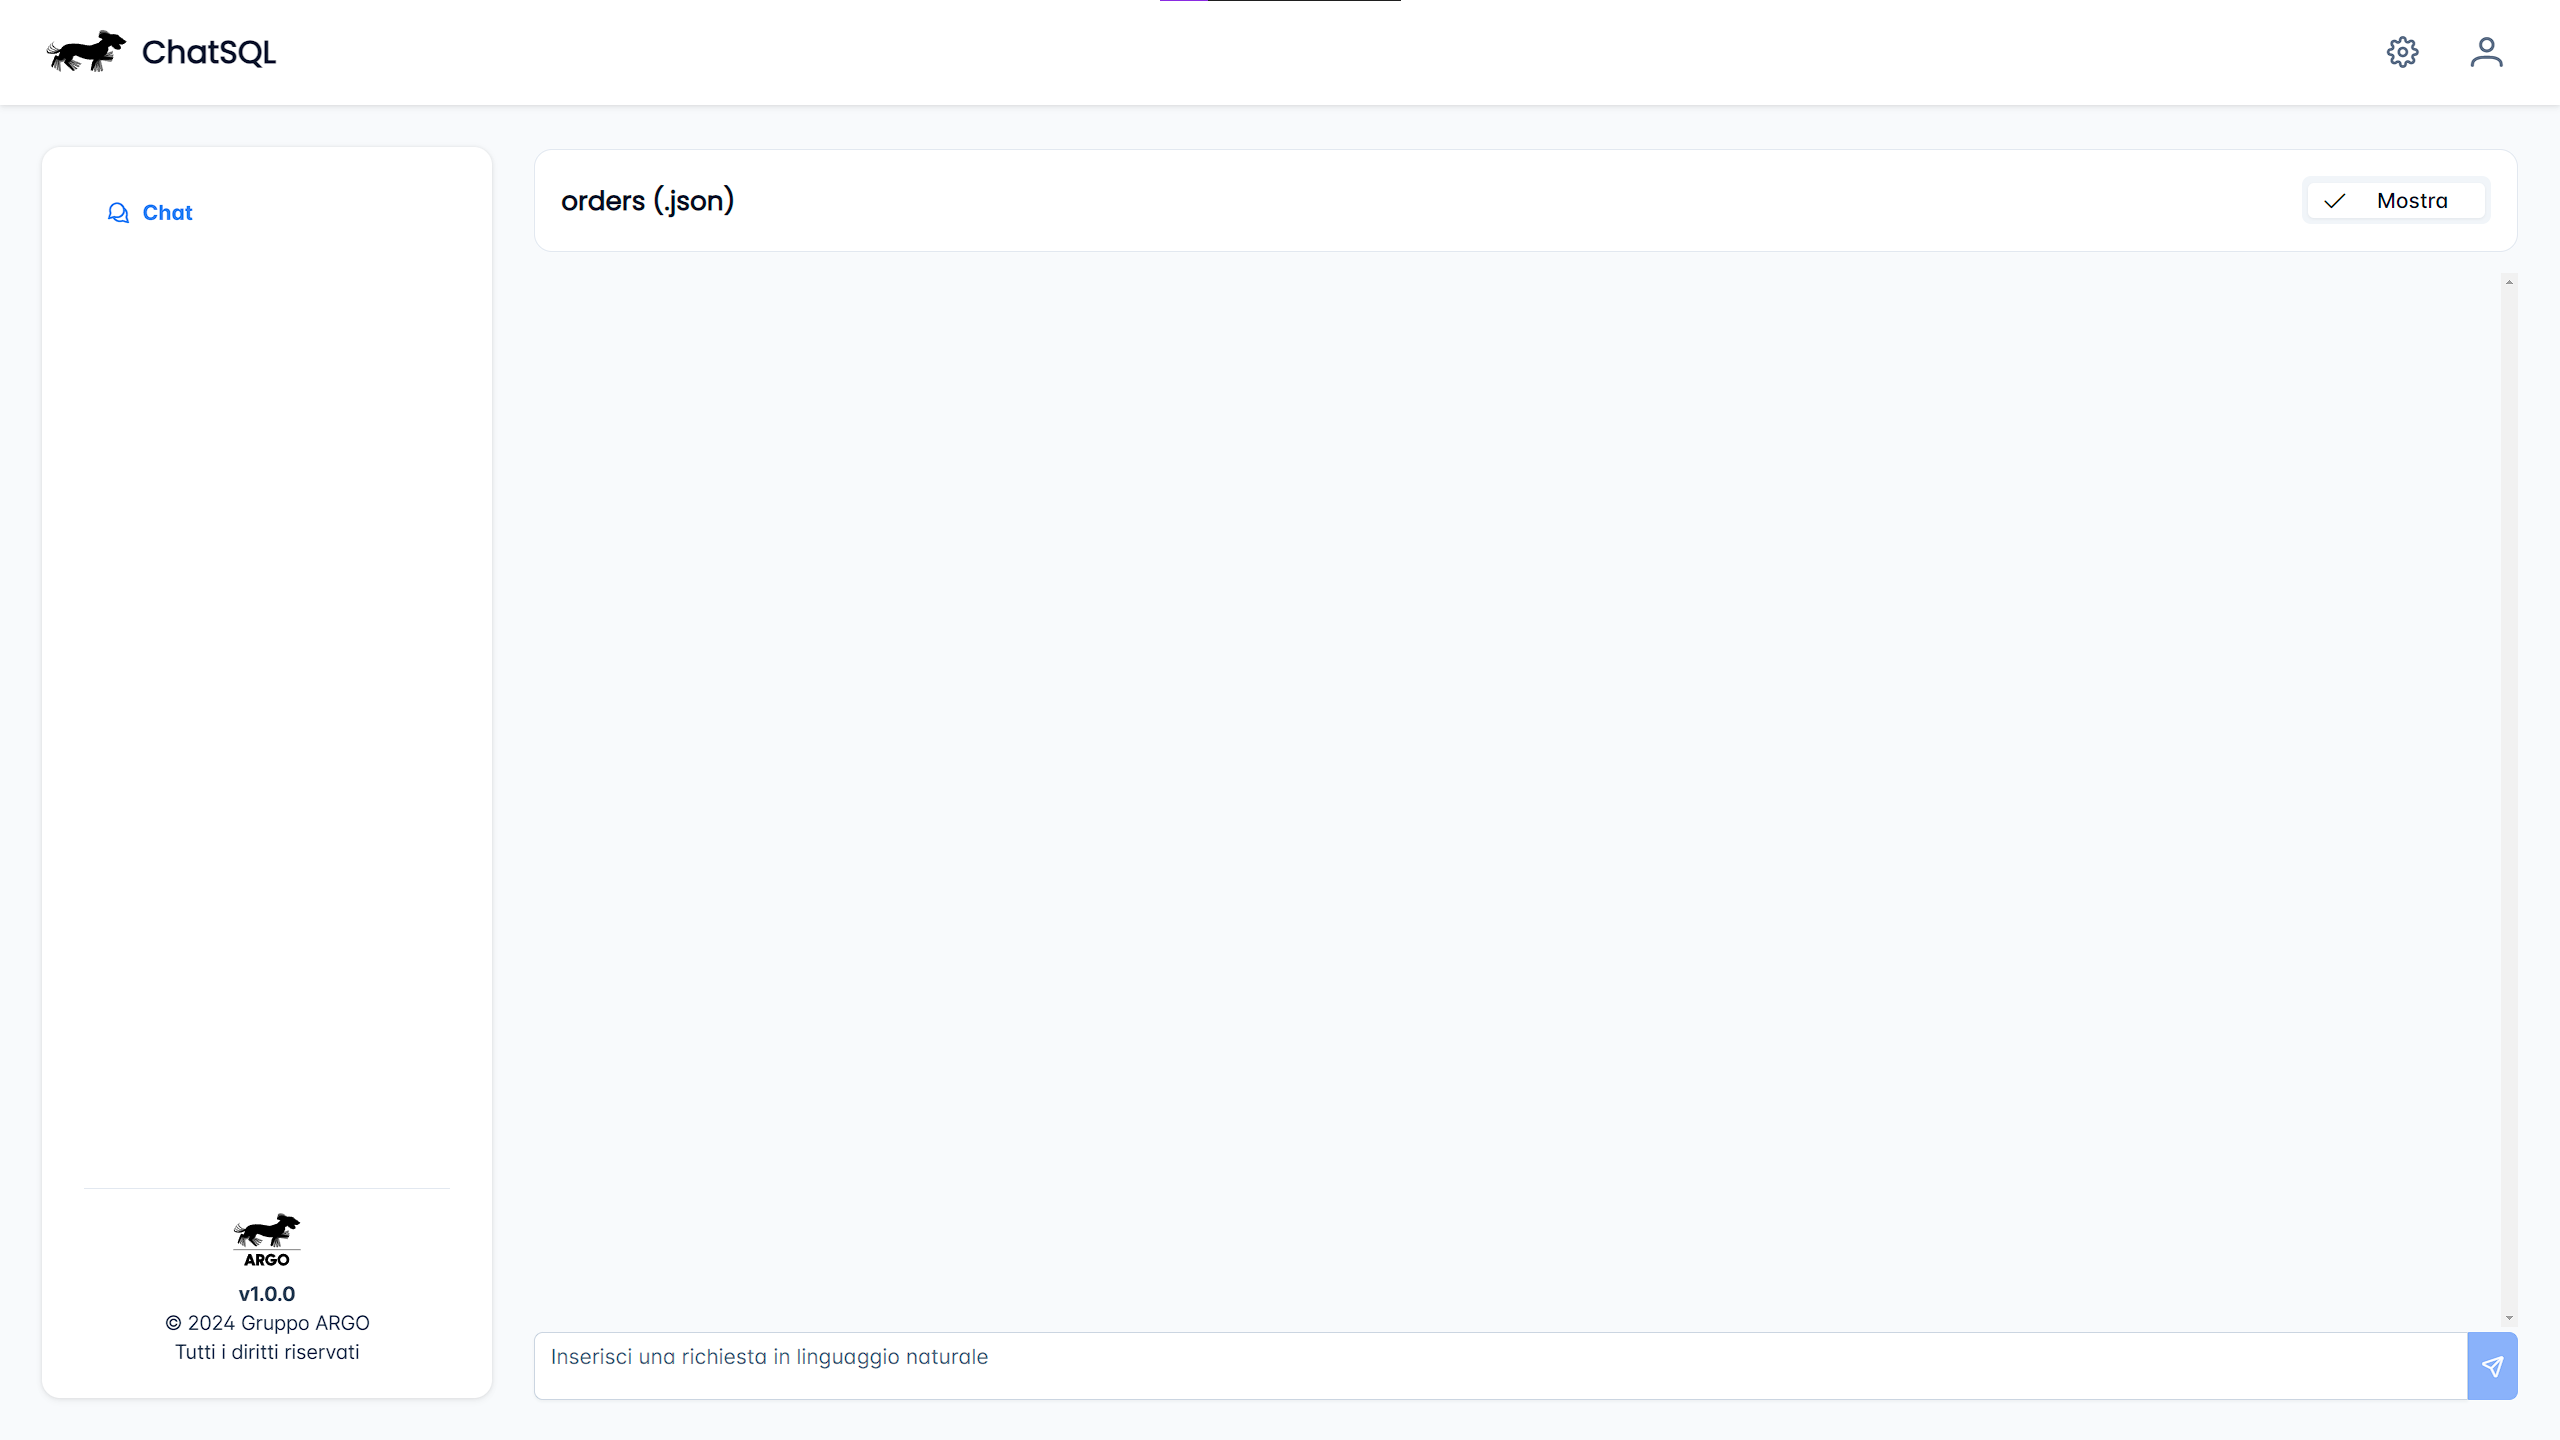
\includegraphics[width=65mm]{assets/workflow_1.png} &   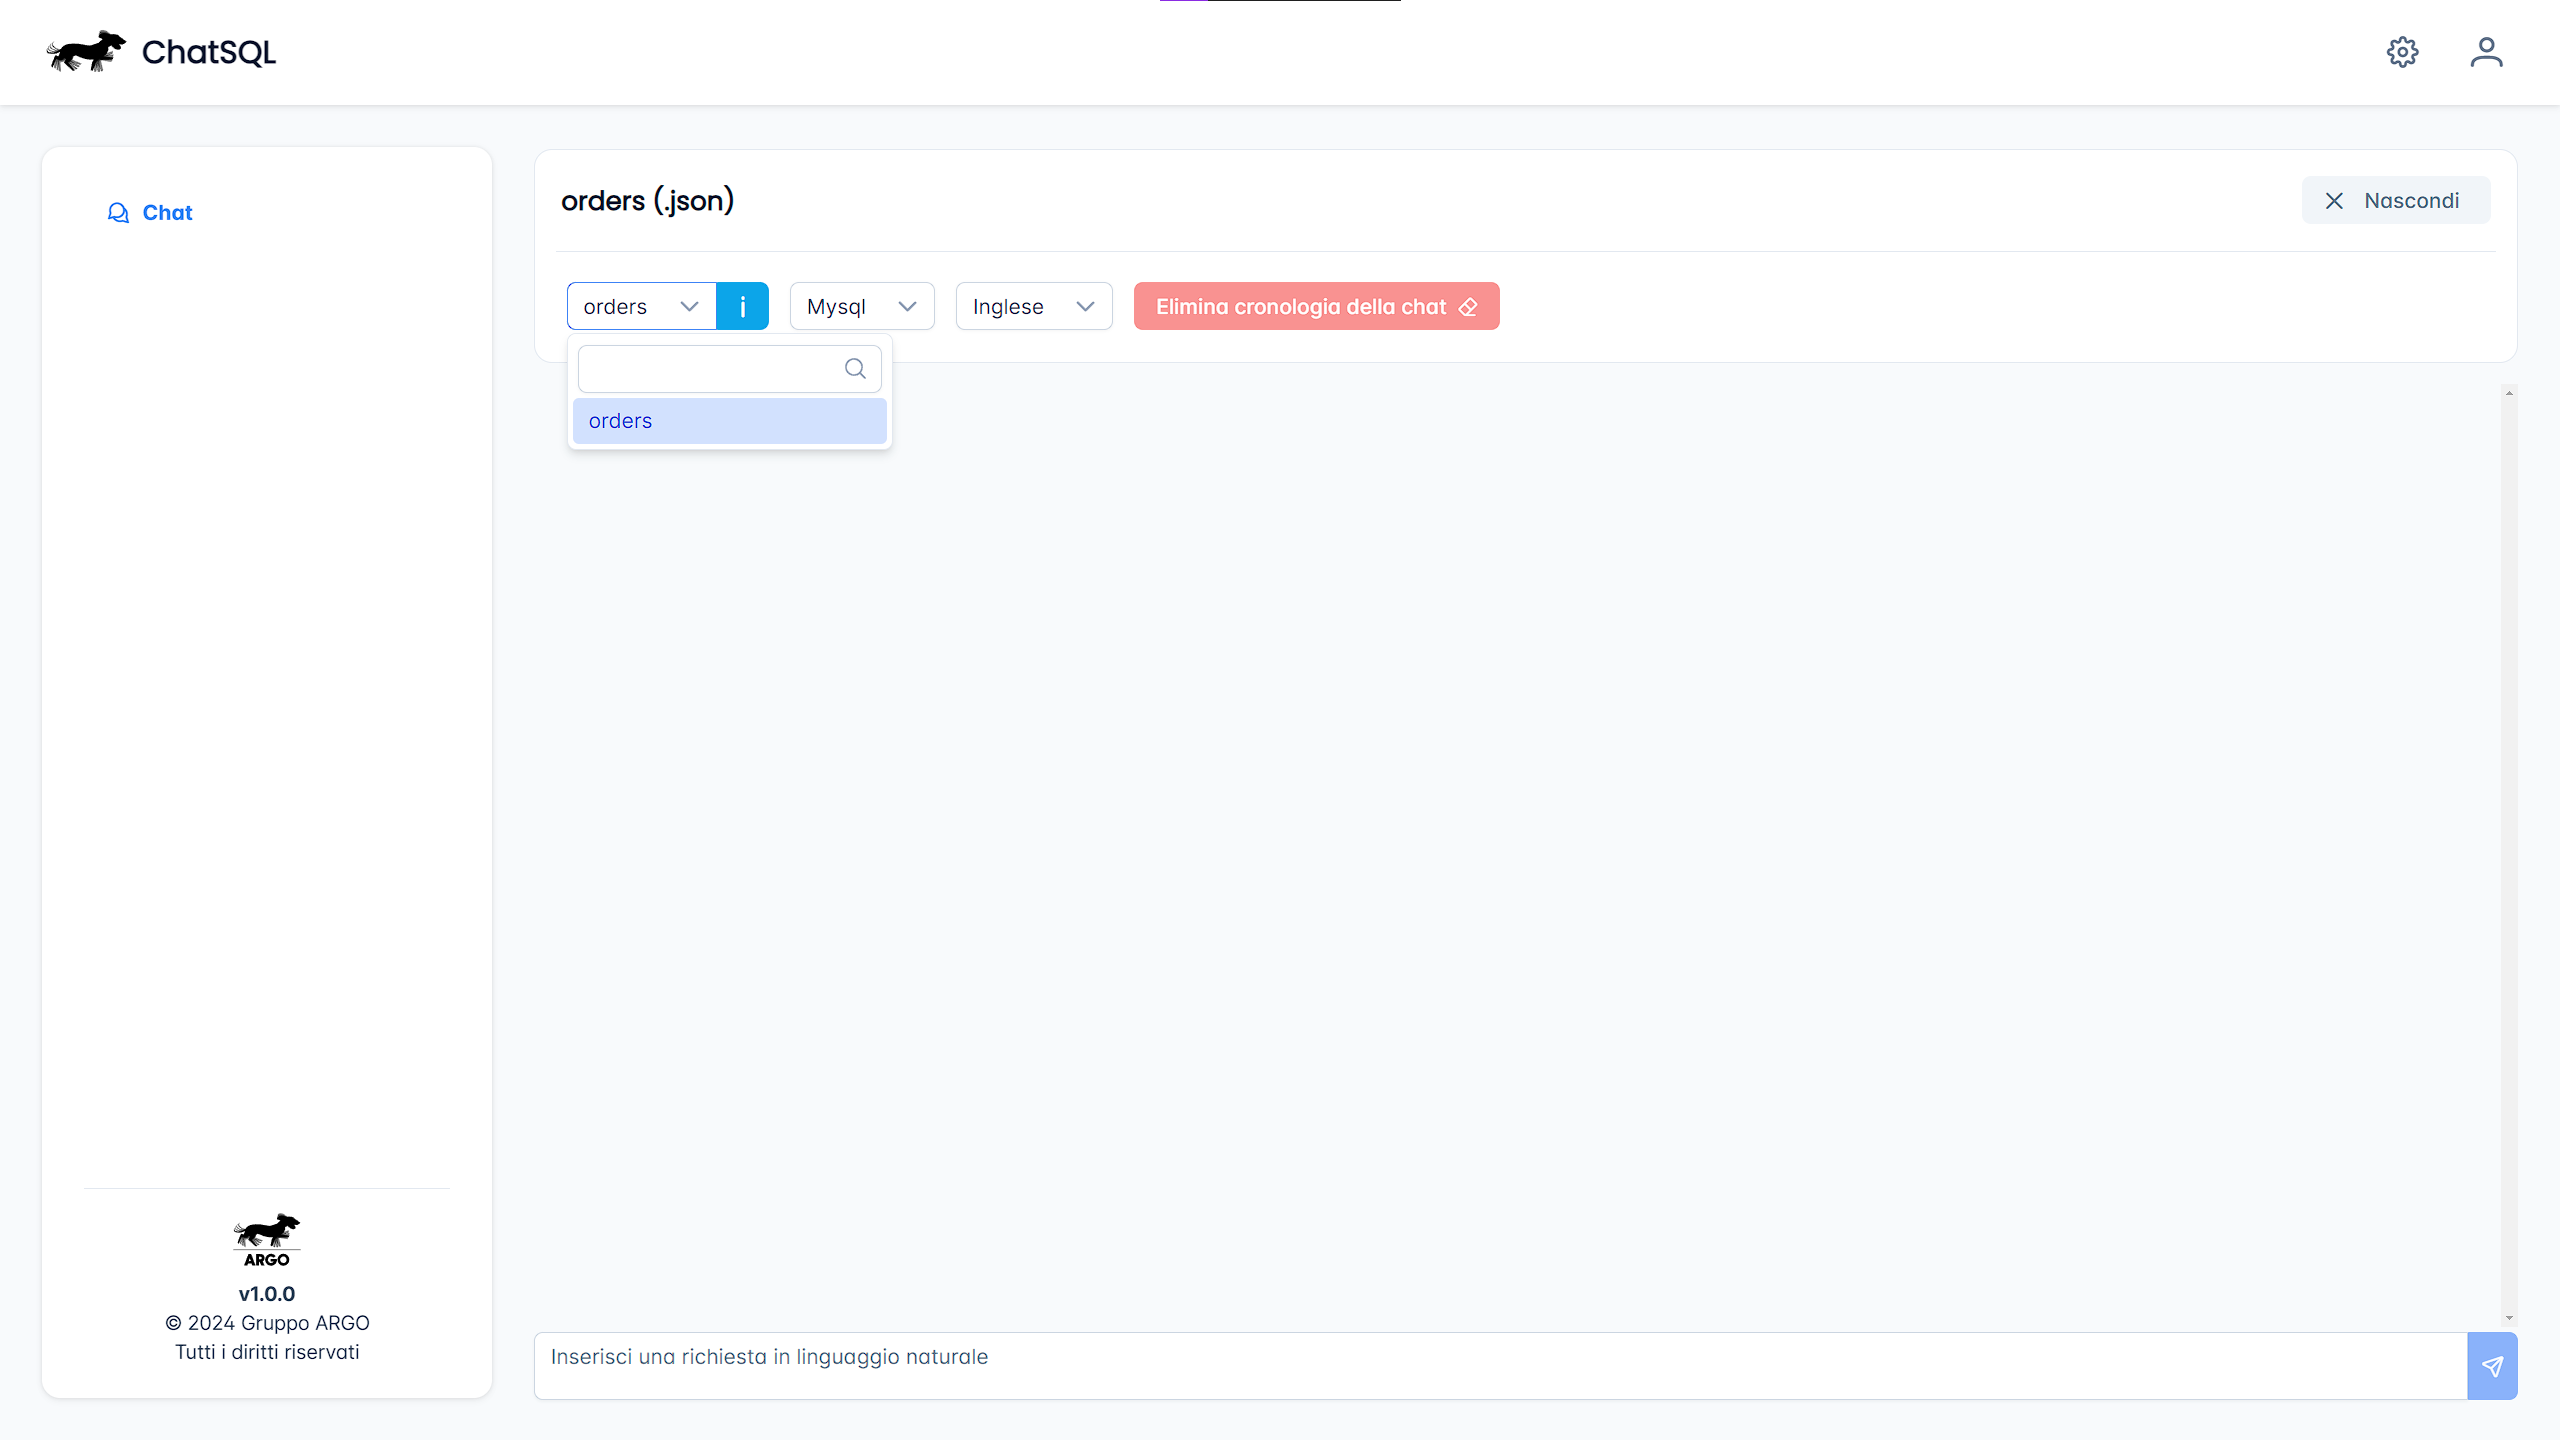
\includegraphics[width=65mm]{assets/workflow_2.png} \\
    1 & 2 \\[6pt]
     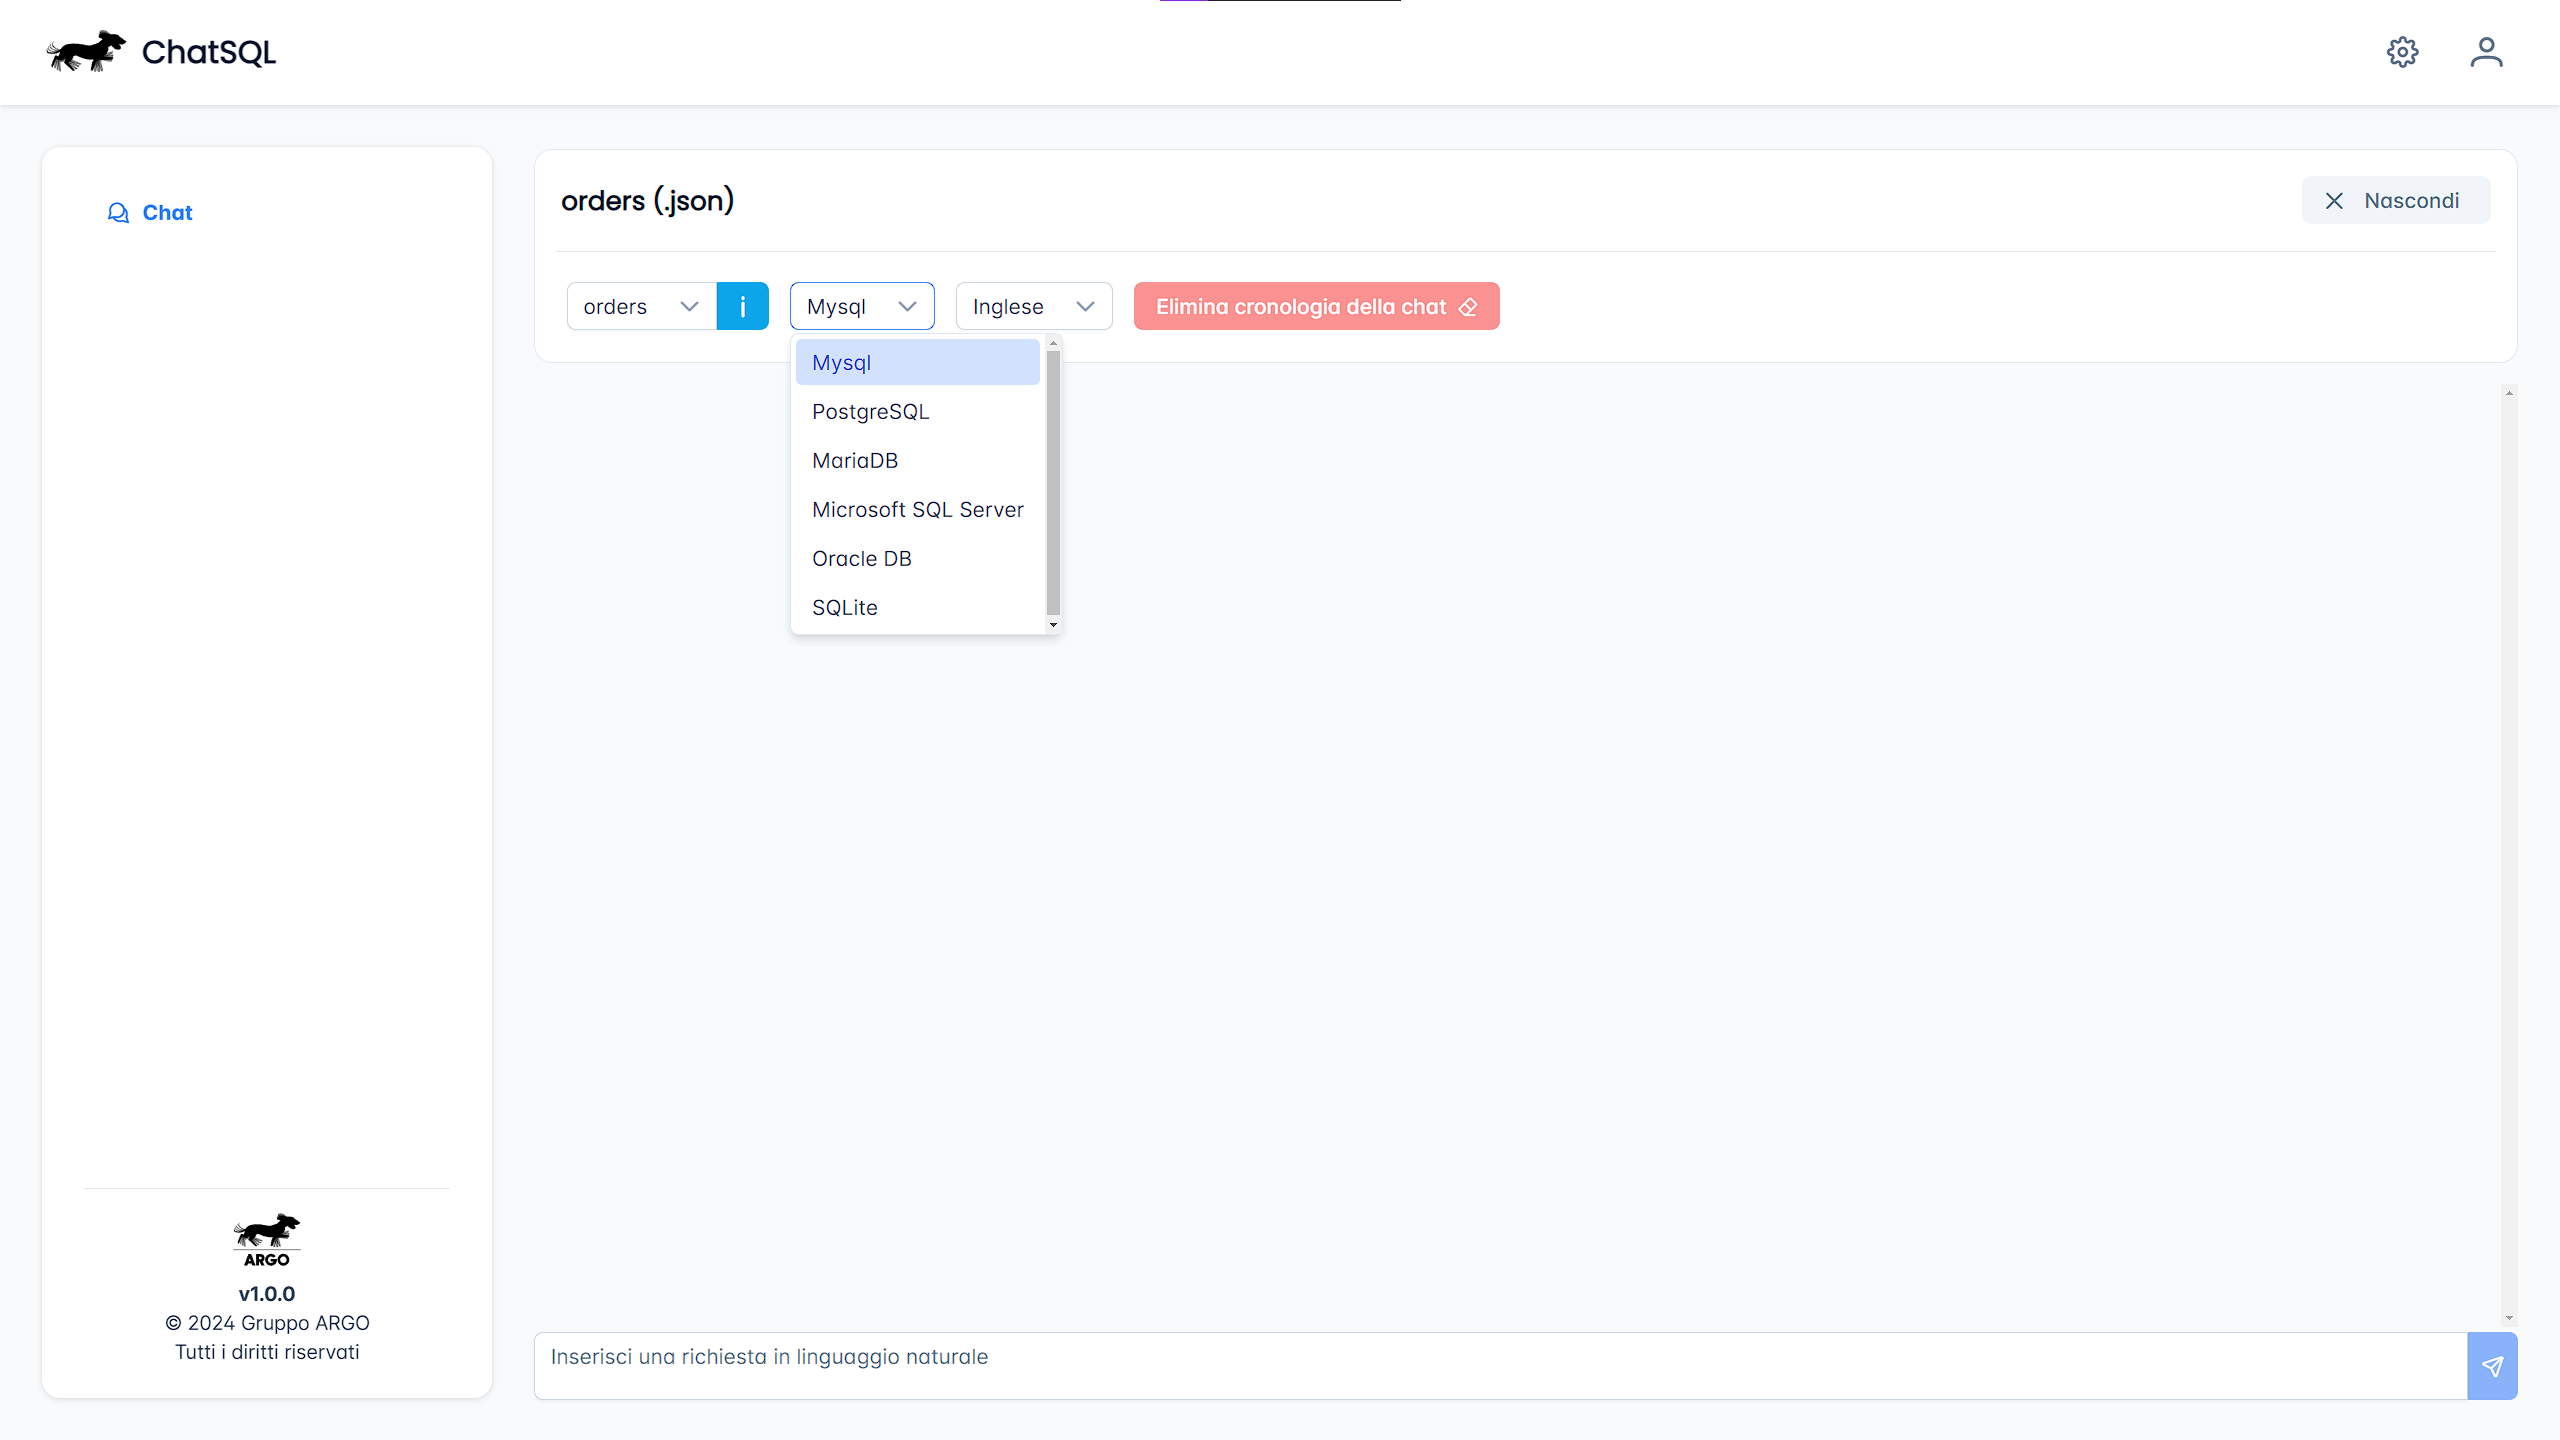
\includegraphics[width=65mm]{assets/workflow_3.png} &   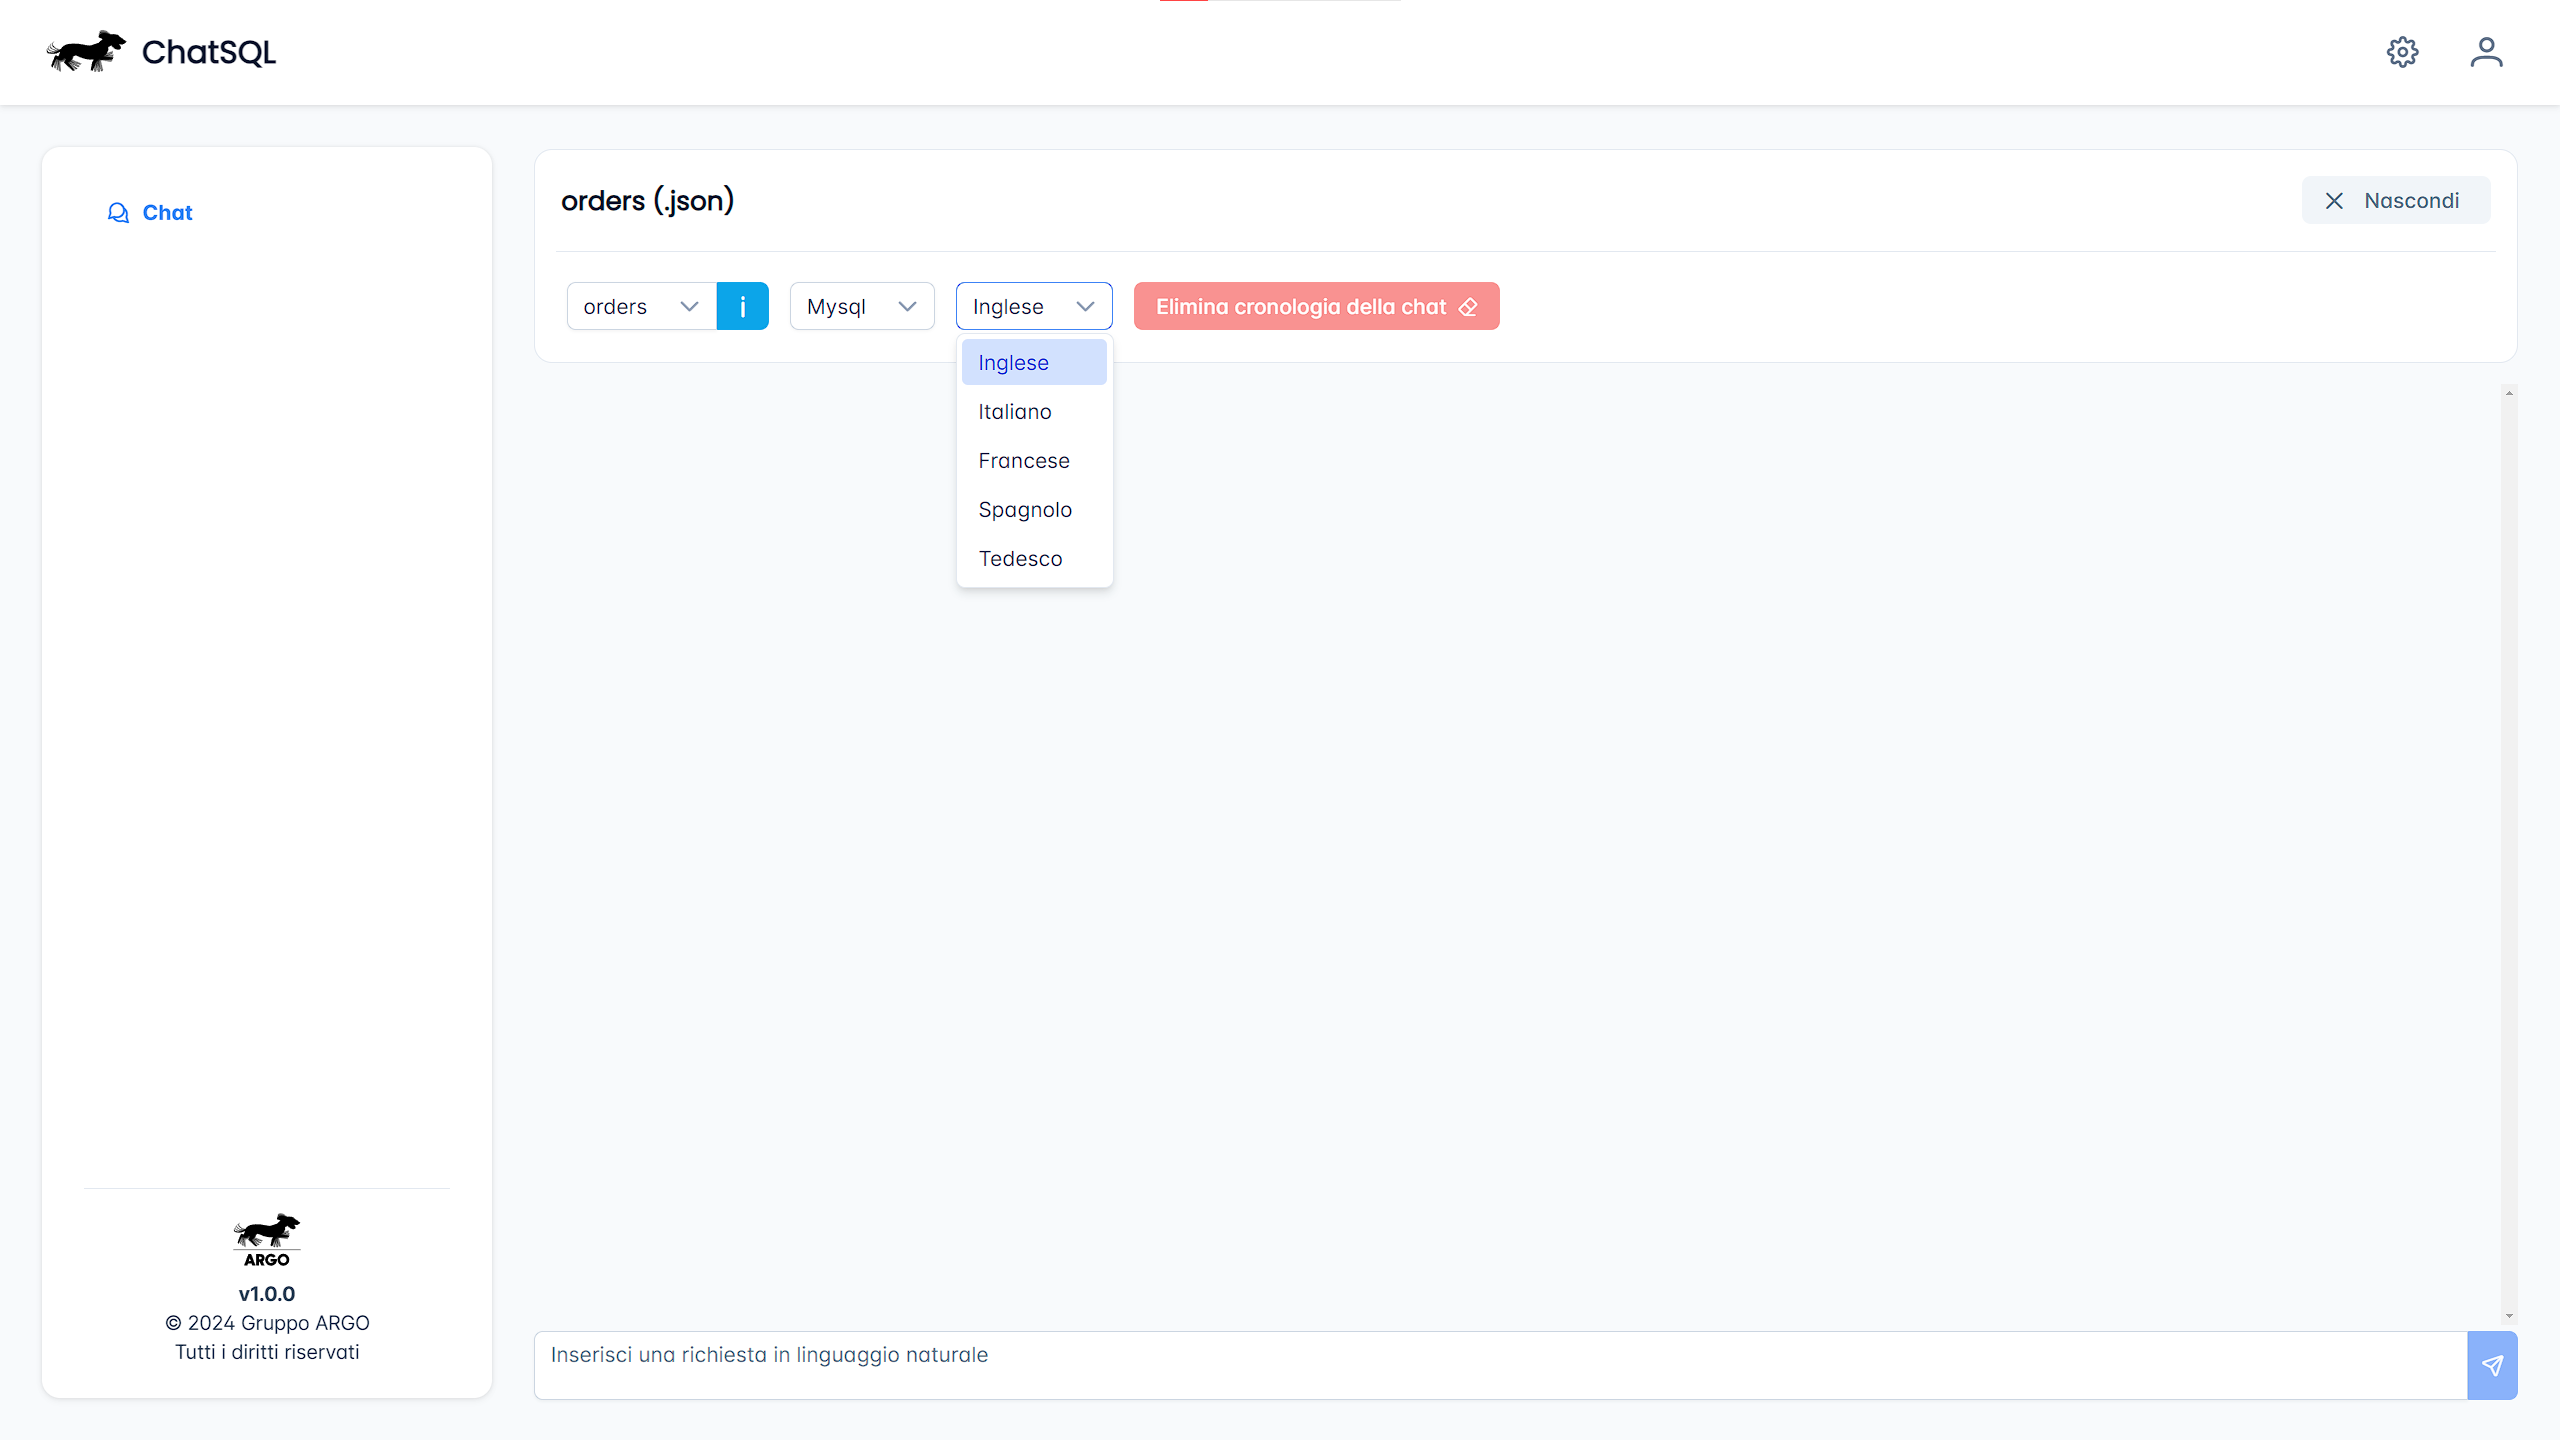
\includegraphics[width=65mm]{assets/workflow_4.png} \\
    3 & 4 \\[6pt]
   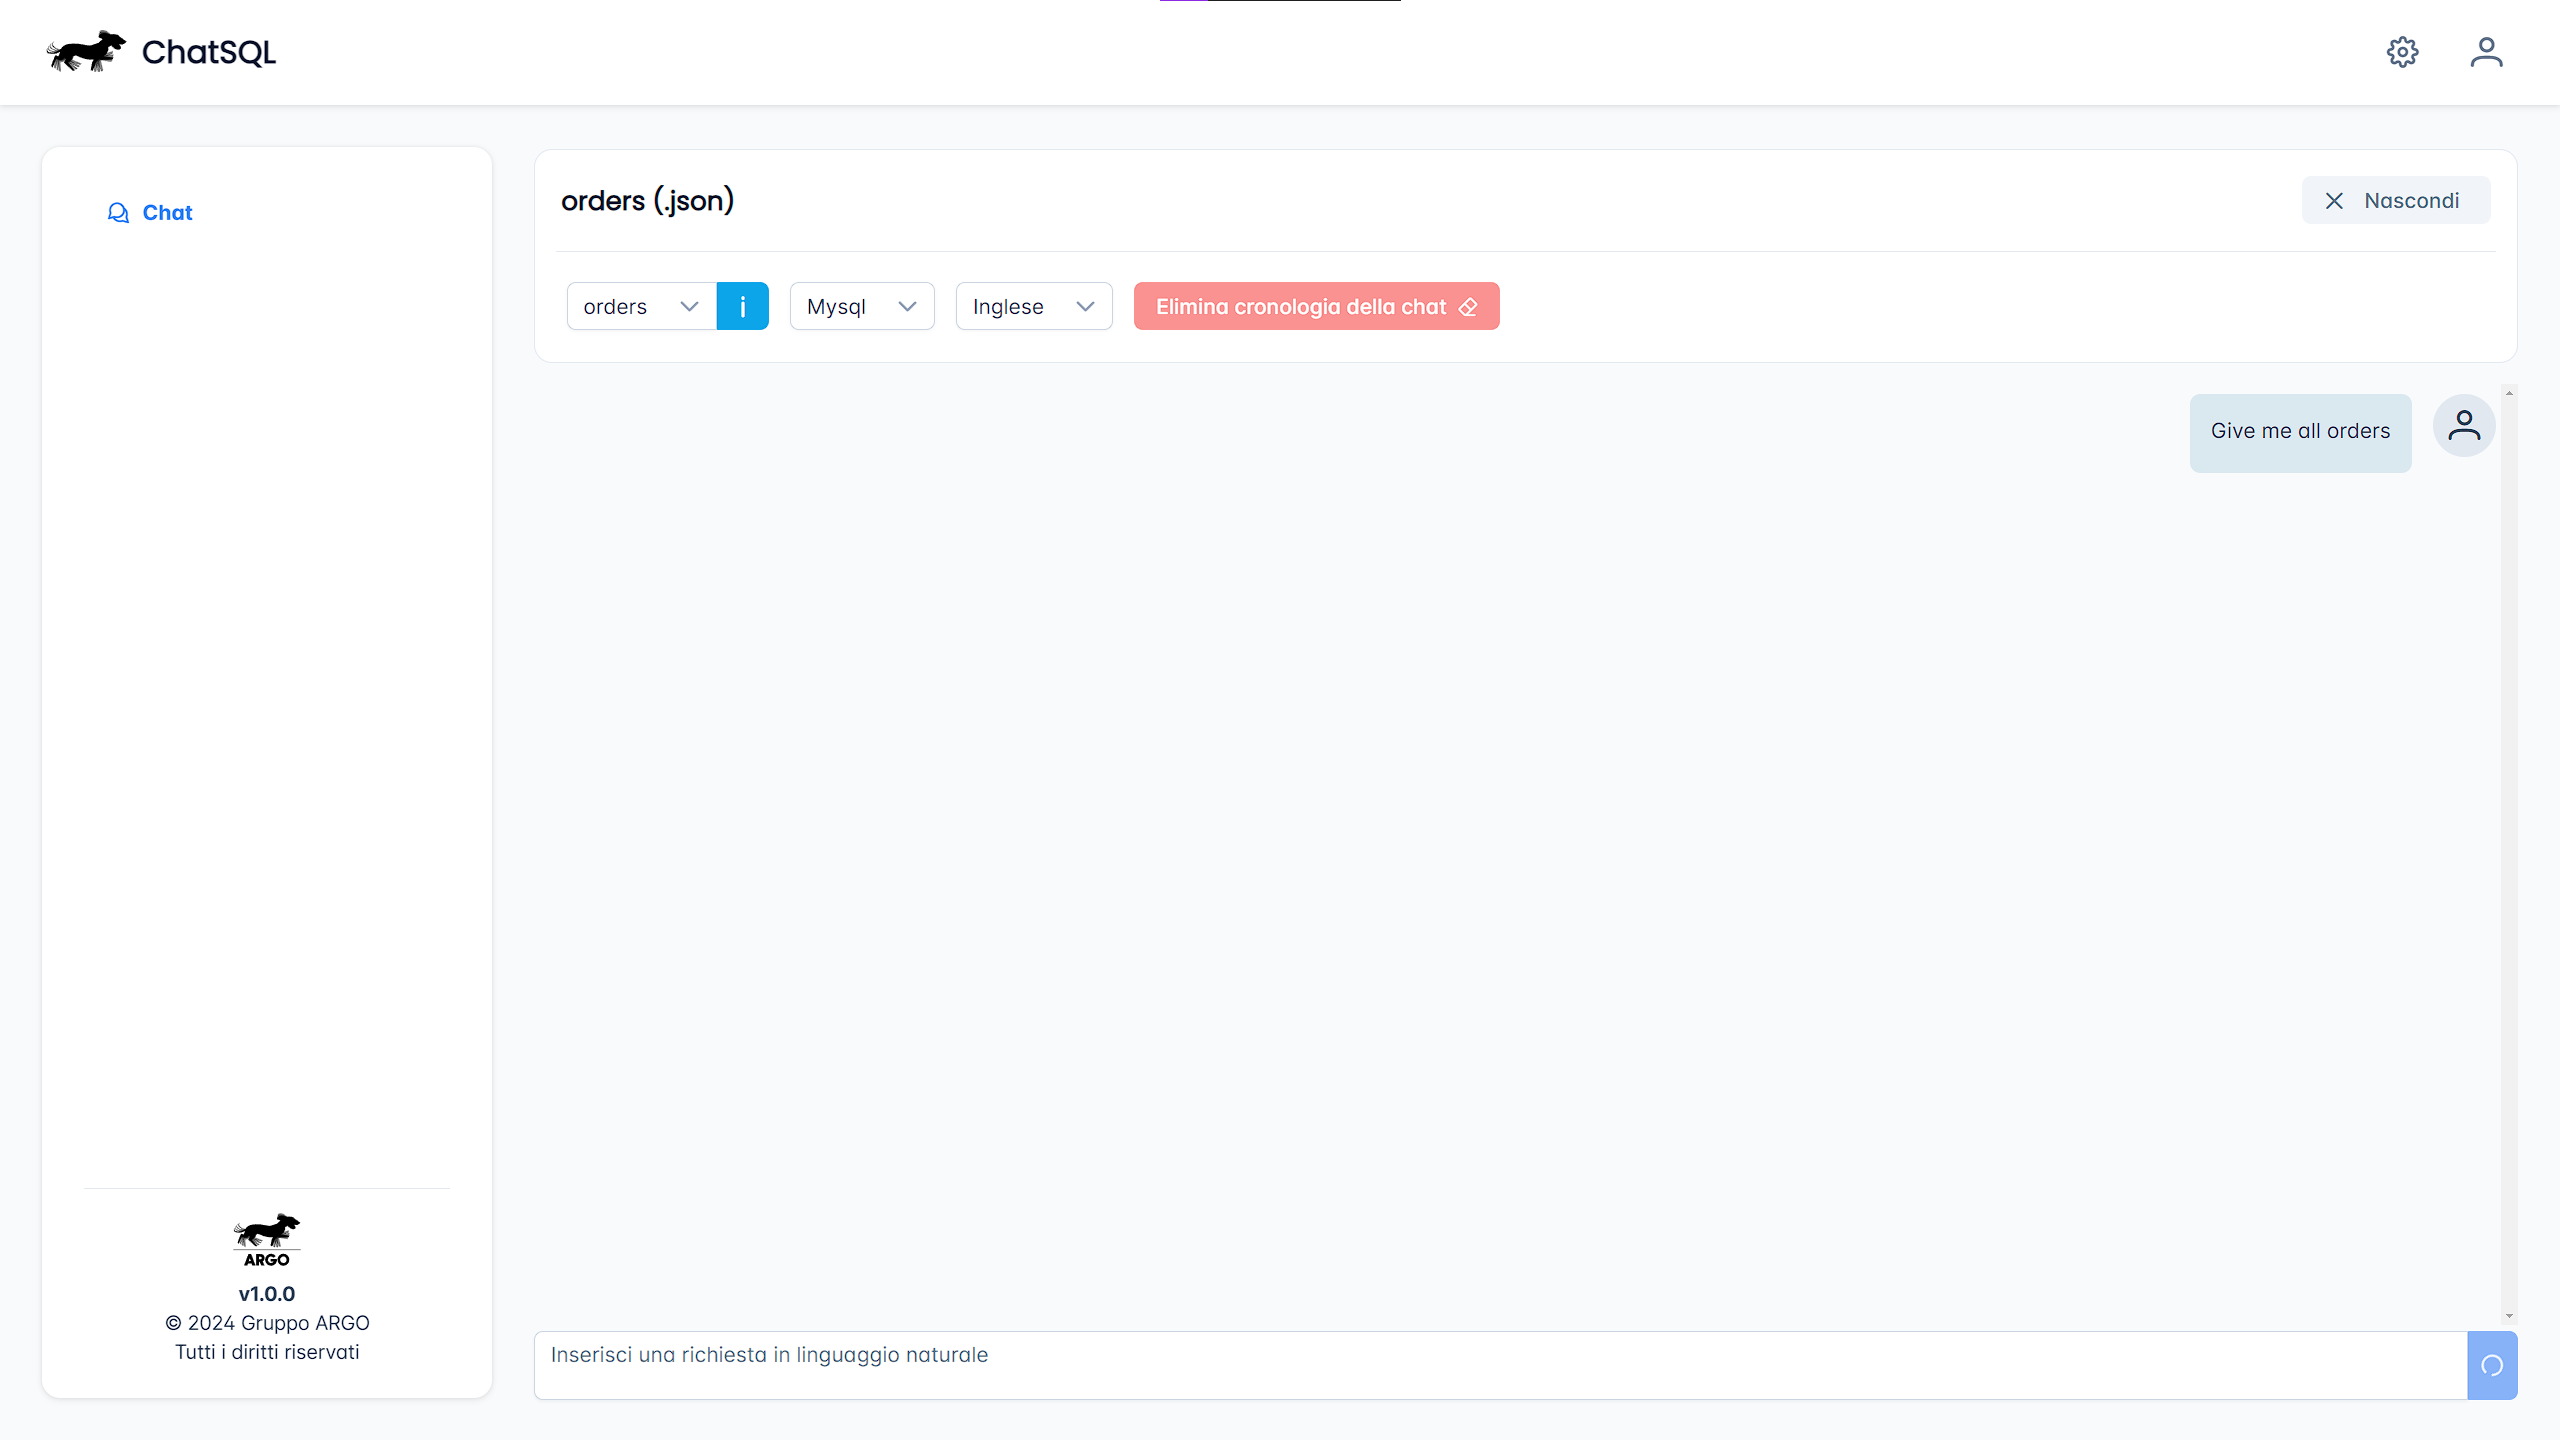
\includegraphics[width=65mm]{assets/workflow_5.png} &   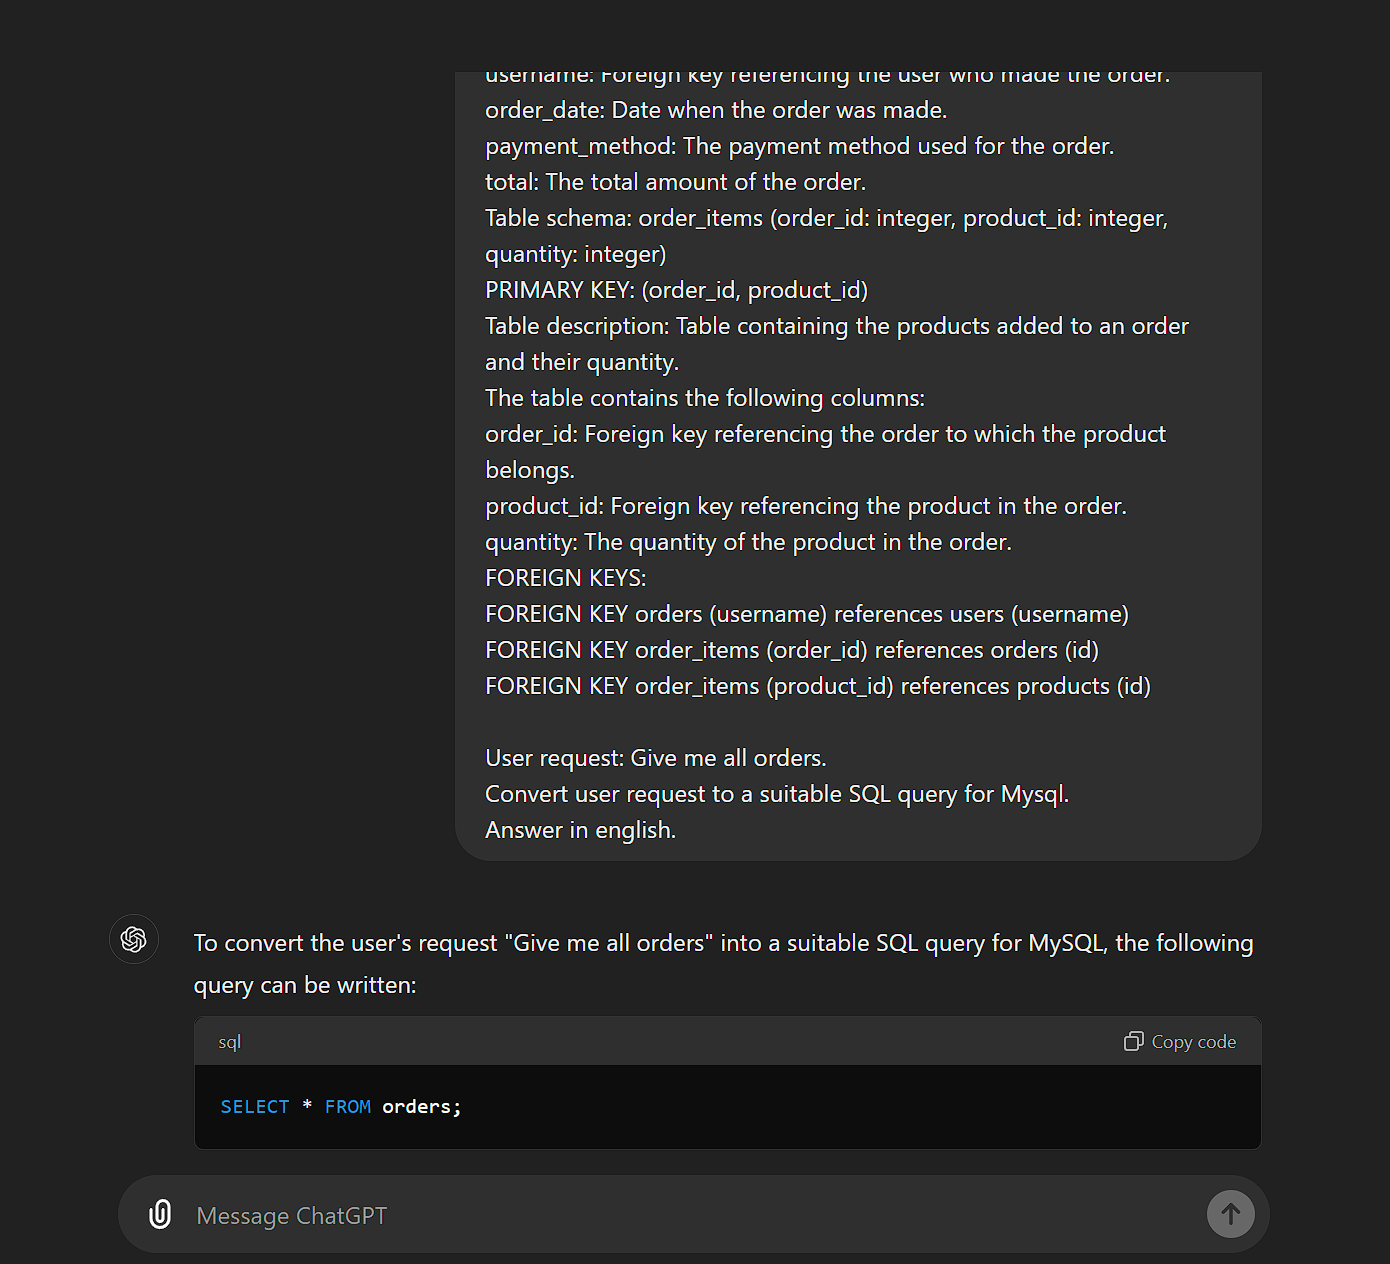
\includegraphics[width=65mm]{assets/workflow_6.png} \\
    5 & 6 \\[6pt]
    \multicolumn{2}{c}{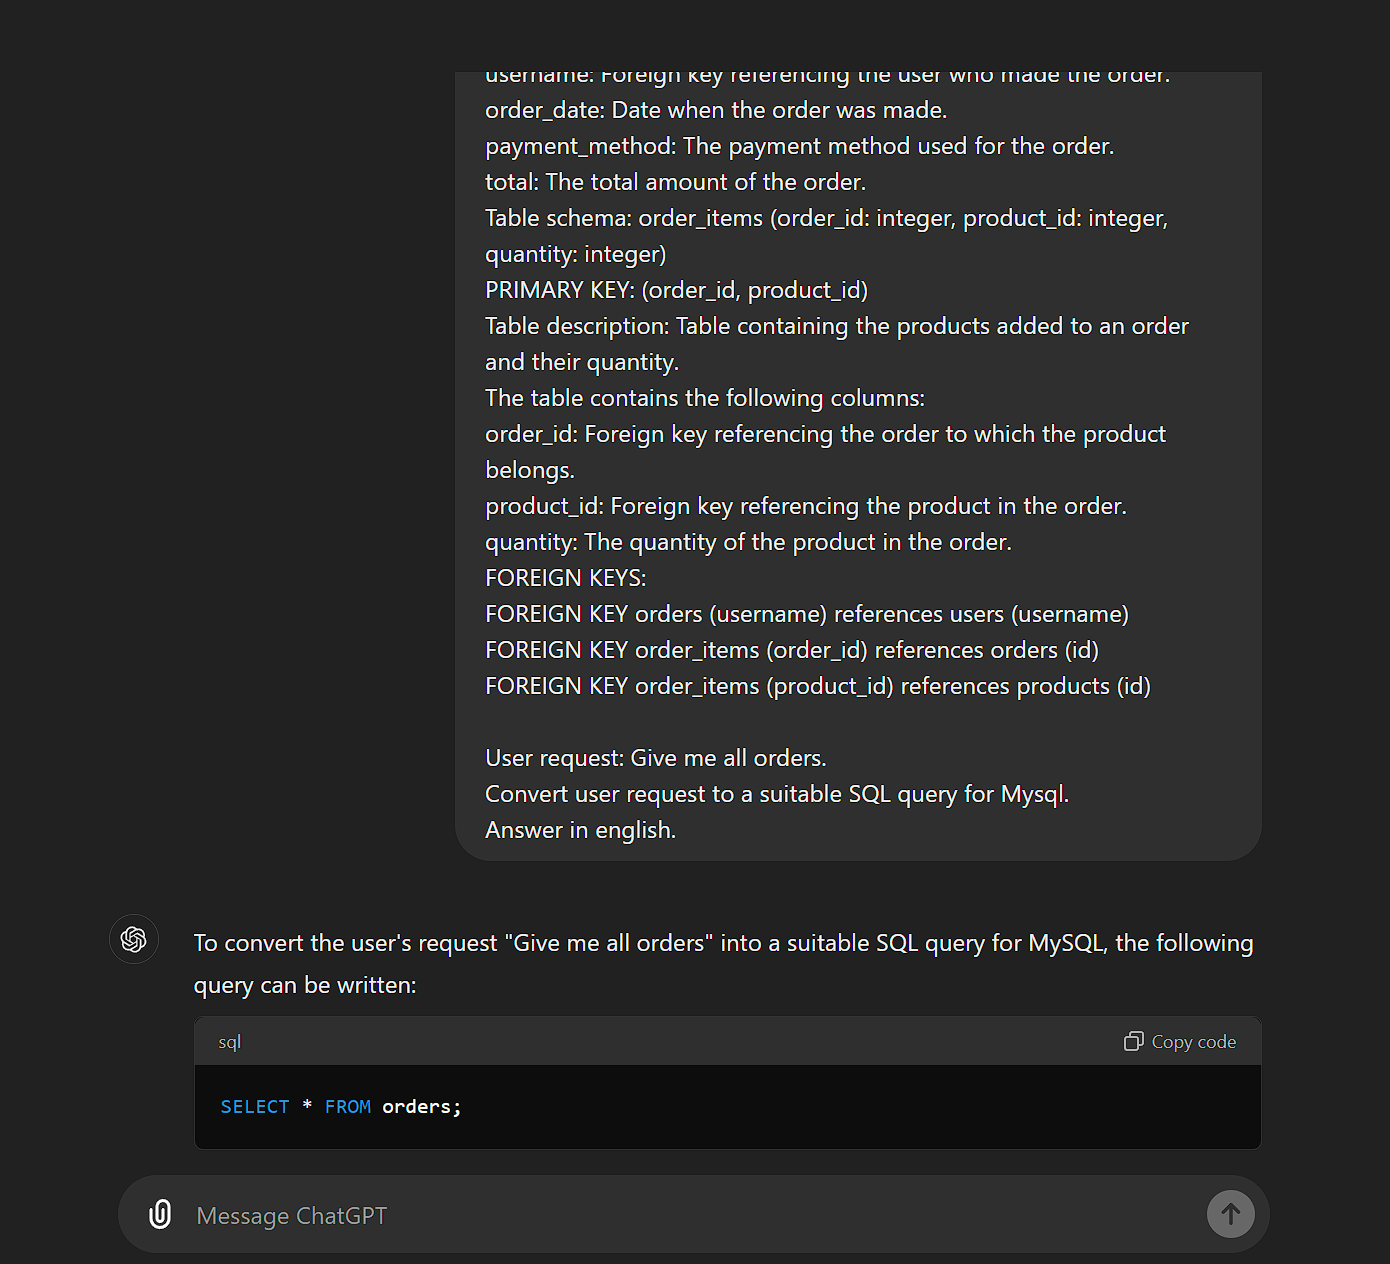
\includegraphics[width=65mm]{assets/workflow_7.png}}\\
    \multicolumn{2}{c}{7}
  \end{tabular}}
  \caption{Workflow per ottenere una query SQL}
\end{figure}
\par L'output atteso dal modello LLM è una query SQL che soddisfa la richiesta inserita, che potrà essere eseguita su un DBMS per ottenere i risultati desiderati.
\subsection{Visualizzazione mobile}
\begin{figure}[H]
  \centering
  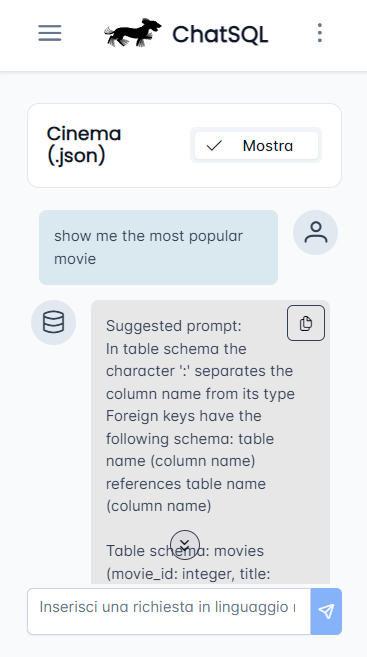
\includegraphics[width=0.50\textwidth]{assets/mobile.png}
  \caption{Versione mobile dell'applicazione}
\end{figure}
\par L'applicazione è stata progettata per essere fruibile anche da dispositivi mobili per garantire una buona esperienza d'uso con schermi touch screen di piccole dimensioni.  
\par Per migliorare la navigazione da dispositivi mobili, il menù principale, di default è nascosto e può essere aperto cliccando l'icona a tre linee 
\includegraphics[height=1.2em]{assets/dd_burger_menu.png} in alto a sinistra.
\par Le viste dell'applicazione occupano tutta la grandezza dello schermo, per dare più spazio possibile al contenuto principale.
\par Per ridurre l'ingombro dello schermo, i bottoni di login e delle impostazioni di sistema, sono accessibili mostrando un menù a tendina, cliccando sull'icona a tre puntini 
\includegraphics[height=1.2em]{assets/dd_kebab_menu.png} in alto a destra.



\end{document}